% !TEX program = pdflatex
\documentclass[11pt,a4paper]{article}

\usepackage[T1]{fontenc}
\usepackage{lmodern}
\usepackage{microtype}
\usepackage[margin=1in]{geometry}
\usepackage{indentfirst}
\usepackage{graphicx}
\usepackage{float}
\usepackage{caption}
\usepackage{subcaption}
\usepackage{booktabs}
\usepackage{array}
\usepackage{multirow}
\usepackage[section]{placeins}
\usepackage{tablefootnote}
\usepackage{enumitem}
\usepackage[table]{xcolor}
\usepackage{amsmath, amssymb}
\usepackage{amsthm}
\usepackage{algorithm}
\usepackage{algpseudocode}
\usepackage{tikz}
\usetikzlibrary{arrows.meta, calc, positioning, shapes.geometric}
\usepackage{pgfplots}
\pgfplotsset{compat=1.18}
\usepackage[most]{tcolorbox}
\usepackage[numbers]{natbib}
\usepackage[titles]{tocloft}
\usepackage{hyperref}

\setlist{itemsep=2pt, topsep=4pt}
\setcounter{tocdepth}{2}
\setlength{\cftbeforesecskip}{0pt}
\makeatletter
\setlength{\@fptop}{0pt}\setlength{\@fpsep}{20pt plus 4pt}\setlength{\@fpbot}{0pt plus 1fil}
\makeatother
\newcolumntype{P}[1]{>{\raggedright\arraybackslash}p{#1}}
\captionsetup{font=small}
\setlength{\abovecaptionskip}{6pt}
\renewcommand{\topfraction}{0.85}\renewcommand{\bottomfraction}{0.7}
\renewcommand{\textfraction}{0.1}\renewcommand{\floatpagefraction}{0.75}
\setcounter{topnumber}{3}\setcounter{bottomnumber}{2}\setcounter{totalnumber}{5}
\setlength{\floatsep}{18pt plus 4pt minus 2pt}
\setlength{\textfloatsep}{20pt plus 4pt minus 4pt}
\setlength{\intextsep}{18pt plus 4pt minus 2pt}

\definecolor{rblue}{HTML}{2E2E9C}
\definecolor{rbluedk}{HTML}{1C1C6B}
\definecolor{rbluemd}{HTML}{5A5AC4}
\definecolor{rbluelt}{HTML}{E7E7F7}
\definecolor{cbOrange}{HTML}{D97706}
\definecolor{cbOrangeLt}{HTML}{FDF0DC}
\definecolor{cbGreen}{HTML}{0B7A3B}
\definecolor{cbGreenLt}{HTML}{E4F2E9}
\definecolor{cbRed}{HTML}{B01B2E}
\definecolor{cbRedLt}{HTML}{FAE7E9}
\definecolor{neutralg}{gray}{0.46}
\definecolor{hlyellow}{HTML}{FFE9A8}
\definecolor{gridgray}{gray}{0.82}
\definecolor{closedc}{gray}{0.80}
\definecolor{gfree}{HTML}{F4EDEE}
\definecolor{gopen}{HTML}{DEBBC2}
\definecolor{gclose}{HTML}{BE7F89}
\definecolor{gwall}{HTML}{3F3F46}
\definecolor{gstart}{HTML}{0B7A3B}
\definecolor{ggoal}{HTML}{B01B2E}
\definecolor{blkInk}{HTML}{20242E}
\colorlet{algdijkstra}{rbluemd}
\colorlet{alggreedy}{cbOrange}
\colorlet{algastar}{cbGreen}
\definecolor{inkgray}{gray}{0.40}

\hypersetup{colorlinks=true, linkcolor=rbluedk, citecolor=rbluedk,
            urlcolor=rbluedk, pdftitle={The A* Search Algorithm},
            pdfauthor={Zarif Ishmam, Tonmoy Biswas, Proteek Rosul}}

\theoremstyle{plain}
\newtheorem{theorem}{Theorem}
\newtheorem{lemma}{Lemma}
\newtheorem{proposition}{Proposition}
\newtheorem{corollary}{Corollary}
\theoremstyle{definition}
\newtheorem{definition}{Definition}
\newtheorem{example}{Example}
\newtheorem{remark}{Remark}

\tcbset{rptbox/.style={enhanced, boxrule=0.6pt, arc=2pt,
        left=6pt, right=6pt, top=4pt, bottom=4pt,
        before skip=8pt, after skip=8pt}}
\tcolorboxenvironment{definition}{rptbox, colback=rbluelt!45, colframe=rblue!70}
\tcolorboxenvironment{theorem}{rptbox, colback=cbGreenLt!70, colframe=cbGreen!80}
\tcolorboxenvironment{lemma}{rptbox, colback=cbGreenLt!45, colframe=cbGreen!55}
\tcolorboxenvironment{proposition}{rptbox, colback=cbGreenLt!45, colframe=cbGreen!55}
\tcolorboxenvironment{corollary}{rptbox, colback=cbGreenLt!45, colframe=cbGreen!55}
\tcolorboxenvironment{example}{rptbox, colback=cbOrangeLt!60, colframe=cbOrange!70}

\newcommand{\cty}[1]{\textsf{#1}}

\algrenewcommand\algorithmicrequire{\textbf{Input:}}
\algrenewcommand\algorithmicensure{\textbf{Output:}}
\newcommand{\nil}{\textsc{nil}}

\makeatletter\newcommand{\inputrows}[1]{\@@input #1 }\makeatother

\makeatletter
\AtBeginDocument{%
  \expandafter\renewcommand\expandafter\subsection\expandafter
    {\expandafter\@fb@secFB\subsection}%
  \expandafter\renewcommand\expandafter\subsubsection\expandafter
    {\expandafter\@fb@secFB\subsubsection}}
\makeatother

\newcommand{\repourl}{https://github.com/ishmamzarif/a-star-report}

\tikzset{
  maplandfill/.style = {fill=gray!8},
  mapborder/.style   = {draw=gray!55, line width=0.5pt, line join=round},
  mapedge/.style     = {draw=gray!40, line width=0.35pt},
  mapdot/.style      = {circle, fill=white, draw=gray!60, line width=0.3pt,
                        minimum size=1.3mm, inner sep=0pt},
  mapstart/.style    = {circle, fill=algastar, draw=white, line width=0.5pt,
                        minimum size=2.2mm, inner sep=0pt},
  mapgoal/.style     = {circle, fill=cbRed, draw=white, line width=0.5pt,
                        minimum size=2.2mm, inner sep=0pt},
  maplabel/.style    = {font=\footnotesize, inner sep=2pt},
  maproute/.style    = {line width=1.3pt, line cap=round, line join=round},
  gridline/.style    = {draw=gray!35, line width=0.2pt},
  gridletter/.style  = {circle, text=white, font=\tiny\bfseries,
                        minimum size=2.6mm, inner sep=0pt},
  storyedge/.style   = {draw=rblue!55, line width=0.8pt},
  storyweight/.style = {fill=white, font=\footnotesize, inner sep=1.2pt,
                        text=rbluedk},
  storynode/.style   = {circle, draw=rblue, fill=white, line width=0.8pt,
                        minimum size=6mm, inner sep=0pt, font=\small\bfseries},
  storystart/.style  = {storynode, draw=algastar, fill=algastar!12},
  storygoal/.style   = {storynode, draw=cbRed, fill=cbRed!10},
  storyh/.style      = {font=\footnotesize, inner sep=0pt},
}

\providecolor{crimson}{HTML}{B01B2E}
\newcommand{\gpad}{0.075}
\newcommand{\gcell}[3]{%
  \fill[#1] ({#2+\gpad},{#3+\gpad}) rectangle ({#2+1-\gpad},{#3+1-\gpad});}
\tikzset{
  edgpath/.style   = {draw=cbGreen, line width=2.2pt},
  edgorange/.style = {draw=cbOrange, line width=2.2pt},
  wlab/.style      = {font=\scriptsize, fill=white, inner sep=1pt, text=rbluedk},
  visible on/.style = {},
  vball/.style  = {circle, fill=hlyellow, draw=cbOrange, line width=1pt,
                   minimum size=3.4mm, inner sep=0pt},
  move3d/.style = {-{Stealth[length=2.2mm]}, line width=1.7pt,
                   line cap=round, shorten >=0.6pt},
  isoweight/.style = {font=\scriptsize, text=rbluedk, fill=rbluelt!35,
                      inner sep=1.2pt, rounded corners=1pt},
}
\pgfplotsset{colormap={htiles}{color=(gfree) color=(gclose) color=(gstart) color=(ggoal)}}
\newcommand{\isodisc}[5]{%
  \colorlet{discrim}{#3}%
  \fill[black, opacity=0.10] ($(#1)+(0.04,-0.08)$) ellipse (0.34 and 0.22);
  \fill[discrim!25] ($(#1)+(-0.33,0)$) -- ++(0,0.13)
    arc[start angle=180, end angle=360, x radius=0.33, y radius=0.27]
    -- ++(0,-0.13) arc[start angle=0, end angle=-180, x radius=0.33, y radius=0.27];
  \draw[draw=#3, fill=#2, line width=0.85pt] ($(#1)+(0,0.13)$) ellipse (0.33 and 0.27);
  \node[font=\small\sffamily\bfseries, text=rbluedk, inner sep=0pt] at ($(#1)+(0,0.22)$) {#4};
  \node[font=\scriptsize, text=cbOrange!85!black, inner sep=0pt]
    at ($(#1)+(0,0.02)$) {$#5$};}

\providecolor{crimson}{HTML}{B01B2E}
\tikzset{
  bdcoast/.style  = {draw=gridgray, line width=0.7pt,
                     dash pattern=on 2.0pt off 1.6pt, rounded corners=0.8pt},
  bdland/.style   = {fill=black!3},
  bdedge/.style   = {draw=gridgray, line width=0.3pt,
                     dash pattern=on 1.1pt off 1.1pt},
  bdcity/.style   = {circle, fill=neutralg, draw=none,
                     minimum size=1.25mm, inner sep=0pt},
  bdlab/.style    = {font=\fontsize{4.0}{4.6}\selectfont, text=neutralg,
                     inner sep=1pt},
  bdlabhi/.style  = {bdlab, text=rbluedk,
                     font=\fontsize{4.4}{5}\selectfont\bfseries},
}
\newcommand{\bdbase}{%
    \draw[bdcoast, bdland]
      (88.32,26.52) -- (88.45,26.63) -- (88.62,26.44) -- (88.72,26.18) --
      (88.90,26.30) -- (89.05,26.36) -- (89.22,26.22) -- (89.38,26.42) --
      (89.58,26.18) -- (89.68,26.30) -- (89.82,26.02) -- (89.86,25.72) --
      (89.96,25.34) -- (90.18,25.20) -- (90.48,25.15) -- (90.72,25.23) --
      (91.02,25.17) -- (91.28,25.21) -- (91.58,25.12) -- (91.82,25.20) --
      (92.06,25.17) -- (92.30,25.04) -- (92.36,24.82) -- (92.16,24.54) --
      (92.06,24.24) -- (91.76,24.14) -- (91.60,23.98) -- (91.46,23.74) --
      (91.56,23.54) -- (91.40,23.34) -- (91.20,23.18) -- (91.36,23.04) --
      (91.58,22.96) -- (92.02,23.16) -- (92.26,23.24) -- (92.36,22.98) --
      (92.20,22.70) -- (92.46,22.34) -- (92.62,22.14) -- (92.58,21.92) --
      (92.50,21.58) -- (92.41,21.28) -- (92.36,21.02) -- (92.32,20.75) --
      (92.18,20.95) -- (92.06,21.20) -- (91.96,21.44) -- (91.88,21.70) --
      (91.80,21.96) -- (91.70,22.18) -- (91.52,22.42) -- (91.32,22.60) --
      (91.20,22.74) -- (91.08,22.28) -- (90.98,22.56) -- (90.86,22.20) --
      (90.74,22.00) -- (90.58,22.44) -- (90.46,22.12) -- (90.34,21.92) --
      (90.22,21.80) -- (90.04,21.96) -- (89.88,21.88) -- (89.68,21.84) --
      (89.48,21.76) -- (89.28,21.80) -- (89.10,21.92) -- (88.98,22.14) --
      (88.84,22.34) -- (88.72,22.60) -- (88.90,23.00) -- (88.74,23.26) --
      (88.58,23.50) -- (88.50,23.80) -- (88.86,24.02) -- (88.58,24.20) --
      (88.30,24.30) -- (88.04,24.56) -- (87.98,24.86) -- (88.14,25.16) --
      (88.40,25.22) -- (88.56,25.50) -- (88.30,25.76) -- (88.10,25.96) --
      (88.18,26.26) --
      cycle;

    \coordinate (panchagarh)      at (88.55,26.33);
    \coordinate (thakurgaon)      at (88.46,26.03);
    \coordinate (nilphamari)      at (88.86,25.93);
    \coordinate (lalmonirhat)     at (89.45,25.92);
    \coordinate (kurigram)        at (89.65,25.81);
    \coordinate (rangpur)         at (89.24,25.75);
    \coordinate (dinajpur)        at (88.64,25.63);
    \coordinate (gaibandha)       at (89.54,25.33);
    \coordinate (joypurhat)       at (89.03,25.09);
    \coordinate (sunamganj)       at (91.40,25.07);
    \coordinate (sherpur)         at (90.02,25.02);
    \coordinate (jamalpur)        at (89.94,24.92);
    \coordinate (sylhet)          at (91.87,24.90);
    \coordinate (netrokona)       at (90.73,24.88);
    \coordinate (bogura)          at (89.37,24.85);
    \coordinate (naogaon)         at (88.94,24.80);
    \coordinate (mymensingh)      at (90.40,24.75);
    \coordinate (chapainawabganj) at (88.28,24.60);
    \coordinate (moulvibazar)     at (91.78,24.48);
    \coordinate (sirajganj)       at (89.71,24.45);
    \coordinate (kishoreganj)     at (90.78,24.44);
    \coordinate (natore)          at (89.00,24.42);
    \coordinate (rajshahi)        at (88.60,24.37);
    \coordinate (habiganj)        at (91.42,24.37);
    \coordinate (tangail)         at (89.92,24.25);
    \coordinate (pabna)           at (89.24,24.00);
    \coordinate (gazipur)         at (90.42,23.99);
    \coordinate (brahmanbaria)    at (91.11,23.96);
    \coordinate (narsingdi)       at (90.72,23.92);
    \coordinate (kushtia)         at (89.12,23.90);
    \coordinate (manikganj)       at (90.00,23.86);
    \coordinate (dhaka)           at (90.41,23.81);
    \coordinate (meherpur)        at (88.63,23.77);
    \coordinate (rajbari)         at (89.64,23.76);
    \coordinate (chuadanga)       at (88.85,23.64);
    \coordinate (narayanganj)     at (90.50,23.62);
    \coordinate (faridpur)        at (89.84,23.60);
    \coordinate (munshiganj)      at (90.53,23.55);
    \coordinate (jhenaidah)       at (89.17,23.54);
    \coordinate (magura)          at (89.42,23.49);
    \coordinate (cumilla)         at (91.18,23.46);
    \coordinate (chandpur)        at (90.66,23.23);
    \coordinate (shariatpur)      at (90.35,23.20);
    \coordinate (jashore)         at (89.21,23.17);
    \coordinate (narail)          at (89.50,23.16);
    \coordinate (madaripur)       at (90.19,23.16);
    \coordinate (khagrachhari)    at (91.98,23.10);
    \coordinate (feni)            at (91.40,23.02);
    \coordinate (gopalganj)       at (89.83,23.01);
    \coordinate (lakshmipur)      at (90.83,22.94);
    \coordinate (noakhali)        at (91.10,22.87);
    \coordinate (khulna)          at (89.56,22.82);
    \coordinate (satkhira)        at (89.07,22.72);
    \coordinate (barishal)        at (90.37,22.70);
    \coordinate (bhola)           at (90.65,22.69);
    \coordinate (bagerhat)        at (89.79,22.65);
    \coordinate (rangamati)       at (92.17,22.65);
    \coordinate (jhalokati)       at (90.20,22.64);
    \coordinate (pirojpur)        at (89.98,22.58);
    \coordinate (patuakhali)      at (90.33,22.36);
    \coordinate (chattogram)      at (91.78,22.36);
    \coordinate (bandarban)       at (92.22,22.19);
    \coordinate (barguna)         at (90.13,22.15);
    \coordinate (coxsbazar)       at (92.01,21.44);

    \foreach \a/\b in {%
      panchagarh/thakurgaon, panchagarh/nilphamari, thakurgaon/dinajpur,
      nilphamari/dinajpur, nilphamari/rangpur, nilphamari/lalmonirhat,
      lalmonirhat/rangpur, lalmonirhat/kurigram, dinajpur/rangpur,
      dinajpur/joypurhat, dinajpur/naogaon, rangpur/kurigram,
      rangpur/gaibandha, kurigram/gaibandha, gaibandha/bogura,
      gaibandha/joypurhat, gaibandha/jamalpur, joypurhat/naogaon,
      joypurhat/bogura, naogaon/bogura, naogaon/natore,
      naogaon/chapainawabganj, naogaon/rajshahi, chapainawabganj/rajshahi,
      rajshahi/natore, natore/bogura, natore/sirajganj,
      natore/pabna, natore/kushtia, bogura/sirajganj,
      sirajganj/pabna, sirajganj/tangail, sirajganj/jamalpur,
      pabna/kushtia, pabna/rajbari, kushtia/chuadanga,
      kushtia/jhenaidah, kushtia/meherpur, kushtia/rajbari,
      meherpur/chuadanga, chuadanga/jhenaidah, chuadanga/jashore,
      jhenaidah/magura, jhenaidah/jashore, magura/narail,
      magura/faridpur, magura/rajbari, narail/jashore,
      narail/khulna, narail/gopalganj, jashore/satkhira,
      jashore/khulna, satkhira/khulna, khulna/bagerhat,
      bagerhat/pirojpur, bagerhat/gopalganj, gopalganj/faridpur,
      gopalganj/madaripur, gopalganj/pirojpur, gopalganj/barishal,
      rajbari/faridpur, rajbari/manikganj, faridpur/madaripur,
      faridpur/manikganj, madaripur/shariatpur, madaripur/barishal,
      shariatpur/chandpur, shariatpur/munshiganj, shariatpur/barishal,
      pirojpur/jhalokati, pirojpur/barguna, pirojpur/barishal,
      jhalokati/barishal, jhalokati/barguna, jhalokati/patuakhali,
      barguna/patuakhali, patuakhali/barishal, patuakhali/bhola,
      barishal/bhola, bhola/lakshmipur, bhola/noakhali,
      lakshmipur/noakhali, lakshmipur/chandpur, lakshmipur/cumilla,
      noakhali/cumilla, noakhali/feni, noakhali/chattogram,
      feni/cumilla, feni/chattogram, feni/khagrachhari,
      chandpur/cumilla, chandpur/munshiganj, cumilla/brahmanbaria,
      cumilla/munshiganj, brahmanbaria/narsingdi, brahmanbaria/kishoreganj,
      brahmanbaria/habiganj, brahmanbaria/narayanganj, narsingdi/kishoreganj,
      narsingdi/gazipur, narsingdi/narayanganj, narsingdi/dhaka,
      munshiganj/narayanganj, munshiganj/dhaka, munshiganj/manikganj,
      narayanganj/dhaka, dhaka/gazipur, dhaka/manikganj,
      gazipur/tangail, gazipur/mymensingh, gazipur/kishoreganj,
      manikganj/tangail, tangail/jamalpur, tangail/mymensingh,
      jamalpur/sherpur, jamalpur/mymensingh, sherpur/mymensingh,
      mymensingh/netrokona, mymensingh/kishoreganj, netrokona/kishoreganj,
      netrokona/sunamganj, kishoreganj/habiganj, habiganj/sunamganj,
      habiganj/moulvibazar, sunamganj/sylhet, sylhet/moulvibazar,
      khagrachhari/rangamati, khagrachhari/chattogram, rangamati/chattogram,
      rangamati/bandarban, bandarban/chattogram, bandarban/coxsbazar,
      chattogram/coxsbazar}
      {\draw[bdedge] (\a)--(\b);}

    \foreach \n in {bagerhat, bandarban, barguna, barishal, bhola, bogura,
      brahmanbaria, chandpur, chapainawabganj, chattogram, chuadanga, coxsbazar,
      cumilla, dhaka, dinajpur, faridpur, feni, gaibandha,
      gazipur, gopalganj, habiganj, jamalpur, jashore, jhalokati,
      jhenaidah, joypurhat, khagrachhari, khulna, kishoreganj, kurigram,
      kushtia, lakshmipur, lalmonirhat, madaripur, magura, manikganj,
      meherpur, moulvibazar, munshiganj, mymensingh, naogaon, narail,
      narayanganj, narsingdi, natore, netrokona, nilphamari, noakhali,
      pabna, panchagarh, patuakhali, pirojpur, rajbari, rajshahi,
      rangamati, rangpur, satkhira, shariatpur, sherpur, sirajganj,
      sunamganj, sylhet, tangail, thakurgaon}
      {\node[bdcity] at (\n) {};}
}

\tikzset{
  cam/.code n args = {4}{%
    \pgfmathsetmacro\camxx{(#3)*cos(#1)}%
    \pgfmathsetmacro\camxy{-(#3)*sin(#1)*sin(#2)}%
    \pgfmathsetmacro\camyx{(#4)*sin(#1)}%
    \pgfmathsetmacro\camyy{(#4)*cos(#1)*sin(#2)}%
    \pgfmathsetmacro\camzy{(#4)*cos(#2)}%
    \edef\camkeys{\noexpand\pgfkeysalso{%
      x={(\camxx cm,\camxy cm)}, y={(\camyx cm,\camyy cm)},
      z={(0cm,\camzy cm)}}}%
    \camkeys},
  necam/.style = {cam={20}{40}{2.45}{2.7}},
}

\pgfplotsset{
  colormap={hblue}{color=(rbluedk) color=(rbluemd) color=(rbluelt)},
  colormap={horange}{color=(cbOrange!70!black) color=(cbOrange) color=(cbOrangeLt)},
  colormap={hgreen}{color=(cbGreen!70!black) color=(cbGreen) color=(cbGreenLt)},
  land3d/.style   = {axis lines=none, clip=false},
  land view/.code n args = {3}{%
    \pgfmathsetmacro\lvxx{#3*cos(#1)}%
    \pgfmathsetmacro\lvxy{-#3*sin(#1)*sin(#2)}%
    \pgfmathsetmacro\lvyx{#3*sin(#1)}%
    \pgfmathsetmacro\lvyy{#3*cos(#1)*sin(#2)}%
    \pgfmathsetmacro\lvzy{#3*cos(#2)}%
    \edef\lvkeys{\noexpand\pgfkeysalso{%
      x={(\lvxx cm,\lvxy cm)}, y={(\lvyx cm,\lvyy cm)}, z={(0cm,\lvzy cm)}}}%
    \lvkeys},
  tilesurf/.style = {surf, shader=faceted, faceted color=white,
                     line width=0.4pt, z buffer=sort, point meta=z},
}

\tikzset{
  sball/.style    = {circle, fill=gstart, draw=white, line width=0.7pt,
                     minimum size=3.2mm, inner sep=0pt},
  gball/.style    = {sball, fill=ggoal},
  cball/.style    = {sball, fill=hlyellow, draw=cbOrange, line width=1pt},
  oball/.style    = {sball, fill=white, draw=rblue, line width=0.9pt,
                     minimum size=2.6mm},
  tag/.style      = {font=\scriptsize, inner sep=1.5pt},
  tagbox/.style   = {tag, fill=white, fill opacity=0.88, text opacity=1,
                     rounded corners=1pt},
  maplab/.style   = {font=\fontsize{5.6}{6.4}\selectfont, text=neutralg,
                     inner sep=1pt},
  liftedge/.style = {draw=rblue!80, line width=0.75pt},
  liftnode/.style = {circle, fill=rbluemd, draw=white, line width=0.3pt,
                     minimum size=1.5mm, inner sep=0pt},
  dropline/.style = {draw=rblue!28, line width=0.3pt},
  pin/.style      = {line width=0.55pt, line cap=butt},
  pinhead/.style  = {circle, draw=white, line width=0.25pt,
                     minimum size=1.3mm, inner sep=0pt},
  water/.style    = {fill=rbluelt, fill opacity=0.62},
  waterrim/.style = {draw=rbluemd, line width=0.5pt},
  latedge/.style  = {draw=gridgray, line width=0.55pt},
  latnode/.style  = {circle, fill=white, draw=neutralg, line width=0.45pt,
                     minimum size=1.7mm, inner sep=0pt},
}

\newcommand{\bddata}{%
  bagerhat/172.0/327.7, bandarban/273.7/303.4, barguna/199.2/353.5,
  barishal/130.1/288.3, bhola/139.4/275.3, bogura/165.4/252.3,
  brahmanbaria/73.7/129.8, chandpur/69.4/222.7, chapainawabganj/263.3/364.0,
  chattogram/224.7/282.6, chuadanga/175.4/336.7, coxsbazar/329.7/385.0,
  cumilla/98.4/174.7, dhaka/0.0/191.2, dinajpur/280.6/334.8,
  faridpur/75.3/251.5, feni/152.3/214.4, gaibandha/213.8/239.4,
  gazipur/20.0/178.3, gopalganj/131.8/295.2, habiganj/129.1/74.4,
  jamalpur/153.0/194.7, jashore/185.1/331.6, jhalokati/148.7/303.4,
  jhenaidah/143.9/312.8, joypurhat/208.9/287.0, khagrachhari/212.3/200.5,
  khulna/193.7/329.6, kishoreganj/82.0/121.4, kurigram/268.3/244.9,
  kushtia/135.5/299.8, lakshmipur/106.0/242.2, lalmonirhat/291.8/268.2,
  madaripur/91.4/258.0, magura/117.8/293.8, manikganj/42.1/221.9,
  meherpur/187.4/351.5, moulvibazar/167.5/47.6, munshiganj/31.4/202.5,
  mymensingh/104.6/149.3, naogaon/209.2/295.8, narail/155.4/308.8,
  narayanganj/23.0/198.9, narsingdi/33.8/159.5, natore/181.2/294.9,
  netrokona/131.2/115.0, nilphamari/312.3/323.3, noakhali/134.7/238.9,
  pabna/129.0/284.4, panchagarh/363.1/368.9, patuakhali/168.1/323.1,
  pirojpur/172.2/321.8, rajbari/80.3/259.1, rajshahi/222.1/335.7,
  rangamati/266.0/252.0, rangpur/269.4/280.7, satkhira/237.1/374.0,
  shariatpur/74.4/244.0, sherpur/153.3/187.0, sirajganj/109.2/223.9,
  sunamganj/201.9/51.0, sylhet/215.1/0.0, tangail/78.4/210.0,
  thakurgaon/328.5/364.7}
\newcommand{\bddjorder}{dhaka, gazipur, narayanganj, munshiganj, narsingdi, manikganj, chandpur, brahmanbaria, shariatpur, faridpur, tangail, rajbari, kishoreganj, madaripur, cumilla, mymensingh, lakshmipur, sirajganj, magura, pabna, habiganj, barishal, netrokona, gopalganj, noakhali, kushtia, bhola, jhenaidah, jhalokati, feni, jamalpur, sherpur, narail, bogura, moulvibazar, patuakhali, bagerhat, pirojpur, chuadanga, natore, jashore, meherpur, khulna, barguna, sunamganj, joypurhat, naogaon, khagrachhari, gaibandha, sylhet}
\newcommand{\bddjroute}{(dhaka) -- (narsingdi) -- (brahmanbaria) -- (habiganj) -- (moulvibazar) -- (sylhet)}
\newcommand{\bdgrorder}{dhaka, narsingdi, kishoreganj, habiganj, moulvibazar, sylhet}
\newcommand{\bdgrroute}{(dhaka) -- (narsingdi) -- (kishoreganj) -- (habiganj) -- (moulvibazar) -- (sylhet)}
\newcommand{\bdasorder}{dhaka, narsingdi, gazipur, kishoreganj, brahmanbaria, habiganj, moulvibazar, sylhet}
\newcommand{\bdasroute}{(dhaka) -- (narsingdi) -- (brahmanbaria) -- (habiganj) -- (moulvibazar) -- (sylhet)}

\foreach \n/\vg/\vh in \bddata {%
  \expandafter\xdef\csname bdg@\n\endcsname{\vg}%
  \expandafter\xdef\csname bdh@\n\endcsname{\vh}}
\newcommand{\bdG}[1]{\csname bdg@#1\endcsname}
\newcommand{\bdH}[1]{\csname bdh@#1\endcsname}

\newcommand{\kz}{0.01}
\newcommand{\bdlift}[2]{($(#1)+(0,0,{(#2)*\kz})$)}
\newcommand{\bdup}[1]{\bdlift{#1}{\bdG{#1}}}

\newcommand{\bdcoastpath}{%
  (88.32,26.52) -- (88.45,26.63) -- (88.62,26.44) -- (88.72,26.18) --
  (88.90,26.30) -- (89.05,26.36) -- (89.22,26.22) -- (89.38,26.42) --
  (89.58,26.18) -- (89.68,26.30) -- (89.82,26.02) -- (89.86,25.72) --
  (89.96,25.34) -- (90.18,25.20) -- (90.48,25.15) -- (90.72,25.23) --
  (91.02,25.17) -- (91.28,25.21) -- (91.58,25.12) -- (91.82,25.20) --
  (92.06,25.17) -- (92.30,25.04) -- (92.36,24.82) -- (92.16,24.54) --
  (92.06,24.24) -- (91.76,24.14) -- (91.60,23.98) -- (91.46,23.74) --
  (91.56,23.54) -- (91.40,23.34) -- (91.20,23.18) -- (91.36,23.04) --
  (91.58,22.96) -- (92.02,23.16) -- (92.26,23.24) -- (92.36,22.98) --
  (92.20,22.70) -- (92.46,22.34) -- (92.62,22.14) -- (92.58,21.92) --
  (92.50,21.58) -- (92.41,21.28) -- (92.36,21.02) -- (92.32,20.75) --
  (92.18,20.95) -- (92.06,21.20) -- (91.96,21.44) -- (91.88,21.70) --
  (91.80,21.96) -- (91.70,22.18) -- (91.52,22.42) -- (91.32,22.60) --
  (91.20,22.74) -- (91.08,22.28) -- (90.98,22.56) -- (90.86,22.20) --
  (90.74,22.00) -- (90.58,22.44) -- (90.46,22.12) -- (90.34,21.92) --
  (90.22,21.80) -- (90.04,21.96) -- (89.88,21.88) -- (89.68,21.84) --
  (89.48,21.76) -- (89.28,21.80) -- (89.10,21.92) -- (88.98,22.14) --
  (88.84,22.34) -- (88.72,22.60) -- (88.90,23.00) -- (88.74,23.26) --
  (88.58,23.50) -- (88.50,23.80) -- (88.86,24.02) -- (88.58,24.20) --
  (88.30,24.30) -- (88.04,24.56) -- (87.98,24.86) -- (88.14,25.16) --
  (88.40,25.22) -- (88.56,25.50) -- (88.30,25.76) -- (88.10,25.96) --
  (88.18,26.26) -- cycle}

\newcommand{\bdfloor}{%
  \begin{scope}[shift={(-87.98,-20.75)}]\bdbase\end{scope}}
\newcommand{\nefloor}{%
  \begin{scope}[shift={(-87.98,-20.75)}]
    \fill[black!2] (90.2,23.5) -- (92.2,23.5) -- (92.2,25.25)
                   -- (90.2,25.25) -- cycle;
    \begin{scope}
      \clip (90.2,23.5) -- (92.2,23.5) -- (92.2,25.25) -- (90.2,25.25) -- cycle;
      \bdbase
    \end{scope}
    \draw[gridgray, line width=0.4pt] (90.2,23.5) -- (92.2,23.5)
      -- (92.2,25.25) -- (90.2,25.25) -- cycle;
  \end{scope}}

\newcommand{\colw}{0.032}
\newcommand{\prism}[4]{%
  \fill[#4, draw=white, line width=0.2pt]
    ($(#1)+(-\colw,-\colw,{(#2)*\kz})$) -- ($(#1)+(\colw,-\colw,{(#2)*\kz})$)
    -- ($(#1)+(\colw,-\colw,{(#3)*\kz})$) -- ($(#1)+(-\colw,-\colw,{(#3)*\kz})$)
    -- cycle;
  \fill[#4!70!black, draw=white, line width=0.2pt]
    ($(#1)+(\colw,-\colw,{(#2)*\kz})$) -- ($(#1)+(\colw,\colw,{(#2)*\kz})$)
    -- ($(#1)+(\colw,\colw,{(#3)*\kz})$) -- ($(#1)+(\colw,-\colw,{(#3)*\kz})$)
    -- cycle;
  \fill[#4!45!white, draw=white, line width=0.2pt]
    ($(#1)+(-\colw,-\colw,{(#3)*\kz})$) -- ($(#1)+(\colw,-\colw,{(#3)*\kz})$)
    -- ($(#1)+(\colw,\colw,{(#3)*\kz})$) -- ($(#1)+(-\colw,\colw,{(#3)*\kz})$)
    -- cycle;}

\newcommand{\ptile}[3]{%
  \fill[#1] ({#2+\gpad},{#3+\gpad},0) -- ({#2+1-\gpad},{#3+\gpad},0)
    -- ({#2+1-\gpad},{#3+1-\gpad},0) -- ({#2+\gpad},{#3+1-\gpad},0) -- cycle;}
\newcommand{\wallh}{0.55}
\newcommand{\pblock}[2]{%
  \fill[gwall!78!white]
    ({#1+\gpad},{#2+\gpad},0) -- ({#1+1-\gpad},{#2+\gpad},0)
    -- ({#1+1-\gpad},{#2+\gpad},\wallh) -- ({#1+\gpad},{#2+\gpad},\wallh) -- cycle;
  \fill[gwall]
    ({#1+\gpad},{#2+\gpad},0) -- ({#1+\gpad},{#2+1-\gpad},0)
    -- ({#1+\gpad},{#2+1-\gpad},\wallh) -- ({#1+\gpad},{#2+\gpad},\wallh) -- cycle;
  \fill[gwall!45!white]
    ({#1+\gpad},{#2+\gpad},\wallh) -- ({#1+1-\gpad},{#2+\gpad},\wallh)
    -- ({#1+1-\gpad},{#2+1-\gpad},\wallh) -- ({#1+\gpad},{#2+1-\gpad},\wallh) -- cycle;}

\newcommand{\lifttree}[2]{{%
  \foreach \a/\b in {#2}{\draw[dropline] (\b) -- \bdup{\b};}%
  \foreach \a/\b in {#2}{\draw[liftedge] \bdup{\a} -- \bdup{\b};}%
  \foreach \a/\b in {#2}{\node[liftnode] at \bdup{\b} {};}}}

\newcommand{\wlevel}{215.1}
\newcommand{\pincap}{365}
\newcommand{\waterpanel}[2]{%
  \begin{tikzpicture}[cam={16}{24}{0.84}{0.92}]
    \def\kz{0.0062}
    \begin{scope}[bdedge/.style={draw=none}]\bdfloor\end{scope}
    \foreach \n/\vg/\vh in \bddata {%
      \pgfmathsetmacro\pz{\vg+#1*\vh}%
      \pgfmathtruncatemacro\sub{\pz <= \wlevel+0.05}%
      \ifnum\sub=1
        \draw[pin, draw=#2] (\n) -- \bdlift{\n}{\pz};
        \node[pinhead, fill=#2] at \bdlift{\n}{\pz} {};
      \else
        \draw[pin, draw=neutralg!30] (\n) -- \bdlift{\n}{\wlevel};
      \fi}
    \begin{scope}[shift={(-87.98,-20.75,{\wlevel*\kz})}]
      \fill[water] \bdcoastpath;
      \draw[waterrim] \bdcoastpath;
    \end{scope}
    \foreach \n/\vg/\vh in \bddata {%
      \path \bdlift{\n}{\pincap};
      \pgfmathsetmacro\pz{\vg+#1*\vh}%
      \pgfmathtruncatemacro\sub{\pz <= \wlevel+0.05}%
      \ifnum\sub=0
        \pgfmathsetmacro\pt{min(\pz,\pincap)}%
        \draw[pin, draw=neutralg!80] \bdlift{\n}{\wlevel} -- \bdlift{\n}{\pt};
        \pgfmathtruncatemacro\cut{\pz > \pincap}%
        \ifnum\cut=0
          \node[pinhead, fill=neutralg!70, minimum size=1.0mm]
            at \bdlift{\n}{\pz} {};
        \fi
      \fi}
    \node[gball, minimum size=2.2mm] at \bdlift{sylhet}{\wlevel} {};
    \node[sball, minimum size=2.2mm] at (dhaka) {};
  \end{tikzpicture}}

\newcommand{\djorder}{%
  1/4, 2/4, 0/4, 1/5, 1/3, 3/4, 2/5, 2/3, 0/5, 0/3, 1/6, 1/2, 4/4, 3/5,
  3/3, 2/6, 2/2, 0/6, 0/2, 1/7, 1/1, 5/4, 4/5, 3/6, 3/2, 2/7, 2/1, 0/7,
  0/1, 1/8, 1/0, 6/4, 5/5, 4/6, 3/7, 4/2, 3/1, 2/8, 2/0, 0/8, 0/0, 1/9,
  7/4, 6/5, 5/6, 3/8, 5/2, 4/1, 3/0, 2/9, 0/9, 8/4, 7/5, 6/6, 4/8, 3/9,
  6/2, 5/1, 4/0, 9/4, 8/5, 7/6, 5/8, 4/9, 7/2, 6/1, 5/0, 10/4, 9/5, 8/6,
  6/8, 5/9, 8/2, 7/1, 6/0, 11/4, 10/5, 9/6, 7/8, 6/9, 9/2, 8/1, 7/0, 11/5,
  10/6, 8/8, 7/9, 10/2, 9/1, 8/0, 11/6, 9/8, 8/9, 11/2, 10/1, 9/0, 10/8, 9/9,
  12/2, 11/1, 10/0, 11/8, 10/9, 13/2, 12/1, 11/0, 12/8, 11/9, 14/2, 13/3, 13/1, 12/0,
  13/8, 12/9, 15/2, 14/3, 14/1, 13/4, 13/0, 14/8, 13/9, 13/7, 15/3, 15/1, 14/4, 14/0,
  13/5, 15/8, 14/9, 14/7, 13/6, 15/4, 15/0, 14/5, 15/9, 15/7, 14/6}
\newcommand{\djroute}{(1.5,4.5) -- (2.5,4.5) -- (3.5,4.5) -- (3.5,5.5) -- (3.5,6.5) -- (3.5,7.5) -- (3.5,8.5) -- (4.5,8.5) -- (5.5,8.5) -- (6.5,8.5) -- (7.5,8.5) -- (8.5,8.5) -- (9.5,8.5) -- (10.5,8.5) -- (11.5,8.5) -- (12.5,8.5) -- (13.5,8.5) -- (14.5,8.5) -- (14.5,7.5) -- (14.5,6.5)}
\newcommand{\grorder}{%
  1/4, 2/4, 3/4, 4/4, 5/4, 6/4, 7/4, 8/4, 9/4, 10/4, 11/4, 11/5, 11/6, 10/6,
  10/5, 9/6, 9/5, 8/6, 8/5, 7/6, 7/5, 6/6, 6/5, 5/6, 5/5, 4/6, 4/5, 3/6,
  3/5, 2/6, 3/7, 2/5, 1/6, 2/7, 3/8, 4/8, 5/8, 6/8, 7/8, 8/8, 9/8, 10/8,
  11/8, 12/8, 13/8, 14/8, 14/7, 14/6}
\newcommand{\grroute}{(1.5,4.5) -- (2.5,4.5) -- (3.5,4.5) -- (4.5,4.5) -- (5.5,4.5) -- (6.5,4.5) -- (7.5,4.5) -- (8.5,4.5) -- (9.5,4.5) -- (10.5,4.5) -- (11.5,4.5) -- (11.5,5.5) -- (11.5,6.5) -- (10.5,6.5) -- (9.5,6.5) -- (8.5,6.5) -- (7.5,6.5) -- (6.5,6.5) -- (5.5,6.5) -- (4.5,6.5) -- (3.5,6.5) -- (3.5,7.5) -- (3.5,8.5) -- (4.5,8.5) -- (5.5,8.5) -- (6.5,8.5) -- (7.5,8.5) -- (8.5,8.5) -- (9.5,8.5) -- (10.5,8.5) -- (11.5,8.5) -- (12.5,8.5) -- (13.5,8.5) -- (14.5,8.5) -- (14.5,7.5) -- (14.5,6.5)}
\newcommand{\asorder}{%
  1/4, 2/4, 1/5, 3/4, 2/5, 1/6, 4/4, 3/5, 2/6, 5/4, 4/5, 3/6, 6/4, 5/5,
  4/6, 7/4, 6/5, 5/6, 8/4, 7/5, 6/6, 9/4, 8/5, 7/6, 10/4, 9/5, 8/6, 11/4,
  10/5, 9/6, 11/5, 10/6, 11/6, 0/4, 1/3, 2/3, 0/5, 3/3, 0/6, 1/7, 2/7, 3/7,
  0/3, 1/2, 2/2, 3/2, 0/7, 1/8, 2/8, 3/8, 4/2, 4/8, 5/2, 5/8, 6/2, 6/8,
  7/2, 7/8, 8/2, 8/8, 9/2, 9/8, 10/2, 10/8, 11/2, 11/8, 12/2, 12/8, 13/2, 13/8,
  14/2, 13/3, 14/8, 13/7, 14/3, 13/4, 14/7, 13/6, 14/4, 13/5, 14/6}
\newcommand{\asroute}{(1.5,4.5) -- (2.5,4.5) -- (3.5,4.5) -- (3.5,5.5) -- (3.5,6.5) -- (3.5,7.5) -- (3.5,8.5) -- (4.5,8.5) -- (5.5,8.5) -- (6.5,8.5) -- (7.5,8.5) -- (8.5,8.5) -- (9.5,8.5) -- (10.5,8.5) -- (11.5,8.5) -- (12.5,8.5) -- (13.5,8.5) -- (14.5,8.5) -- (14.5,7.5) -- (14.5,6.5)}

\newcommand{\greedyroute}{\grroute}
\newcommand{\astarroute}{\asroute}
\newcommand{\dijkstraroute}{\djroute}

\newcommand{\gfloorthree}{%
  \foreach \c in {0,...,15}{\foreach \r in {0,...,9}{\ptile{gfree}{\c}{\r}}}}
\newcommand{\gendsthree}{%
  \ptile{gstart}{1}{4}\ptile{ggoal}{14}{6}%
  \node[text=white, font=\scriptsize] at (1.5,4.5,0) {$s$};%
  \node[text=white, font=\scriptsize] at (14.5,6.5,0) {$t$};}
\newcommand{\gwallsthree}{%
  \foreach \c in {12,...,4}{\pblock{\c}{7}}%
  \foreach \r in {6,5,4}{\pblock{12}{\r}}%
  \foreach \c in {12,...,4}{\pblock{\c}{3}}}
\newcommand{\gexpand}[2]{{\foreach \c/\r in {#2}{\ptile{gclose}{\c}{\r}}}}

\tikzset{declare function={
  Efold(\x,\y) = 1.3 + 0.12*(\x*\x+\y*\y)
                 - 1.1*exp(-((\x+1.8)^2+\y*\y)/0.9)
                 - 1.6*exp(-((\x-1.8)^2+\y*\y)/0.8)
                 + 1.3*exp(-(\x*\x+(\y-0.2)^2)/0.7);}}

\foreach \c/\r [count=\n] in \djorder {\expandafter\xdef\csname dj-\c-\r\endcsname{\n}}
\foreach \c/\r [count=\n] in \asorder {\expandafter\xdef\csname as-\c-\r\endcsname{\n}}
\foreach \c in {4,...,12}{%
  \expandafter\xdef\csname wl-\c-3\endcsname{1}%
  \expandafter\xdef\csname wl-\c-7\endcsname{1}}
\foreach \r in {4,5,6}{\expandafter\xdef\csname wl-12-\r\endcsname{1}}

\newcommand{\pbox}[4]{%
  \fill[#4!85!black]
    ({#1+\gpad},{#2+\gpad},0) -- ({#1+1-\gpad},{#2+\gpad},0)
    -- ({#1+1-\gpad},{#2+\gpad},#3) -- ({#1+\gpad},{#2+\gpad},#3) -- cycle;
  \fill[#4!68!black]
    ({#1+\gpad},{#2+\gpad},0) -- ({#1+\gpad},{#2+1-\gpad},0)
    -- ({#1+\gpad},{#2+1-\gpad},#3) -- ({#1+\gpad},{#2+\gpad},#3) -- cycle;
  \fill[#4]
    ({#1+\gpad},{#2+\gpad},#3) -- ({#1+1-\gpad},{#2+\gpad},#3)
    -- ({#1+1-\gpad},{#2+1-\gpad},#3) -- ({#1+\gpad},{#2+1-\gpad},#3) -- cycle;}

\newcommand{\tstep}{0.052}
\newcommand{\timeview}[1]{%
  \begin{tikzpicture}[cam={-24}{40}{0.295}{0.295}, line join=round]
    \foreach \c in {0,...,15}{\foreach \r in {0,...,9}{\ptile{gfree}{\c}{\r}}}
    \foreach \r in {9,...,0}{\foreach \c in {15,...,0}{%
      \ifcsname #1-\c-\r\endcsname
        \edef\kk{\csname #1-\c-\r\endcsname}%
        \pgfmathsetmacro\zz{\kk*\tstep}%
        \pgfmathtruncatemacro\pc{15+85*\kk/137}%
        \def\colr{gclose!70!black!\pc!gopen}%
        \ifnum\c=1 \ifnum\r=4 \def\colr{gstart}\fi\fi
        \ifnum\c=14 \ifnum\r=6 \def\colr{ggoal}\fi\fi
        \pbox{\c}{\r}{\zz}{\colr}%
      \else
        \ifcsname wl-\c-\r\endcsname \pblock{\c}{\r}\fi
      \fi}}
  \end{tikzpicture}}

\foreach \c/\r [count=\n] in \grorder {\expandafter\xdef\csname gr-\c-\r\endcsname{\n}}

\newcommand{\gridpanel}[3]{%
  \begin{tikzpicture}[cam={-24}{54}{0.235}{0.235}, line cap=round,
                      line join=round]
    \foreach \c in {0,...,15}{\foreach \r in {0,...,9}{%
      \ifcsname #1-\c-\r\endcsname \ptile{gclose}{\c}{\r}%
      \else \ptile{gfree}{\c}{\r}\fi}}
    \ptile{gstart}{1}{4}\ptile{ggoal}{14}{6}
    \draw[#3, line width=1.4pt] #2;
    \gwallsthree
  \end{tikzpicture}}
\def\kA{0.45}\def\gAx{7}\def\gAy{3}
\newcommand{\liftA}[2]{(#1,#2,{\kA*veclen((#1)-\gAx,(#2)-\gAy)})}
\newcommand{\floorA}{%
  \pgfplotsinvokeforeach{0,...,12}{%
    \draw[gridgray, line width=0.35pt] (##1,0,0) -- (##1,12,0);
    \draw[gridgray, line width=0.35pt] (0,##1,0) -- (12,##1,0);}}

\def\kB{0.45}
\newcommand{\liftB}[2]{(#1,#2,{\kB*veclen(#1,#2)})}

\def\kC{0.3}
\def\cSx{5.5}\def\cSy{6.5}\def\cGx{10.5}\def\cGy{6.5}
\def\cCost{5}\def\cSlack{0.9}
\newcommand{\legendC}{%
  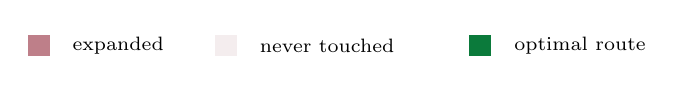
\begin{tikzpicture}[x=0.34cm,y=0.34cm, baseline=0pt]
    \renewcommand{\gpad}{0.09}%
    \gcell{gclose}{0}{0}
      \node[anchor=west, font=\scriptsize] at (1.4,0.5) {expanded};
    \gcell{gfree}{7}{0}
      \node[anchor=west, font=\scriptsize] at (8.4,0.5) {never touched};
    \gcell{cbGreen}{16.5}{0}
      \node[anchor=west, font=\scriptsize] at (17.9,0.5) {optimal route};
  \end{tikzpicture}}

\def\kE{0.8}\def\pEx{2}\def\pEy{1}
\colorlet{gmgrass}{cbGreen!24!white}
\colorlet{gmmud}{cbOrange!40!white}
\colorlet{gmwater}{rbluemd!45!cyan!38!white}
\colorlet{gmearth}{cbOrange!40!gwall}
\colorlet{gmwood}{cbOrange!60!gwall}
\foreach \c in {5,6}{\foreach \r in {0,...,6}{%
  \expandafter\xdef\csname gmw-\c-\r\endcsname{1}}}
\foreach \c/\r in {7/3, 8/3, 7/4, 8/4}{%
  \expandafter\xdef\csname gmm-\c-\r\endcsname{1}}

\newcommand{\gmfloor}{-0.42}
\newcommand{\gmband}{0.07}
\newcommand{\gmslab}[4]{%
  \fill[gmearth!90!black]
    (#1,#2,\gmfloor) -- ({#1+1},#2,\gmfloor) -- ({#1+1},#2,{#3-\gmband})
    -- (#1,#2,{#3-\gmband}) -- cycle;
  \fill[gmearth!68!black]
    (#1,#2,\gmfloor) -- (#1,{#2+1},\gmfloor) -- (#1,{#2+1},{#3-\gmband})
    -- (#1,#2,{#3-\gmband}) -- cycle;
  \fill[#4!80!black]
    (#1,#2,{#3-\gmband}) -- ({#1+1},#2,{#3-\gmband}) -- ({#1+1},#2,#3)
    -- (#1,#2,#3) -- cycle;
  \fill[#4!62!black]
    (#1,#2,{#3-\gmband}) -- (#1,{#2+1},{#3-\gmband}) -- (#1,{#2+1},#3)
    -- (#1,#2,#3) -- cycle;
  \fill[#4, draw=white, line width=0.3pt]
    (#1,#2,#3) -- ({#1+1},#2,#3) -- ({#1+1},{#2+1},#3) -- (#1,{#2+1},#3)
    -- cycle;}
\newcommand{\gmrock}[3]{%
  \fill[gwall!78!white]
    ({#1+.1},{#2+.1},0) -- ({#1+.9},{#2+.1},0) -- ({#1+.9},{#2+.1},#3)
    -- ({#1+.1},{#2+.1},#3) -- cycle;
  \fill[gwall]
    ({#1+.1},{#2+.1},0) -- ({#1+.1},{#2+.9},0) -- ({#1+.1},{#2+.9},#3)
    -- ({#1+.1},{#2+.1},#3) -- cycle;
  \fill[gwall!45!white]
    ({#1+.1},{#2+.1},#3) -- ({#1+.9},{#2+.1},#3) -- ({#1+.9},{#2+.9},#3)
    -- ({#1+.1},{#2+.9},#3) -- cycle;}
\newcommand{\gmtree}[2]{%
  \fill[black, opacity=0.16] ({#1+0.5},{#2+0.5},0) ellipse (0.15cm and 0.065cm);
  \fill[gmwood!80!black] ({#1+0.44},{#2+0.5},0) -- ({#1+0.56},{#2+0.5},0)
    -- ({#1+0.56},{#2+0.5},0.42) -- ({#1+0.44},{#2+0.5},0.42) -- cycle;
  \shade[ball color=cbGreen!75!white] ({#1+0.5},{#2+0.5},0.62) circle (0.16cm);}
\newcommand{\gmnpc}[2]{%
  \coordinate (gmn) at ({#1+0.5},{#2+0.5},0);
  \fill[black, opacity=0.22] (gmn) ellipse (0.12cm and 0.05cm);
  \shade[left color=rbluemd, right color=rbluedk, rounded corners=0.06cm]
    ($(gmn)+(-0.075cm,0)$) rectangle ($(gmn)+(0.075cm,0.26cm)$);
  \shade[ball color=hlyellow!70!cbOrange] ($(gmn)+(0,0.335cm)$) circle (0.075cm);}
\newcommand{\gmflag}[2]{%
  \coordinate (gmf) at ({#1+0.5},{#2+0.5},0);
  \fill[black, opacity=0.2] (gmf) ellipse (0.1cm and 0.045cm);
  \draw[gwall, line width=0.9pt] (gmf) -- ++(0,0.58cm);
  \fill[ggoal] ($(gmf)+(0.02cm,0.58cm)$) -- ++(0.3cm,-0.09cm)
    -- ++(-0.3cm,-0.09cm) -- cycle;}

\newcommand{\gamemap}{%
  \begin{tikzpicture}[cam={-24}{42}{0.47}{0.47}, line cap=round,
                      line join=round]
    \foreach \r in {6,...,0}{\foreach \c in {10,...,0}{%
      \ifcsname gmw-\c-\r\endcsname \gmslab{\c}{\r}{-0.12}{gmwater}%
      \else\ifcsname gmm-\c-\r\endcsname \gmslab{\c}{\r}{0}{gmmud}%
      \else \gmslab{\c}{\r}{0}{gmgrass}\fi\fi}}
    \fill[gstart!35!white, draw=white, line width=0.3pt]
      (0,1,0) -- (1,1,0) -- (1,2,0) -- (0,2,0) -- cycle;
    \fill[ggoal!30!white, draw=white, line width=0.3pt]
      (10,2,0) -- (11,2,0) -- (11,3,0) -- (10,3,0) -- cycle;
    \fill[gmwood!75!black] (5,5.14,-0.03) -- (7,5.14,-0.03)
      -- (7,5.14,0.03) -- (5,5.14,0.03) -- cycle;
    \fill[gmwood!45!white] (5,5.14,0.03) -- (7,5.14,0.03)
      -- (7,5.86,0.03) -- (5,5.86,0.03) -- cycle;
    \foreach \x in {5.25,5.5,...,6.8}{%
      \draw[gmwood!80!black, line width=0.3pt] (\x,5.14,0.03) -- (\x,5.86,0.03);}
    \foreach \y in {5.86,5.14}{%
      \foreach \x in {5.08,6,6.92}{%
        \draw[gmwood!85!black, line width=0.5pt] (\x,\y,0.03) -- (\x,\y,0.17);}
      \draw[gmwood!85!black, line width=0.5pt] (5.08,\y,0.17) -- (6.92,\y,0.17);}
    \draw[crimson, line width=0.9pt, dash pattern=on 2pt off 1.5pt]
      (0.5,1.5,0.03) -- (5,1.5,0.03) -- (5.15,1.5,-0.1) -- (7,1.5,-0.1)
      -- (7,1.5,0.03) -- (10.5,1.5,0.03) -- (10.5,2.5,0.03);
    \draw[cbGreen, line width=1.5pt]
      (0.5,1.5,0.03) -- (1.5,1.5,0.03) -- (1.5,4.5,0.03) -- (3.5,4.5,0.03)
      -- (3.5,5.5,0.03) -- (9.5,5.5,0.03) -- (9.5,2.5,0.03) -- (10.5,2.5,0.03);
    \foreach \c/\r in {1/1, 1/2, 1/3, 1/4, 2/4, 3/4, 3/5, 4/5, 5/5, 6/5,
                       7/5, 8/5, 9/5, 9/4, 9/3, 9/2}{%
      \fill[cbGreen, draw=white, line width=0.3pt]
        ({\c+0.5},{\r+0.5},0.03) circle (1.0pt);}
    \gmtree{1}{6}
    \gmtree{10}{4}\gmtree{4}{4}
    \gmrock{3}{3}{0.45}\gmrock{2}{3}{0.7}
    \gmflag{10}{2}\gmtree{8}{2}\gmrock{2}{2}{0.5}
    \gmnpc{0}{1}
    \gmtree{8}{0}\gmtree{3}{0}
    \node[font=\tiny, text=rbluedk, anchor=east, fill=white,
          fill opacity=0.85, text opacity=1, rounded corners=1pt,
          inner sep=1pt] at ($(gmn)+(-0.12cm,0.3cm)$) {NPC};
  \end{tikzpicture}}

\newcommand{\gmkey}[1]{\textcolor{#1}{\rule[-0.15ex]{5pt}{5pt}}}
\newcommand{\gamelegend}{%
  {\tiny
   step cost:\enspace
   \gmkey{gmgrass}\,grass 1\enspace \gmkey{gmmud}\,mud 3\enspace
   \gmkey{gmwater}\,water 5\enspace \gmkey{gwall}\,rock, tree: blocked\par
   \vspace{1pt}
   \textcolor{cbGreen}{\rule[0.5ex]{9pt}{1.3pt}}\,cheapest: 17 steps,
   cost \textbf{17}\qquad
   \textcolor{crimson}{\rule[0.5ex]{2.5pt}{0.9pt}\hspace{1.5pt}%
     \rule[0.5ex]{2.5pt}{0.9pt}\hspace{1.5pt}\rule[0.5ex]{2.5pt}{0.9pt}}\,%
   shortest: 11 steps, cost 19\par}}

\newcommand{\resultbars}[6]{%
  \begin{tikzpicture}
    \begin{axis}[xbar, bar shift=0pt, width=6.8cm, height=3.3cm, bar width=8pt,
        xmin=0, xmax=#2, ytick={1,2,3}, y dir=reverse,
        yticklabels={Dijkstra, Greedy, A*}, ymin=0.4, ymax=3.6,
        axis x line*=bottom, axis y line*=left, tick label style={font=\footnotesize},
        title={#1}, title style={font=\small, yshift=-4pt},
        nodes near coords, nodes near coords style={font=\footnotesize, anchor=west},
        every axis plot/.append style={fill opacity=1}, enlarge y limits=false,
        xmajorgrids, grid style={gray!20}]
      \addplot[draw=none, fill=algdijkstra] coordinates {(#3,1)};
      \addplot[draw=none, fill=alggreedy]   coordinates {(#4,2)};
      \addplot[draw=none, fill=algastar]    coordinates {(#5,3)};
      \ifdim #6pt>0pt
        \draw[cbRed, dashed, line width=0.7pt] (axis cs:#6,0.4) -- (axis cs:#6,3.6);
        \node[font=\scriptsize, text=cbRed, anchor=south west, inner sep=1pt]
          at (axis cs:#6,0.45) {optimum};
      \fi
    \end{axis}
  \end{tikzpicture}}


\begin{document}

\begin{titlepage}
  \centering
  
\includegraphics[height=3.4cm, trim=205 0 205 0, clip]{images/buet_logo.png}\par
  \vspace{0.6cm}
  {\large Bangladesh University of Engineering and Technology\par}
  \vspace{2pt}
  {\normalsize Department of Computer Science and Engineering\par}
  \vspace{2.2cm}

  {\normalsize\scshape CSE200: Technical Writing and Presentation\par}
  \vspace{0.9cm}
  \rule{\textwidth}{0.6pt}\par
  \vspace{0.5cm}
  {\LARGE\bfseries The A* Search Algorithm\par}
  \vspace{0.35cm}
  {\large Heuristic shortest-path search, its correctness and its cost\par}
  \vspace{0.5cm}
  \rule{\textwidth}{0.6pt}\par
  \vspace{1.6cm}

  {\normalsize
  \begin{tabular}{@{}ll@{}}
    Course name:  & CSE200\\
    Course title: & Technical Writing and Presentation\\
    Subsection:   & A2\\
    Group:        & 03\\
  \end{tabular}\par}
  \vspace{1.3cm}

  {\normalsize\textbf{Submitted by}\par}
  \vspace{0.3cm}
  \begin{tabular}{@{}l@{\hspace{2.5em}}l@{}}
    \toprule
    Name & Roll\\
    \midrule
    Zarif Ishmam  & 2305035\\
    Tonmoy Biswas & 2305038\\
    Proteek Rosul & 2305042\\
    \bottomrule
  \end{tabular}\par
  \vfill
\end{titlepage}

\pagenumbering{roman}
\begin{center}
  {\large\bfseries Abstract}
\end{center}
\vspace{4pt}

\noindent
The A* search algorithm finds the cheapest route from a source to a destination
in a graph whose edges carry costs. It ranks every place it reaches by the cost
of the best route found so far plus an estimate of the cost that remains. This
report derives A* from Dijkstra's algorithm, which always finds a cheapest route
but searches in every direction, and from greedy best-first search, which heads
for the destination but may return a longer route. We state the conditions on
the estimate under which A* is guaranteed to return a cheapest route, prove this
guarantee, analyze the running time, and explain why A* examines fewer places
than Dijkstra's algorithm. Experiments on a grid with an obstacle and on a map
of Bangladesh confirm the analysis.

\clearpage
\tableofcontents
\clearpage
\pagenumbering{arabic}

\section{Introduction}\label{sec:intro}

Finding the cheapest way from one place to another is one of the most common
problems in computing. A navigation system planning a drive from Dhaka to
Sylhet, a game character walking around a river and a router forwarding a
packet across a network all solve it, often on maps with millions of places and
with an answer needed in a fraction of a second. Two classical algorithms
approach the problem from opposite directions. Dijkstra's algorithm always finds
a cheapest route but searches evenly in every direction, whereas greedy
best-first search heads straight for the destination but may settle for a
longer route.

The A* search algorithm of Hart, Nilsson and Raphael~\cite{hart1968formal}
combines the strengths of both and is the standard method for this problem when
an estimate of the remaining cost is available~\cite{russell2020aima}. It ranks
every place that it reaches by the cost of the best route found so far plus an
estimate of the cost that remains, such as the straight-line distance to the
destination. As long as this estimate never exceeds the true cost, A* returns a
cheapest route, yet it examines far fewer places than Dijkstra's algorithm. In
this report we derive A* from its two predecessors, prove when it is correct,
analyze its running time and memory, and explain why it examines fewer places.
We confirm the analysis on a small example, on a grid with an obstacle and on a
map of the 64 districts of Bangladesh.

\subsection{Pathfinding}\label{sec:pathfinding}

We model a map as a graph: places are vertices, allowed moves are edges, and
every edge has a nonnegative cost, such as a length or a travel time. A trip
begins at a \emph{source} and ends at a \emph{destination}.

\begin{definition}[Pathfinding problem]\label{def:pathfinding}
Given a graph whose edges have nonnegative costs, a source vertex $s$ and a
destination vertex $t$, the \emph{pathfinding problem} asks for a path from $s$
to $t$ whose total cost is minimum.
\end{definition}

Figure~\ref{fig:pathfinding} shows two instances. In the road map, the cheapest
route from $A$ to $B$ costs 8 although it visits the most places. In the
lattice, a building blocks the direct route, and the cheapest route climbs over
the roof in 12 moves instead of eight.

\begin{figure}[htbp]
  \centering
  \begin{subfigure}[b]{0.40\textwidth}\centering
    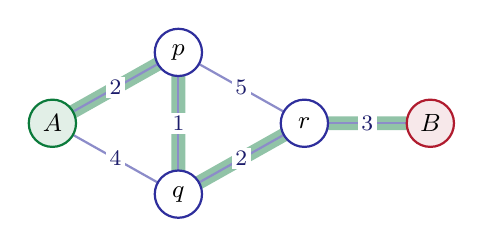
\begin{tikzpicture}[x=1cm, y=1cm]
      \coordinate (A) at (0,0.9);   \coordinate (p) at (1.6,1.8);
      \coordinate (q) at (1.6,0);   \coordinate (r) at (3.2,0.9);
      \coordinate (B) at (4.8,0.9);
      \draw[algastar!45, line width=5pt, line cap=round, line join=round]
        (A) -- (p) -- (q) -- (r) -- (B);
      \foreach \a/\b/\w in {A/p/2, A/q/4, p/q/1, p/r/5, q/r/2, r/B/3}
        {\draw[storyedge] (\a) -- node[storyweight] {\w} (\b);}
      \node[storystart] at (A) {$A$};
      \node[storynode]  at (p) {$p$};
      \node[storynode]  at (q) {$q$};
      \node[storynode]  at (r) {$r$};
      \node[storygoal]  at (B) {$B$};
    \end{tikzpicture}\par\vspace{6pt}
    \caption{A road map. The cheapest route, $(A, p, q, r, B)$,
      costs 8.}\label{fig:pf-graph}
  \end{subfigure}\hfill
  \begin{subfigure}[b]{0.56\textwidth}\centering
    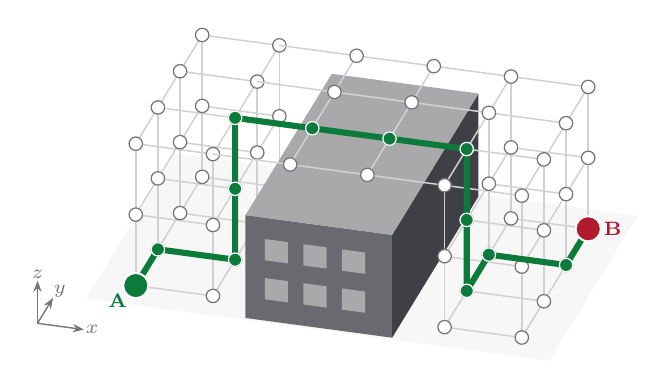
\begin{tikzpicture}[cam={16}{28}{1.02}{1.02}, line cap=round, line join=round]
  \fill[black!3] (-0.5,-0.5,0) -- (5.5,-0.5,0) -- (5.5,3.5,0) -- (-0.5,3.5,0) -- cycle;
  \foreach \y in {0,...,3}{\foreach \z in {0,1,2}{\draw[latedge] (0,\y,\z) -- (1,\y,\z);}}
  \foreach \x in {0,1}{%
    \foreach \z in {0,1,2}{\draw[latedge] (\x,0,\z) -- (\x,3,\z);}
    \foreach \y in {0,...,3}{\draw[latedge] (\x,\y,0) -- (\x,\y,2);}}
  \foreach \x in {0,1}{\foreach \y in {0,...,3}{\foreach \z in {0,1,2}{%
    \node[latnode] at (\x,\y,\z) {};}}}
  \fill[gwall!78!white] (1.55,-0.45,0) -- (3.45,-0.45,0) -- (3.45,-0.45,1.45) -- (1.55,-0.45,1.45) -- cycle;
  \fill[gwall]          (3.45,-0.45,0) -- (3.45,3.45,0)  -- (3.45,3.45,1.45)  -- (3.45,-0.45,1.45) -- cycle;
  \fill[gwall!45!white] (1.55,-0.45,1.45) -- (3.45,-0.45,1.45) -- (3.45,3.45,1.45) -- (1.55,3.45,1.45) -- cycle;
  \foreach \wx in {1.8,2.3,2.8}{\foreach \wz in {0.3,0.85}{%
    \fill[white!55!gwall] (\wx,-0.45,\wz) -- (\wx+0.3,-0.45,\wz)
      -- (\wx+0.3,-0.45,\wz+0.3) -- (\wx,-0.45,\wz+0.3) -- cycle;}}
  \foreach \y in {0,...,3}{\draw[latedge] (1,\y,2) -- (4,\y,2);}
  \foreach \x in {2,3}{\draw[latedge] (\x,0,2) -- (\x,3,2);}
  \foreach \y in {0,...,3}{\foreach \z in {0,1,2}{\draw[latedge] (4,\y,\z) -- (5,\y,\z);}}
  \foreach \x in {4,5}{%
    \foreach \z in {0,1,2}{\draw[latedge] (\x,0,\z) -- (\x,3,\z);}
    \foreach \y in {0,...,3}{\draw[latedge] (\x,\y,0) -- (\x,\y,2);}}
  \foreach \x in {2,3}{\foreach \y in {0,...,3}{\node[latnode] at (\x,\y,2) {};}}
  \foreach \x in {4,5}{\foreach \y in {0,...,3}{\foreach \z in {0,1,2}{%
    \node[latnode] at (\x,\y,\z) {};}}}
  \draw[edgpath]
    (0,0,0) -- (0,1,0) -- (1,1,0) -- (1,1,1) -- (1,1,2) -- (2,1,2)
    -- (3,1,2) -- (4,1,2) -- (4,1,1) -- (4,1,0) -- (4,2,0) -- (5,2,0)
    -- (5,3,0);
  \foreach \p in {(0,1,0),(1,1,0),(1,1,1),(1,1,2),(2,1,2),(3,1,2),
                  (4,1,2),(4,1,1),(4,1,0),(4,2,0),(5,2,0)}{%
    \node[latnode, fill=cbGreen, draw=white] at \p {};}
  \node[sball] at (0,0,0) {};
  \node[tag, text=gstart, below left=2pt] at (0,0,0) {\textbf{A}};
  \node[gball] at (5,3,0) {};
  \node[tag, text=ggoal, right=4pt] at (5,3,0) {\textbf{B}};
  \begin{scope}[shift={(-0.9,-1.3,0)}]
    \draw[-{Stealth[length=1.4mm]}, neutralg, line width=0.5pt] (0,0,0) -- (0.6,0,0)
      node[tag, text=neutralg, right=-1pt] {$x$};
    \draw[-{Stealth[length=1.4mm]}, neutralg, line width=0.5pt] (0,0,0) -- (0,0.7,0)
      node[tag, text=neutralg, above right=-2pt] {$y$};
    \draw[-{Stealth[length=1.4mm]}, neutralg, line width=0.5pt] (0,0,0) -- (0,0,0.6)
      node[tag, text=neutralg, above=-1pt] {$z$};
  \end{scope}
\end{tikzpicture}

    \caption{A three-dimensional lattice. A building removes the points inside
      it, and the cheapest route climbs over the roof.}\label{fig:pf-3d}
  \end{subfigure}
  \caption{Two instances of the pathfinding problem.}\label{fig:pathfinding}
\end{figure}

\subsection{Applications}\label{sec:applications}

Table~\ref{tab:applications} lists typical applications of pathfinding.

\begin{table}[H]
  \centering
  \caption{Applications of pathfinding.}\label{tab:applications}
  \small
  \renewcommand{\arraystretch}{1.25}%
  \begin{tabular}{@{}P{2.5cm}P{2.6cm}P{3.1cm}P{5.6cm}@{}}
    \toprule
    Application & Vertices & Cost of an edge & Example\\
    \midrule
    Road navigation & road junctions & length or travel time of a road
      & planning the fastest drive from Dhaka to Sylhet\\
    Video games & tiles of the map & difficulty of the terrain entered
      & a character that walks around a river to a bridge instead of wading
        through it\\
    Computer networks & routers & delay or load of a link
            & the OSPF protocol\tablefootnote{OSPF (Open Shortest Path First) is the
        routing protocol with which the routers inside one network exchange
        link costs and compute the shortest path to every destination.}, in
        which every router runs Dijkstra's algorithm to choose the paths of data
        packets\\
    Robotics & positions in free space & distance or energy
      & warehouse robots that carry shelves to packing stations without
        colliding\\
    Molecular biology & shapes of a protein & energy needed to change shape
      & the Folding@home project, which searches networks of protein shapes for
        likely folding pathways\\
    Puzzles & board positions & one per move
      & the fewest moves that solve the 15-puzzle or Rubik's
        Cube~\cite{korf1985, korf1997}\\
    \bottomrule
  \end{tabular}
\end{table}

\subsection{The need for pathfinding algorithms}\label{sec:need}

Listing every route and keeping the cheapest is infeasible, because the number
of routes grows exponentially with the size of the map. On a $50 \times 50$
grid there are about $2.5 \times 10^{28}$ routes between opposite corners that
only move right or up; checking a billion per second would take about 800
billion years. Pathfinding algorithms instead grow routes outward from the
source and discard a route as soon as a cheaper route to the same place is
known.

\subsection{Requirements of a pathfinding algorithm}\label{sec:requirements}

A pathfinding algorithm must serve every pair of source and destination, so we
judge it by two requirements.
\begin{description}[font=\normalfont\bfseries, leftmargin=1.5em, labelindent=0pt]
  \item[Optimality.] Whenever the destination can be reached from the source,
    the algorithm returns a cheapest route between them.
  \item[Efficiency.] The algorithm finds this route while examining as little
    of the map as possible.
\end{description}

\section{Preliminaries}\label{sec:prelim}

This section fixes the terminology and notation and introduces the running
example.

\subsection{Graphs and paths}\label{sec:def-graph}

\begin{definition}[Weighted graph]\label{def:graph}
A \emph{weighted graph} $G = (V, E, w)$ consists of a finite set $V$ of
vertices, a set $E$ of edges, each of which joins two vertices, and a weight
function $w$ that assigns a nonnegative cost $w(u,v)$ to every edge $(u,v)$.
\end{definition}

All graphs in this report are undirected. In Figure~\ref{fig:defs},
$V = \{A, p, q, r, B\}$ and $w(A,p) = 2$.

\begin{definition}[Path and path cost]\label{def:path}
A \emph{path} from a vertex $u$ to a vertex $v$ is a sequence of vertices
$P = (v_0, v_1, \dots, v_k)$ with $v_0 = u$ and $v_k = v$ in which every two
consecutive vertices are joined by an edge. The \emph{cost} of the path is
\begin{equation}\label{eq:pathcost}
  c(P) = \sum_{i=1}^{k} w(v_{i-1}, v_i).
\end{equation}
\end{definition}

For example, the path $(A, q, r, B)$ of Figure~\ref{fig:defs-b} costs
$4 + 2 + 3 = 9$.

\begin{definition}[Distance and shortest path]\label{def:shortest}
The \emph{distance} $\delta(u,v)$ from a vertex $u$ to a vertex $v$ is the
minimum cost of a path from $u$ to $v$; if no such path exists, then
$\delta(u,v) = \infty$. A path from $u$ to $v$ of cost $\delta(u,v)$ is a
\emph{shortest path} from $u$ to $v$.
\end{definition}

Table~\ref{tab:defs-paths} lists the paths from $A$ to $B$ that visit no vertex
twice; the shortest one has the most edges.

\begin{figure}[htbp]
  \centering
  \newcommand{\defsgraph}[2]{%
  \begin{tikzpicture}[x=0.9cm, y=0.9cm]
    \coordinate (A) at (0,0.9);   \coordinate (p) at (1.6,1.8);
    \coordinate (q) at (1.6,0);   \coordinate (r) at (3.2,0.9);
    \coordinate (B) at (4.8,0.9);
    \ifx\relax#1\relax\else
      \draw[#2, line width=5pt, line cap=round, line join=round] #1;
    \fi
    \foreach \a/\b/\w in {A/p/2, A/q/4, p/q/1, p/r/5, q/r/2, r/B/3}
      {\draw[storyedge] (\a) -- node[storyweight] {\w} (\b);}
    \node[storystart] at (A) {$A$};
    \node[storynode]  at (p) {$p$};
    \node[storynode]  at (q) {$q$};
    \node[storynode]  at (r) {$r$};
    \node[storygoal]  at (B) {$B$};
  \end{tikzpicture}}
\begin{subfigure}[t]{0.32\textwidth}\centering
  \defsgraph{}{}
  \caption{A weighted graph with five vertices and six edges.}\label{fig:defs-a}
\end{subfigure}\hfill
\begin{subfigure}[t]{0.32\textwidth}\centering
  \defsgraph{(A) -- (q) -- (r) -- (B)}{alggreedy!45}
  \caption{The path $(A,q,r,B)$ has cost $4 + 2 + 3 = 9$.}\label{fig:defs-b}
\end{subfigure}\hfill
\begin{subfigure}[t]{0.32\textwidth}\centering
  \defsgraph{(A) -- (p) -- (q) -- (r) -- (B)}{algastar!45}
  \caption{The shortest path $(A,p,q,r,B)$ has cost $2 + 1 + 2 + 3 = 8$.}\label{fig:defs-c}
\end{subfigure}

  \caption{Paths in the road map of Figure~\ref{fig:pf-graph}.}\label{fig:defs}
\end{figure}

\begin{table}[htbp]
  \centering
  \caption{All paths from $A$ to $B$ in Figure~\ref{fig:defs} that visit no
    vertex twice.}\label{tab:defs-paths}
  \begin{tabular}{@{}lcl@{}}
    \toprule
    Path & Edges & Cost\\
    \midrule
    $(A, p, q, r, B)$ & 4 & $2 + 1 + 2 + 3 = \mathbf{8}$ \quad shortest, $\delta(A,B) = 8$\\
    $(A, q, r, B)$    & 3 & $4 + 2 + 3 = 9$\\
    $(A, p, r, B)$    & 3 & $2 + 5 + 3 = 10$\\
    $(A, q, p, r, B)$ & 4 & $4 + 1 + 5 + 3 = 13$\\
    \bottomrule
  \end{tabular}
\end{table}

\subsection{Heuristic functions}\label{sec:def-heuristic}

A search does not know in advance how far each vertex is from the destination
$t$, but it can use a quick estimate, such as the straight-line distance on a
map. We write $h^{*}(v) = \delta(v,t)$ for the true remaining cost.

\begin{definition}[Heuristic function]\label{def:heuristic}
A \emph{heuristic function}, or simply a \emph{heuristic}, is a function $h$
that assigns to every vertex $v$ a nonnegative number $h(v)$, an estimate of
the remaining cost $h^{*}(v)$.
\end{definition}

\subsection{Best-first search}\label{sec:bestfirst}

All three algorithms of this report are \emph{best-first searches}. They keep a
\emph{priority queue}~\cite{baeldungpq} $Q$ of vertices that have been reached but not explored,
each with a numerical \emph{key}; a smaller key means a more promising vertex.
In each round the search removes a vertex $u$ with the smallest key and
\emph{expands} it: it adds $u$ to the set $S$ of \emph{closed} vertices and
examines every edge $(u,v)$, which may insert $v$ into $Q$ or lower its key.
The search stops when it removes the destination. The algorithms differ only in
the key.

The pseudocode uses three queue operations: \textsc{Extract-Min}$(Q)$ removes
and returns a vertex with the smallest key, \textsc{Insert}$(Q, v, k)$ adds $v$
with key $k$, and \textsc{Insert-or-Decrease-Key}$(Q, v, k)$ adds $v$ or, if it
is already in $Q$, lowers its key to $k$. We measure the work of a search by the
number of vertices it expands, the destination included.
Table~\ref{tab:notation} collects the notation.

\begin{table}[htbp]
  \centering
  \caption{Notation used in the report.}\label{tab:notation}
  \begin{tabular}{@{}ll@{}}
    \toprule
    Symbol & Meaning\\
    \midrule
    $G = (V,E,w)$ & weighted graph with vertex set $V$, edge set $E$ and weights $w$\\
    $s$, $t$      & source vertex and destination vertex\\
    $\delta(u,v)$ & distance from $u$ to $v$, the cost of a shortest path\\
    $C^{*}$       & distance from $s$ to $t$, that is, $\delta(s,t)$\\
    $g(v)$        & cost of the cheapest path from $s$ to $v$ found so far\\
    $h(v)$        & heuristic estimate of the remaining cost from $v$ to $t$\\
    $h^{*}(v)$    & true remaining cost $\delta(v,t)$\\
    $f(v)$        & key used by A*, $f(v) = g(v) + h(v)$\\
    $\pi(v)$      & predecessor of $v$ on the cheapest path found so far\\
    $Q$           & priority queue of vertices reached but not yet expanded\\
    $S$           & set of closed vertices, that is, of expanded vertices\\
    \bottomrule
  \end{tabular}
\end{table}

\subsection{The running example}\label{sec:running}

Figure~\ref{fig:running} shows the graph on which we trace the algorithms:
eight cities from Dhaka (\cty{D}) to Sylhet (\cty{S}), with Gazipur (\cty{G}),
Narsingdi (\cty{N}), Kishoreganj (\cty{K}), Brahmanbaria (\cty{B}), Cumilla
(\cty{C}) and Habiganj (\cty{H}).  The edge weights are small integers
chosen for the example, and each disc shows a heuristic value $h(v)$, which never
exceeds the true remaining cost (Table~\ref{tab:story-h}). The shortest path is
$(\cty{D}, \cty{N}, \cty{B}, \cty{H}, \cty{S})$, of cost $C^{*} = 8$.

\begin{figure}[htbp]
  \centering
  \resizebox{0.62\textwidth}{!}{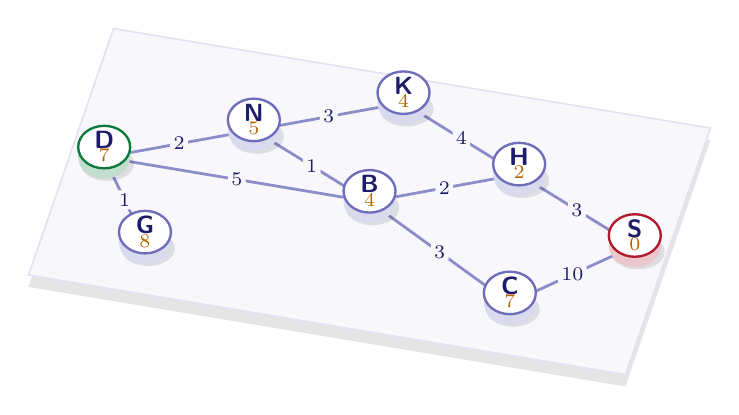
\begin{tikzpicture}[x=1cm, y=1cm]
  \fill[black!10] (-0.529,-0.393) -- (7.052,-1.657) -- (8.132,1.475) -- (0.551,2.739) -- cycle;
  \draw[draw=rblue!14, fill=rbluelt!35, line width=0.6pt] (-0.529,-0.243) -- (7.052,-1.507) -- (8.132,1.625) -- (0.551,2.889) -- cycle;
  \coordinate (D) at (0.432,1.253);
  \coordinate (N) at (2.333,1.598);
  \coordinate (B) at (3.802,0.691);
  \coordinate (H) at (5.702,1.037);
  \coordinate (S) at (7.171,0.130);
  \coordinate (G) at (0.950,0.173);
  \coordinate (K) at (4.234,1.944);
  \coordinate (C) at (5.584,-0.599);
  \draw[draw=rblue!55, line width=1pt] (D) -- (N);
  \draw[draw=rblue!55, line width=1pt] (D) -- (B);
  \draw[draw=rblue!55, line width=1pt] (N) -- (B);
  \draw[draw=rblue!55, line width=1pt] (B) -- (H);
  \draw[draw=rblue!55, line width=1pt] (H) -- (S);
  \draw[draw=rblue!55, line width=1pt] (D) -- (G);
  \draw[draw=rblue!55, line width=1pt] (N) -- (K);
  \draw[draw=rblue!55, line width=1pt] (K) -- (H);
  \draw[draw=rblue!55, line width=1pt] (B) -- (C);
  \draw[draw=rblue!55, line width=1pt] (C) -- (S);
  \node[isoweight] at ($(D)!0.5!(N)$) {2};
  \node[isoweight] at ($(D)!0.5!(B)$) {5};
  \node[isoweight] at ($(N)!0.5!(B)$) {1};
  \node[isoweight] at ($(B)!0.5!(H)$) {2};
  \node[isoweight] at ($(H)!0.5!(S)$) {3};
  \node[isoweight] at ($(D)!0.5!(G)$) {1};
  \node[isoweight] at ($(N)!0.5!(K)$) {3};
  \node[isoweight] at ($(K)!0.5!(H)$) {4};
  \node[isoweight] at ($(B)!0.5!(C)$) {3};
  \node[isoweight] at ($(C)!0.5!(S)$) {10};
  \isodisc{D}{white}{algastar}{D}{7}
  \isodisc{N}{white}{rblue!70}{N}{5}
  \isodisc{B}{white}{rblue!70}{B}{4}
  \isodisc{H}{white}{rblue!70}{H}{2}
  \isodisc{S}{white}{cbRed}{S}{0}
  \isodisc{G}{white}{rblue!70}{G}{8}
  \isodisc{K}{white}{rblue!70}{K}{4}
  \isodisc{C}{white}{rblue!70}{C}{7}
\end{tikzpicture}
}
  \caption{The running example. Each edge shows its weight and each disc the
    heuristic value $h$; the source \cty{D} has a green rim and the destination
    \cty{S} a red rim.}\label{fig:running}
\end{figure}

\begin{table}[htbp]
  \centering
  \caption{The heuristic $h$ of the running example and the true remaining
    cost $h^{*}$.}\label{tab:story-h}
  \begin{tabular}{@{}lcccccccc@{}}
    \toprule
    City & \cty{D} & \cty{G} & \cty{N} & \cty{K} & \cty{B} & \cty{C} & \cty{H} & \cty{S}\\
    \midrule
    Heuristic $h$        & 7 & 8 & 5 & 4 & 4 & 7 & 2 & 0\\
    True cost $h^{*}$    & 8 & 9 & 6 & 7 & 5 & 8 & 3 & 0\\
    \bottomrule
  \end{tabular}
\end{table}

\section{Dijkstra's algorithm and greedy best-first search}
\label{sec:predecessors}

Dijkstra's algorithm~\cite{dijkstra1959} ranks a vertex by the cost already
paid to reach it, and greedy best-first search ranks it by the estimated cost
that remains. Each meets only one of the two requirements of
Section~\ref{sec:requirements}.

\subsection{Dijkstra's algorithm}\label{sec:dijkstra}

Dijkstra's algorithm always expands the waiting vertex that is cheapest to
reach. Its key is $g(v)$, the cost of the cheapest path from the source to $v$
found so far ($0$ at the source and $\infty$ elsewhere at the start). Expanding
$u$ \emph{relaxes} every edge $(u,v)$ with $v$ not closed: if
$g(u) + w(u,v) < g(v)$, the path through $u$ is cheaper, so $g(v)$ is lowered
and $u$ becomes the \emph{predecessor} $\pi(v)$. When the destination is
extracted, following the predecessors back to the source gives the path.
Algorithms~\ref{alg:dijkstra} and~\ref{alg:reconstruct} state the procedure in
the style of Cormen et al.~\cite{cormen2022clrs}.

\begin{algorithm}[htbp]
  \caption{Dijkstra's algorithm}\label{alg:dijkstra}
  \begin{algorithmic}[1]
    \Require graph $G = (V,E,w)$ with nonnegative weights, source $s$, destination $t$
    \Ensure a shortest path from $s$ to $t$, or failure
    \Procedure{Dijkstra}{$G, s, t$}
      \For{each vertex $v$ of $V$}
        \State $g(v) \gets \infty$; \ $\pi(v) \gets \nil$
      \EndFor
      \State $g(s) \gets 0$
      \State $Q \gets$ a priority queue keyed by $g$ that holds $s$
      \State $S \gets \emptyset$
      \While{$Q$ is not empty}
        \State $u \gets \Call{Extract-Min}{Q}$
        \If{$u = t$}
          \State \Return \Call{Reconstruct}{$\pi, t$}
        \EndIf
        \State add $u$ to $S$
        \For{each edge $(u,v)$ such that $v$ is not in $S$}
          \If{$g(u) + w(u,v) < g(v)$}
            \State $g(v) \gets g(u) + w(u,v)$; \ $\pi(v) \gets u$
            \State \Call{Insert-or-Decrease-Key}{$Q, v, g(v)$}
          \EndIf
        \EndFor
      \EndWhile
      \State \Return failure \Comment{$t$ is not reachable from $s$}
    \EndProcedure
  \end{algorithmic}
\end{algorithm}

\begin{algorithm}[htbp]
  \caption{Reconstruction of the path from the predecessors}\label{alg:reconstruct}
  \begin{algorithmic}[1]
    \Require predecessors $\pi$ recorded by a search from $s$, destination $t$
    \Ensure the path from $s$ to $t$ recorded in $\pi$
    \Procedure{Reconstruct}{$\pi, t$}
      \State $P \gets$ an empty list
      \State $v \gets t$
      \While{$v \neq \nil$}
        \State insert $v$ at the front of $P$
        \State $v \gets \pi(v)$ \Comment{step back to the predecessor}
      \EndWhile
      \State \Return $P$ \Comment{$P$ now starts at $s$ and ends at $t$}
    \EndProcedure
  \end{algorithmic}
\end{algorithm}

Table~\ref{tab:trace-dijkstra} traces Algorithm~\ref{alg:dijkstra} on the
running example; each row lists $Q$ in extraction order (by key, ties first in,
first out). The algorithm returns the shortest path of cost 8 but expands all
eight cities (Figure~\ref{fig:story-dijkstra}), including Gazipur, Kishoreganj
and Cumilla, which lie off the path, only because they are cheaper to reach
than Sylhet.

\begin{table}[htbp]
  \centering
  \caption{Dijkstra's algorithm on the running example. The key of a vertex is
    $g$.}\label{tab:trace-dijkstra}
  \small
  \begin{tabular}{@{}c>{\raggedright}P{4.2cm}ccP{4.4cm}@{}}
    \toprule
    Step & $Q$ before extraction (vertex: key) & Extracted & Key & Updates\\
    \midrule
    \inputrows{figures/trace_dijkstra.tex}
    \bottomrule
  \end{tabular}
\end{table}

\begin{remark}[Shortcoming of Dijkstra's algorithm]\label{rem:dijkstra}
The key $g$ ignores where the destination lies, so Dijkstra's algorithm
expands every vertex that is cheaper to reach than the destination, in every
direction (Proposition~\ref{prop:expanded}). It meets the optimality
requirement but not the efficiency requirement.
\end{remark}

\subsection{Greedy best-first search}\label{sec:greedy}

Greedy best-first search uses the key $h(v)$ and always expands the vertex that
looks closest to the destination, whatever it cost to reach. In
Algorithm~\ref{alg:greedy} the predecessor of a vertex is fixed when the vertex
is first reached, so a route, once found, is never improved.

\begin{algorithm}[htbp]
  \caption{Greedy best-first search}\label{alg:greedy}
  \begin{algorithmic}[1]
    \Require graph $G = (V,E,w)$, source $s$, destination $t$, heuristic $h$
    \Ensure a path from $s$ to $t$, or failure
    \Procedure{Greedy-Best-First}{$G, s, t, h$}
      \For{each vertex $v$ of $V$}
        \State $\pi(v) \gets \nil$
      \EndFor
      \State $R \gets \{s\}$ \Comment{vertices reached so far}
      \State $Q \gets$ a priority queue keyed by $h$ that holds $s$
      \While{$Q$ is not empty}
        \State $u \gets \Call{Extract-Min}{Q}$
        \If{$u = t$}
          \State \Return \Call{Reconstruct}{$\pi, t$}
        \EndIf
        \For{each edge $(u,v)$ such that $v$ is not in $R$}
          \State add $v$ to $R$; \ $\pi(v) \gets u$
          \State \Call{Insert}{$Q, v, h(v)$}
        \EndFor
      \EndWhile
      \State \Return failure
    \EndProcedure
  \end{algorithmic}
\end{algorithm}

Table~\ref{tab:trace-greedy} traces it on the running example. It expands only
four cities but returns $(\cty{D}, \cty{B}, \cty{H}, \cty{S})$ of cost 10
instead of 8 (Figure~\ref{fig:story-greedy}). In step 2 it prefers \cty{B}
($h = 4$) to \cty{N} ($h = 5$), ignoring that the direct road to \cty{B} costs 5
while the route through \cty{N} costs 3; since the predecessor of \cty{B} is
already fixed to \cty{D}, the cheaper route is never found.

\begin{table}[htbp]
  \centering
  \caption{Greedy best-first search on the running example. The key of a vertex
    is $h$.}\label{tab:trace-greedy}
  \small
  \begin{tabular}{@{}c>{\raggedright}P{5.4cm}ccP{3.2cm}@{}}
    \toprule
    Step & $Q$ before extraction (vertex: key) & Extracted & Key
      & Vertices reached\\
    \midrule
    \inputrows{figures/trace_greedy.tex}
    \bottomrule
  \end{tabular}
\end{table}

\begin{figure}[htbp]
  \centering
  \begin{subfigure}[b]{0.49\textwidth}\centering
    \resizebox{\linewidth}{!}{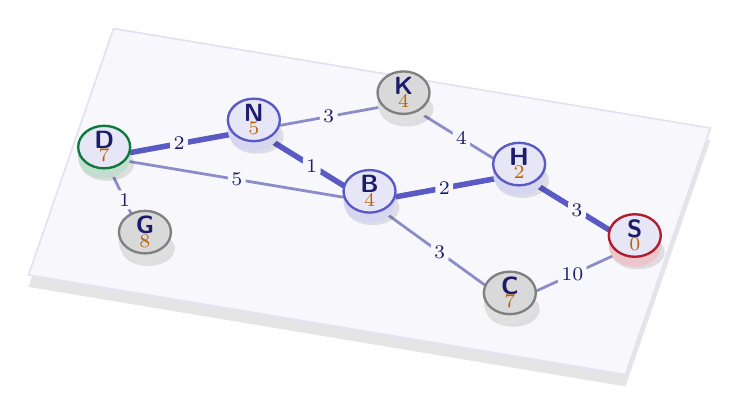
\begin{tikzpicture}[x=1cm, y=1cm]
  \fill[black!10] (-0.529,-0.393) -- (7.052,-1.657) -- (8.132,1.475) -- (0.551,2.739) -- cycle;
  \draw[draw=rblue!14, fill=rbluelt!35, line width=0.6pt] (-0.529,-0.243) -- (7.052,-1.507) -- (8.132,1.625) -- (0.551,2.889) -- cycle;
  \coordinate (D) at (0.432,1.253);
  \coordinate (N) at (2.333,1.598);
  \coordinate (B) at (3.802,0.691);
  \coordinate (H) at (5.702,1.037);
  \coordinate (S) at (7.171,0.130);
  \coordinate (G) at (0.950,0.173);
  \coordinate (K) at (4.234,1.944);
  \coordinate (C) at (5.584,-0.599);
  \draw[draw=algdijkstra, line width=2pt] (D) -- (N);
  \draw[draw=rblue!55, line width=1pt] (D) -- (B);
  \draw[draw=algdijkstra, line width=2pt] (N) -- (B);
  \draw[draw=algdijkstra, line width=2pt] (B) -- (H);
  \draw[draw=algdijkstra, line width=2pt] (H) -- (S);
  \draw[draw=rblue!55, line width=1pt] (D) -- (G);
  \draw[draw=rblue!55, line width=1pt] (N) -- (K);
  \draw[draw=rblue!55, line width=1pt] (K) -- (H);
  \draw[draw=rblue!55, line width=1pt] (B) -- (C);
  \draw[draw=rblue!55, line width=1pt] (C) -- (S);
  \node[isoweight] at ($(D)!0.5!(N)$) {2};
  \node[isoweight] at ($(D)!0.5!(B)$) {5};
  \node[isoweight] at ($(N)!0.5!(B)$) {1};
  \node[isoweight] at ($(B)!0.5!(H)$) {2};
  \node[isoweight] at ($(H)!0.5!(S)$) {3};
  \node[isoweight] at ($(D)!0.5!(G)$) {1};
  \node[isoweight] at ($(N)!0.5!(K)$) {3};
  \node[isoweight] at ($(K)!0.5!(H)$) {4};
  \node[isoweight] at ($(B)!0.5!(C)$) {3};
  \node[isoweight] at ($(C)!0.5!(S)$) {10};
  \isodisc{D}{algdijkstra!15}{algastar}{D}{7}
  \isodisc{N}{algdijkstra!15}{algdijkstra}{N}{5}
  \isodisc{B}{algdijkstra!15}{algdijkstra}{B}{4}
  \isodisc{H}{algdijkstra!15}{algdijkstra}{H}{2}
  \isodisc{S}{algdijkstra!15}{cbRed}{S}{0}
  \isodisc{G}{gray!30}{gray}{G}{8}
  \isodisc{K}{gray!30}{gray}{K}{4}
  \isodisc{C}{gray!30}{gray}{C}{7}
\end{tikzpicture}
}
    \caption{Dijkstra's algorithm expands all eight cities and returns a path of
      cost 8.}\label{fig:story-dijkstra}
  \end{subfigure}\hfill
  \begin{subfigure}[b]{0.49\textwidth}\centering
    \resizebox{\linewidth}{!}{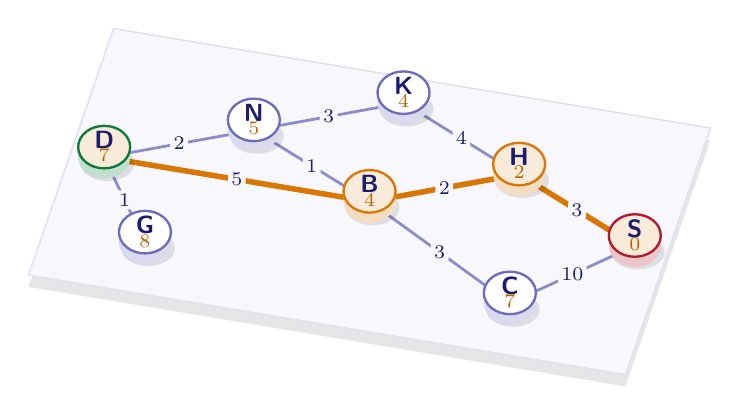
\begin{tikzpicture}[x=1cm, y=1cm]
  \fill[black!10] (-0.529,-0.393) -- (7.052,-1.657) -- (8.132,1.475) -- (0.551,2.739) -- cycle;
  \draw[draw=rblue!14, fill=rbluelt!35, line width=0.6pt] (-0.529,-0.243) -- (7.052,-1.507) -- (8.132,1.625) -- (0.551,2.889) -- cycle;
  \coordinate (D) at (0.432,1.253);
  \coordinate (N) at (2.333,1.598);
  \coordinate (B) at (3.802,0.691);
  \coordinate (H) at (5.702,1.037);
  \coordinate (S) at (7.171,0.130);
  \coordinate (G) at (0.950,0.173);
  \coordinate (K) at (4.234,1.944);
  \coordinate (C) at (5.584,-0.599);
  \draw[draw=rblue!55, line width=1pt] (D) -- (N);
  \draw[draw=alggreedy, line width=2pt] (D) -- (B);
  \draw[draw=rblue!55, line width=1pt] (N) -- (B);
  \draw[draw=alggreedy, line width=2pt] (B) -- (H);
  \draw[draw=alggreedy, line width=2pt] (H) -- (S);
  \draw[draw=rblue!55, line width=1pt] (D) -- (G);
  \draw[draw=rblue!55, line width=1pt] (N) -- (K);
  \draw[draw=rblue!55, line width=1pt] (K) -- (H);
  \draw[draw=rblue!55, line width=1pt] (B) -- (C);
  \draw[draw=rblue!55, line width=1pt] (C) -- (S);
  \node[isoweight] at ($(D)!0.5!(N)$) {2};
  \node[isoweight] at ($(D)!0.5!(B)$) {5};
  \node[isoweight] at ($(N)!0.5!(B)$) {1};
  \node[isoweight] at ($(B)!0.5!(H)$) {2};
  \node[isoweight] at ($(H)!0.5!(S)$) {3};
  \node[isoweight] at ($(D)!0.5!(G)$) {1};
  \node[isoweight] at ($(N)!0.5!(K)$) {3};
  \node[isoweight] at ($(K)!0.5!(H)$) {4};
  \node[isoweight] at ($(B)!0.5!(C)$) {3};
  \node[isoweight] at ($(C)!0.5!(S)$) {10};
  \isodisc{D}{alggreedy!15}{algastar}{D}{7}
  \isodisc{N}{white}{rblue!70}{N}{5}
  \isodisc{B}{alggreedy!15}{alggreedy}{B}{4}
  \isodisc{H}{alggreedy!15}{alggreedy}{H}{2}
  \isodisc{S}{alggreedy!15}{cbRed}{S}{0}
  \isodisc{G}{white}{rblue!70}{G}{8}
  \isodisc{K}{white}{rblue!70}{K}{4}
  \isodisc{C}{white}{rblue!70}{C}{7}
\end{tikzpicture}
}
    \caption{Greedy best-first search expands four cities and returns a path of
      cost 10.}\label{fig:story-greedy}
  \end{subfigure}
  \caption{The two predecessors of A* on the running example. The thick line is
    the returned path; gray discs are expanded cities that are not on
    it.}\label{fig:story-two}
\end{figure}

\begin{remark}[Shortcoming of greedy best-first search]\label{rem:greedy}
The key $h$ ignores the cost already paid. Greedy best-first search meets the
efficiency requirement but not the optimality requirement.
\end{remark}

\subsection{Comparison}\label{sec:side-by-side}

Table~\ref{tab:shortcomings} compares the two algorithms; each has the
strength that the other lacks.

\begin{table}[htbp]
  \centering
  \caption{Dijkstra's algorithm and greedy best-first search compared on the
    running example.}\label{tab:shortcomings}
  \renewcommand{\arraystretch}{1.25}%
  \begin{tabular}{@{}P{4.4cm}P{4.6cm}P{4.6cm}@{}}
    \toprule
     & \textcolor{algdijkstra}{\textbf{Dijkstra's algorithm}}
     & \textcolor{alggreedy}{\textbf{Greedy best-first search}}\\
    \midrule
    Key of a vertex $v$     & $g(v)$, the cost so far & $h(v)$, the estimated
                              remaining cost\\
    Uses the position of the destination & no  & yes\\
    Replaces a found route by a cheaper one & yes & no\\
    Cities expanded         & 8 of 8 & 4 of 8\\
    Cost of the returned path & 8 (optimal) & 10\\
    Optimality requirement  & \textcolor{algastar}{met} & \textcolor{cbRed}{not met}\\
    Efficiency requirement  & \textcolor{cbRed}{not met} & \textcolor{algastar}{met}\\
    \bottomrule
  \end{tabular}
\end{table}

\section{The A* algorithm}\label{sec:astar}

A*~\cite{hart1968formal} keeps the cost so far of Dijkstra's algorithm and adds
the estimate of greedy best-first search (Figure~\ref{fig:combine}).

\begin{figure}[htbp]
  \centering
  \tikzset{
  card/.style  = {draw=#1, fill=#1!9, line width=0.9pt, rounded corners=3pt,
                  text width=4.8cm, align=center, font=\small, inner sep=6pt},
  cflow/.style = {-{Stealth[length=2.4mm]}, line width=1pt, draw=inkgray},
  cflab/.style = {font=\small, text=inkgray, fill=white, inner sep=2pt},
}
\begin{tikzpicture}[x=1cm, y=1cm]
  \node[card=algdijkstra] (dj) at (-3.4,1.7)
    {\textcolor{algdijkstra}{\textbf{Dijkstra's algorithm}}\\[2pt]
     ranks by $g$, the cost so far\\[3pt]
     \textcolor{algastar}{$\checkmark$} shortest path\\
     \textcolor{cbRed}{$\times$} expands all eight cities};
  \node[card=alggreedy] (gr) at (3.4,1.7)
    {\textcolor{alggreedy}{\textbf{Greedy best-first search}}\\[2pt]
     ranks by $h$, the estimate of what is left\\[3pt]
     \textcolor{algastar}{$\checkmark$} expands four cities\\
     \textcolor{cbRed}{$\times$} path cost 10, optimum 8};
  \node[card=algastar, line width=1.3pt, text width=5cm] (as) at (0,-1.6)
    {\textcolor{algastar}{\textbf{A* search}}\\[2pt]
     ranks by $f = g + h$\\[3pt]
     \textcolor{algastar}{$\checkmark$} shortest path (cost 8)\\
     \textcolor{algastar}{$\checkmark$} expands five cities};
  \draw[cflow] (dj.south) -- node[cflab] {keep $g$} ($(as.north)+(-1.2,0)$);
  \draw[cflow] (gr.south) -- node[cflab] {add $h$} ($(as.north)+(1.2,0)$);
\end{tikzpicture}

  \caption{A* takes the cost so far $g$ from Dijkstra's algorithm and the
    estimate $h$ from greedy best-first search. The numbers are those of the
    running example.}\label{fig:combine}
\end{figure}

\subsection{Combining the two keys}\label{sec:fgh}

A* ranks every vertex $v$ of $Q$ by
\begin{equation}\label{eq:f}
  f(v) = g(v) + h(v),
\end{equation}
the estimated cost of the cheapest complete route through $v$
(Figure~\ref{fig:fgh}). A* thus prefers the vertex on the most promising
complete route, rather than the vertex nearest the source or the one that looks
nearest the destination (Table~\ref{tab:three-keys}).

\begin{figure}[htbp]
  \centering
  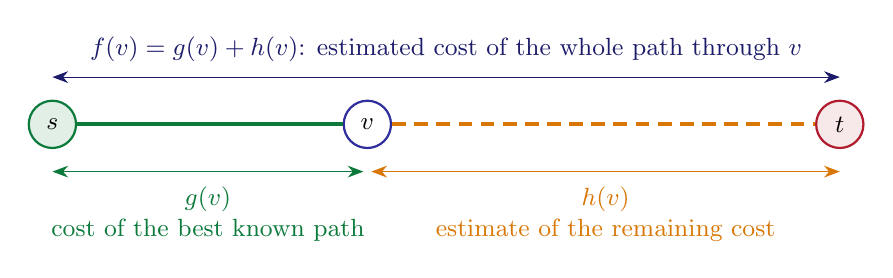
\begin{tikzpicture}[x=1cm, y=1cm]
    \node[storystart] (S) at (0,0) {$s$};
    \node[storynode]  (V) at (4,0) {$v$};
    \node[storygoal]  (T) at (10,0) {$t$};
    \draw[algastar, line width=1.4pt] (S) -- (V);
    \draw[alggreedy, line width=1.4pt, dash pattern=on 5pt off 3pt] (V) -- (T);
    \draw[algastar, {Stealth[length=2mm]}-{Stealth[length=2mm]}]
      (0,-0.6) -- node[below=2pt, font=\small, align=center] {$g(v)$\\cost of
      the best known path} (3.95,-0.6);
    \draw[alggreedy, {Stealth[length=2mm]}-{Stealth[length=2mm]}]
      (4.05,-0.6) -- node[below=2pt, font=\small, align=center] {$h(v)$\\
      estimate of the remaining cost} (10,-0.6);
    \draw[rbluedk, {Stealth[length=2mm]}-{Stealth[length=2mm]}]
      (0,0.6) -- node[above=2pt, font=\small] {$f(v) = g(v) + h(v)$:
      estimated cost of the whole path through $v$} (10,0.6);
  \end{tikzpicture}
  \caption{The key of A*. The first part is known exactly; the second part is
    an estimate.}\label{fig:fgh}
\end{figure}

\begin{table}[htbp]
  \centering
  \caption{The key of each algorithm.}\label{tab:three-keys}
  \begin{tabular}{@{}lll@{}}
    \toprule
    Algorithm & Key of $v$ & What the key measures\\
    \midrule
    Dijkstra's algorithm     & $g(v)$        & the cost already paid\\
    Greedy best-first search & $h(v)$        & the estimated cost still to pay\\
    A* search                & $g(v) + h(v)$ & the estimated cost of the whole path\\
    \bottomrule
  \end{tabular}
\end{table}

\subsection{A geometric view of the key}\label{sec:geometry}

On an open plane, let $g$ be the distance from $s$ and $h$ the distance to $t$.
Then $g$ and $h$ are cones around $s$ and $t$, and their sum $f$ is a trough
whose floor is the segment from $s$ to $t$ (Figure~\ref{fig:surfaces}). A*
therefore expands the points near this segment first.

\begin{figure}[htbp]
  \centering
  \resizebox{\linewidth}{!}{\def\kD{0.45}\def\sgx{1.6}
\newcommand{\surfone}[4]{%
  \begin{tikzpicture}
    \begin{axis}[land3d, land view={-28}{30}{0.52}, colormap name=#1,
                 point meta min=0, point meta max=3.6,
                 xmin=-3.2, xmax=3.2, ymin=-2, ymax=2, zmin=0, zmax=3.6]
      \draw[gridgray, line width=0.4pt] (-3.2,-2,0) -- (3.2,-2,0)
        -- (3.2,2,0) -- (-3.2,2,0) -- cycle;
      \addplot3[tilesurf, domain=-3.2:3.2, y domain=-2:2,
                samples=17, samples y=11] {#2};
      \path (-3.2,-2,3.6) (3.2,-2,3.6) (3.2,2,3.6) (-3.2,2,3.6);
      \node[sball, minimum size=2.6mm] at (-\sgx,0,#3) {};
      \node[gball, minimum size=2.6mm] at (\sgx,0,#4) {};
    \end{axis}
  \end{tikzpicture}}
\begin{tabular}{@{}c@{\hspace{2pt}}c@{\hspace{2pt}}c@{\hspace{2pt}}c@{\hspace{2pt}}c@{}}
  \surfone{hblue}{\kD*veclen(x+\sgx,y)}{0}{\kD*2*\sgx}
  & \raisebox{1.2cm}{\Large $+$}
  & \surfone{horange}{\kD*veclen(x-\sgx,y)}{\kD*2*\sgx}{0}
  & \raisebox{1.2cm}{\Large $=$}
  & \begin{tikzpicture}
      \begin{axis}[land3d, land view={-28}{30}{0.52}, colormap name=hgreen,
                   point meta min=0, point meta max=3.6,
                   xmin=-3.2, xmax=3.2, ymin=-2, ymax=2, zmin=0, zmax=3.6]
        \draw[gridgray, line width=0.4pt] (-3.2,-2,0) -- (3.2,-2,0)
          -- (3.2,2,0) -- (-3.2,2,0) -- cycle;
        \addplot3[tilesurf, domain=-3.2:3.2, y domain=-2:2,
                  samples=17, samples y=11]
          {\kD*(veclen(x+\sgx,y)+veclen(x-\sgx,y))};
        \path (-3.2,-2,3.6) (3.2,-2,3.6) (3.2,2,3.6) (-3.2,2,3.6);
        \draw[cbGreen!60!black, line width=1.8pt]
          (-\sgx,0,{\kD*2*\sgx}) -- (\sgx,0,{\kD*2*\sgx});
        \node[sball, minimum size=2.6mm] at (-\sgx,0,{\kD*2*\sgx}) {};
        \node[gball, minimum size=2.6mm] at (\sgx,0,{\kD*2*\sgx}) {};
      \end{axis}
    \end{tikzpicture}\\
  {\footnotesize\textcolor{rblue}{$g$}: cost so far} &
  & {\footnotesize\textcolor{cbOrange}{$h$}: estimate of what is left} &
  & {\footnotesize\textcolor{cbGreen}{$f = g + h$}}\\
  {\scriptsize\textcolor{neutralg}{Dijkstra: a cone at $s$}} &
  & {\scriptsize\textcolor{neutralg}{greedy: a cone at $t$}} &
  & {\scriptsize\textcolor{neutralg}{A*: a trough from $s$ to $t$}}
\end{tabular}
}
  \caption{The keys as surfaces over a plane: a cone around $s$, a cone around
    $t$, and their sum, a trough whose floor is the segment from $s$ to
    $t$.}\label{fig:surfaces}
\end{figure}

\subsection{Pseudocode}\label{sec:astar-alg}

Algorithm~\ref{alg:astar} is Algorithm~\ref{alg:dijkstra} with the key $g$
replaced by $g + h$ in the two lines marked ``changed''. With the \emph{zero
heuristic}, $h(v) = 0$ for every $v$, it is exactly Dijkstra's algorithm.
Figure~\ref{fig:astar-flow} shows the loop shared by the three algorithms.

\begin{algorithm}[htbp]
  \caption{A* search}\label{alg:astar}
  \begin{algorithmic}[1]
    \Require graph $G = (V,E,w)$ with nonnegative weights, source $s$, destination $t$,
      heuristic $h$
    \Ensure a path from $s$ to $t$, or failure
    \Procedure{A-Star}{$G, s, t, h$}
      \For{each vertex $v$ of $V$}
        \State $g(v) \gets \infty$; \ $\pi(v) \gets \nil$
      \EndFor
      \State $g(s) \gets 0$
      \State $Q \gets$ a priority queue keyed by $g + h$ that holds $s$
        \Comment{changed}
      \State $S \gets \emptyset$
      \While{$Q$ is not empty}
        \State $u \gets \Call{Extract-Min}{Q}$
        \If{$u = t$}
          \State \Return \Call{Reconstruct}{$\pi, t$}
        \EndIf
        \State add $u$ to $S$
        \For{each edge $(u,v)$ such that $v$ is not in $S$}
          \If{$g(u) + w(u,v) < g(v)$}
            \State $g(v) \gets g(u) + w(u,v)$; \ $\pi(v) \gets u$
            \State \Call{Insert-or-Decrease-Key}{$Q, v, g(v) + h(v)$}
              \Comment{changed}
          \EndIf
        \EndFor
      \EndWhile
      \State \Return failure
    \EndProcedure
  \end{algorithmic}
\end{algorithm}

\begin{figure}[htbp]
  \centering
  \tikzset{
  fstep/.style  = {draw=rblue, fill=rbluelt, line width=0.7pt, rounded corners=2pt,
                   text width=6.2cm, align=center, font=\small, inner sep=4pt},
  fterm/.style  = {fstep, fill=rblue, text=white, rounded corners=8pt,
                   text width=2.6cm, font=\small\bfseries},
  fdec/.style   = {draw=alggreedy, fill=alggreedy!12, line width=0.7pt, diamond,
                   aspect=2.4, align=center, font=\small, inner sep=1pt},
  fout/.style   = {fstep, text width=3.2cm},
  farr/.style   = {-{Stealth[length=2mm]}, line width=0.8pt, draw=rbluedk},
  flab/.style   = {font=\scriptsize\bfseries, text=rbluedk, inner sep=2pt},
}
\begin{tikzpicture}[node distance=0.55cm]
  \node[fterm] (start) {Start};
  \node[fstep, below=of start] (init) {$g(s) \gets 0$, every other $g(v) \gets \infty$\\
    $Q \gets \{s\}$, \ $S \gets \emptyset$};
  \node[fdec, below=of init] (empty) {Is $Q$\\empty?};
  \node[fstep, below=of empty] (pop) {$u \gets$ the vertex of $Q$ with the\\
    smallest key};
  \node[fdec, below=of pop] (goal) {$u = t$?};
  \node[fstep, below=of goal] (close) {add $u$ to $S$};
  \node[fstep, below=of close] (relax) {for each edge $(u,v)$ with $v$ not in $S$:\\
    if $g(u) + w(u,v) < g(v)$, then set $g(v)$ and $\pi(v) \gets u$,\\
    and update the key of $v$ in $Q$};
  \node[fout, right=1.4cm of empty] (fail) {return failure};
  \node[fout, fill=algastar!12, draw=algastar, right=1.4cm of goal] (done)
    {\textsc{Reconstruct}$(\pi,t)$\\(Algorithm~\ref{alg:reconstruct})};
  \draw[farr] (start) -- (init);
  \draw[farr] (init) -- (empty);
  \draw[farr] (empty) -- node[flab, right] {no} (pop);
  \draw[farr] (empty) -- node[flab, above] {yes} (fail);
  \draw[farr] (pop) -- (goal);
  \draw[farr] (goal) -- node[flab, above] {yes} (done);
  \draw[farr] (goal) -- node[flab, right] {no} (close);
  \draw[farr] (close) -- (relax);
  \draw[farr] (relax.west) -- ++(-0.7,0) |- (empty.west);
  \node[draw=cbRed, fill=cbRed!6, line width=0.7pt, rounded corners=2pt,
        text width=3.6cm, font=\small, align=left, inner sep=5pt,
        right=1.0cm of relax] (key)
    {\textbf{key of $v$}\\[2pt]
     Dijkstra: \ $g(v)$\\
     greedy: \ $h(v)$\\
     A*: \ $g(v) + h(v)$};
  \draw[cbRed, line width=0.7pt, dashed] (key.west) -- (relax.east);
  \draw[cbRed, line width=0.7pt, dashed] (key.north) |- (pop.east);
\end{tikzpicture}

  \caption{Flow chart of the search loop. The three algorithms differ only in
    the key of a vertex (red box).}\label{fig:astar-flow}
\end{figure}

\subsection{A* on the running example}\label{sec:worked}

Table~\ref{tab:trace-h} and Figure~\ref{fig:story} show A* on the running
example. In step 2, A* expands \cty{N} (key $2 + 5 = 7$) rather than \cty{G}
(key $1 + 8 = 9$), which Dijkstra's algorithm would take first. The same step
lowers $g(\cty{B})$ from 5 to 3 through \cty{N}, repairing the error of greedy
best-first search. In step 5 the destination is extracted with $g = 8$, and
\cty{G}, \cty{K} and \cty{C}, whose keys exceed 8, are never expanded. A* thus
finds the shortest path with five expansions instead of eight.
Sections~\ref{sec:heuristics} and~\ref{sec:correctness} show when this result is
guaranteed, and Section~\ref{sec:efficiency} explains the saving.

\begin{table}[htbp]
  \centering
  \caption{A* on the running example. The key of a vertex is
    $f = g + h$.}\label{tab:trace-h}
  \small
  \begin{tabular}{@{}c>{\raggedright}P{4.4cm}cc>{\raggedright\arraybackslash}P{3.8cm}@{}}
    \toprule
    Step & $Q$ before extraction (vertex: key) & Extracted & $g + h = f$
      & Updates\\
    \midrule
    \inputrows{figures/trace_original.tex}
    \bottomrule
  \end{tabular}
\end{table}

\begin{figure}[htbp]
  \centering
  \resizebox{0.62\textwidth}{!}{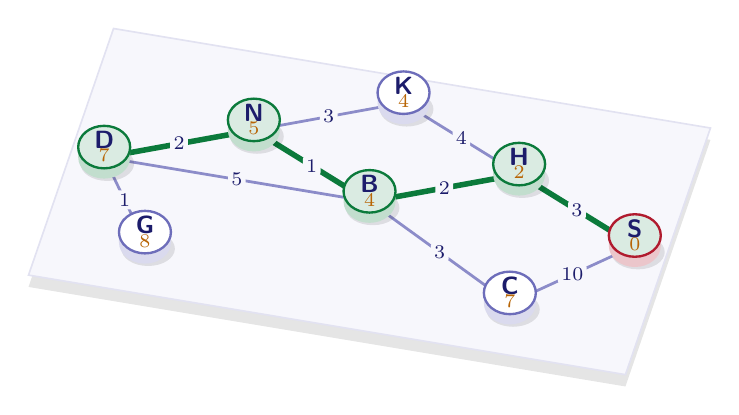
\begin{tikzpicture}[x=1cm, y=1cm]
  \fill[black!10] (-0.529,-0.393) -- (7.052,-1.657) -- (8.132,1.475) -- (0.551,2.739) -- cycle;
  \draw[draw=rblue!14, fill=rbluelt!35, line width=0.6pt] (-0.529,-0.243) -- (7.052,-1.507) -- (8.132,1.625) -- (0.551,2.889) -- cycle;
  \coordinate (D) at (0.432,1.253);
  \coordinate (N) at (2.333,1.598);
  \coordinate (B) at (3.802,0.691);
  \coordinate (H) at (5.702,1.037);
  \coordinate (S) at (7.171,0.130);
  \coordinate (G) at (0.950,0.173);
  \coordinate (K) at (4.234,1.944);
  \coordinate (C) at (5.584,-0.599);
  \draw[draw=algastar, line width=2pt] (D) -- (N);
  \draw[draw=rblue!55, line width=1pt] (D) -- (B);
  \draw[draw=algastar, line width=2pt] (N) -- (B);
  \draw[draw=algastar, line width=2pt] (B) -- (H);
  \draw[draw=algastar, line width=2pt] (H) -- (S);
  \draw[draw=rblue!55, line width=1pt] (D) -- (G);
  \draw[draw=rblue!55, line width=1pt] (N) -- (K);
  \draw[draw=rblue!55, line width=1pt] (K) -- (H);
  \draw[draw=rblue!55, line width=1pt] (B) -- (C);
  \draw[draw=rblue!55, line width=1pt] (C) -- (S);
  \node[isoweight] at ($(D)!0.5!(N)$) {2};
  \node[isoweight] at ($(D)!0.5!(B)$) {5};
  \node[isoweight] at ($(N)!0.5!(B)$) {1};
  \node[isoweight] at ($(B)!0.5!(H)$) {2};
  \node[isoweight] at ($(H)!0.5!(S)$) {3};
  \node[isoweight] at ($(D)!0.5!(G)$) {1};
  \node[isoweight] at ($(N)!0.5!(K)$) {3};
  \node[isoweight] at ($(K)!0.5!(H)$) {4};
  \node[isoweight] at ($(B)!0.5!(C)$) {3};
  \node[isoweight] at ($(C)!0.5!(S)$) {10};
  \isodisc{D}{algastar!15}{algastar}{D}{7}
  \isodisc{N}{algastar!15}{algastar}{N}{5}
  \isodisc{B}{algastar!15}{algastar}{B}{4}
  \isodisc{H}{algastar!15}{algastar}{H}{2}
  \isodisc{S}{algastar!15}{cbRed}{S}{0}
  \isodisc{G}{white}{rblue!70}{G}{8}
  \isodisc{K}{white}{rblue!70}{K}{4}
  \isodisc{C}{white}{rblue!70}{C}{7}
\end{tikzpicture}
}
  \caption{A* on the running example. The green path is the path that A*
    returns, and its cities are exactly the cities that A*
    expands.}\label{fig:story}
\end{figure}

\section{Heuristic functions}\label{sec:heuristics}

The heuristic is the only application-specific part of A*. This section defines
the conditions under which A* is correct, presents the distance heuristics of
our experiments, and shows how a heuristic guides or misleads the search.

\subsection{Requirements}\label{sec:h-requirements}

A good heuristic $h$ meets three requirements.
\begin{enumerate}[label=(\roman*)]
    \item \textbf{It is cheap to compute}, because A* computes it for every
    vertex it reaches.
  \item \textbf{It never overestimates}: $h(v) \le h^{*}(v)$ for every $v$. This
    makes A* return a shortest path (Section~\ref{sec:correctness}).
  \item \textbf{It is close to $h^{*}$}, because larger values leave fewer
    vertices for A* to expand (Section~\ref{sec:efficiency}).
\end{enumerate}
The best heuristic is therefore as large as possible without exceeding the
true cost.

\subsection{Admissible heuristics}\label{sec:admissible}

Requirement~(ii) is called admissibility.

\begin{definition}[Admissible heuristic]\label{def:admissible}
A heuristic $h$ is \emph{admissible} if $0 \le h(v) \le h^{*}(v)$ for every
vertex $v$.
\end{definition}

An admissible heuristic is optimistic. The heuristic of the running example
is admissible (Table~\ref{tab:story-h}); Section~\ref{sec:overestimate} gives
one that is not. At the destination an admissible heuristic is zero, since
$0 \le h(t) \le h^{*}(t) = 0$.

\subsection{Consistent heuristics}\label{sec:consistent}

Algorithm~\ref{alg:astar} needs a stronger condition.

\begin{definition}[Consistent heuristic]\label{def:consistent}
A heuristic $h$ is \emph{consistent} if $h(t) = 0$ and
\begin{equation}\label{eq:consistent}
  h(u) \le w(u,v) + h(v)
\end{equation}
for every edge $(u,v)$.
\end{definition}

In words, one step lowers the estimate by at most the cost of that step, a
triangle inequality (Figure~\ref{fig:consistency}). On undirected graphs it must
hold in both directions of every edge. The heuristic of the running example is
consistent; for instance, $h(\cty{N}) = 5 = w(\cty{N}, \cty{B}) + h(\cty{B})$.

\begin{figure}[htbp]
  \centering
  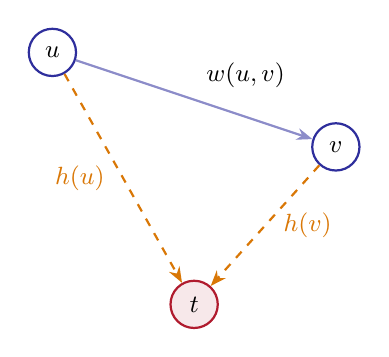
\begin{tikzpicture}[x=1cm, y=1cm]
    \node[storynode] (u) at (0,1.4) {$u$};
    \node[storynode] (v) at (3.6,0.2) {$v$};
    \node[storygoal] (t) at (1.8,-1.8) {$t$};
    \draw[storyedge, -{Stealth[length=2mm]}] (u) -- node[above right=1pt,
      font=\small] {$w(u,v)$} (v);
    \draw[alggreedy, line width=0.8pt, dashed, -{Stealth[length=2mm]}] (v) --
      node[right=3pt, font=\small] {$h(v)$} (t);
    \draw[alggreedy, line width=0.8pt, dashed, -{Stealth[length=2mm]}] (u) --
      node[left=3pt, font=\small] {$h(u)$} (t);
  \end{tikzpicture}
  \caption{Consistency as a triangle inequality: $h(u) \le w(u,v) + h(v)$ for
    every edge $(u,v)$.}\label{fig:consistency}
\end{figure}

Consistency is the stronger condition.

\begin{lemma}\label{lem:cons-adm}
Every consistent heuristic is admissible.
\end{lemma}

\begin{proof}
Let $h$ be a consistent heuristic. By Definition~\ref{def:heuristic}, $h$
takes nonnegative values, so it remains to show that $h(v) \le h^{*}(v)$ for
every vertex $v$. If $t$ is not reachable from $v$, then $h^{*}(v) = \infty$
and there is nothing to prove. Otherwise let $(v = u_0, u_1, \dots, u_m = t)$ be a shortest path from
$v$ to $t$. We show by induction on $m - i$ that
$h(u_i) \le \delta(u_i, t)$. For $i = m$ we have $h(t) = 0 = \delta(t,t)$. For
$i < m$, Inequality~\eqref{eq:consistent} and the induction hypothesis give
\[
  h(u_i) \le w(u_i, u_{i+1}) + h(u_{i+1})
         \le w(u_i, u_{i+1}) + \delta(u_{i+1}, t) = \delta(u_i, t),
\]
where the last equality holds because every part of a shortest path is itself a
shortest path. For $i = 0$ this is $h(v) \le h^{*}(v)$.
\end{proof}

The converse is false; Example~\ref{ex:inconsistent} gives an admissible
heuristic that is not consistent.

\subsection{Distance heuristics}\label{sec:distance-h}

On maps and grids the usual heuristics are distances between the coordinates
of a vertex $v = (x_v, y_v)$ and of the destination $t = (x_t, y_t)$.

\begin{definition}[Manhattan and Euclidean distance]\label{def:distances}
The \emph{Manhattan distance} and the \emph{Euclidean distance} from $v$ to $t$
are
\begin{align}
  h_{M}(v) &= |x_v - x_t| + |y_v - y_t|, \label{eq:manhattan}\\
  h_{E}(v) &= \sqrt{(x_v - x_t)^2 + (y_v - y_t)^2}, \label{eq:euclidean}
\end{align}
respectively. In three dimensions each formula gains a term for the third
coordinate.
\end{definition}

The Manhattan distance follows the axes, like a car on a street grid; the
Euclidean distance is the straight line. For a displacement of $(4, 3, 2)$ they
are 9 and $\sqrt{29} \approx 5.39$ (Figure~\ref{fig:euclid-box}). As surfaces
around the destination they form a pyramid and a cone
(Figure~\ref{fig:cone-pyramid}), and the pyramid never lies below the cone.

\begin{figure}[htbp]
  \centering
  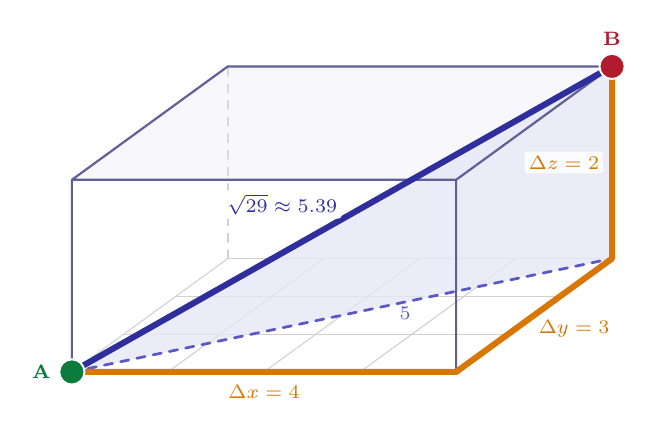
\begin{tikzpicture}[x={(1.22cm,0cm)}, y={(0.66cm,0.48cm)},
                    z={(0cm,1.22cm)}, line join=round, line cap=round]
  \foreach \i in {0,...,4}{\draw[gridgray, line width=0.4pt] (\i,0,0) -- (\i,3,0);}
  \foreach \j in {0,...,3}{\draw[gridgray, line width=0.4pt] (0,\j,0) -- (4,\j,0);}
  \draw[gridgray, dashed, line width=0.6pt] (0,3,0) -- (0,3,2);
  \fill[rbluelt, opacity=0.8] (0,0,0) -- (4,3,0) -- (4,3,2) -- cycle;
  \draw[rbluemd, dashed, line width=1pt] (0,0,0) -- (4,3,0)
    node[pos=0.6, below right=-1pt, tag, text=rbluemd] {$5$};
  \fill[rbluelt, opacity=0.35] (0,0,2) -- (4,0,2) -- (4,3,2) -- (0,3,2) -- cycle;
  \draw[rbluedk!70, line width=0.8pt]
    (0,0,0) -- (4,0,0) -- (4,0,2) -- (0,0,2) -- cycle
    (4,0,0) -- (4,3,0) -- (4,3,2) -- (4,0,2)
    (0,0,2) -- (0,3,2) -- (4,3,2);
  \draw[cbOrange, line width=2.2pt] (0,0,0) -- (4,0,0) -- (4,3,0) -- (4,3,2);
  \node[tag, text=cbOrange, below=3pt] at (2,0,0) {$\Delta x = 4$};
  \node[tag, text=cbOrange, below right=0pt] at (4,1.5,0) {$\Delta y = 3$};
  \node[tagbox, text=cbOrange, left=3pt] at (4,3,1) {$\Delta z = 2$};
  \draw[rblue, line width=2.2pt] (0,0,0) -- (4,3,2);
  \node[tagbox, text=rblue, above left=0pt] at (2,1.5,1) {$\sqrt{29}\approx 5.39$};
  \node[sball] at (0,0,0) {};
  \node[tag, text=gstart, left=6pt] at (0,0,0) {\textbf{A}};
  \node[gball] at (4,3,2) {};
  \node[tag, text=ggoal, above=6pt] at (4,3,2) {\textbf{B}};
\end{tikzpicture}

  \caption{The Manhattan distance (orange, along the edges of the box) and the
    Euclidean distance (blue, straight through the box) from $A$ to
    $B$.}\label{fig:euclid-box}
\end{figure}

\begin{figure}[htbp]
  \centering
  \begin{tabular}{@{}c@{\hspace{1.5em}}c@{}}
  {\footnotesize\textcolor{rblue}{\textbf{Euclidean}} $h=\sqrt{x^2+y^2}$: a cone} &
  {\footnotesize\textcolor{cbOrange}{\textbf{Manhattan}} $h=|x|+|y|$: a pyramid}\\[2pt]
  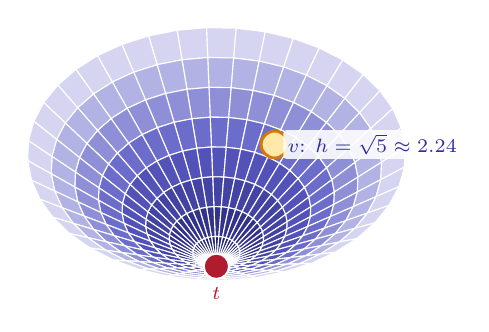
\begin{tikzpicture}
    \begin{axis}[land3d, land view={-30}{42}{0.60},
                 colormap name=hblue, point meta min=0, point meta max=3.2]
      \addplot3[tilesurf, domain=0:4, y domain=0:360, samples=9, samples y=41]
        ({x*cos(y)}, {x*sin(y)}, {\kE*x});
      \node[gball] at (0,0,0) {};
      \node[tag, text=ggoal, below=6pt] at (0,0,0) {$t$};
      \node[vball] at (\pEx,\pEy,{\kE*veclen(\pEx,\pEy)}) {};
      \node[tagbox, text=rblue, anchor=west, right=3pt]
        at (\pEx,\pEy,{\kE*veclen(\pEx,\pEy)}) {$v$: $h=\sqrt5\approx2.24$};
    \end{axis}
  \end{tikzpicture}
  &
  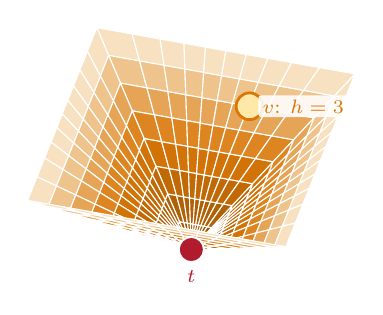
\begin{tikzpicture}
    \begin{axis}[land3d, land view={-30}{42}{0.60},
                 colormap name=horange, point meta min=0, point meta max=3.2]
      \addplot3[tilesurf, domain=0:4, y domain=0:360, samples=9, samples y=41]
        ({x*cos(y)/(abs(cos(y))+abs(sin(y)))},
         {x*sin(y)/(abs(cos(y))+abs(sin(y)))}, {\kE*x});
      \node[gball] at (0,0,0) {};
      \node[tag, text=ggoal, below=6pt] at (0,0,0) {$t$};
      \node[vball] at (\pEx,\pEy,{\kE*(abs(\pEx)+abs(\pEy))}) {};
      \node[tagbox, text=cbOrange, anchor=west, right=3pt]
        at (\pEx,\pEy,{\kE*(abs(\pEx)+abs(\pEy))}) {$v$: $h=3$};
    \end{axis}
  \end{tikzpicture}\\
  {\scriptsize level sets are circles} & {\scriptsize level sets are diamonds}
\end{tabular}

  \caption{The two distance heuristics as surfaces around the destination $t$. At the
    point $v$ with offset $(2,1)$ from $t$ the pyramid is higher: 3 against
    $\sqrt{5} \approx 2.24$.}\label{fig:cone-pyramid}
\end{figure}

\begin{proposition}\label{prop:manh-eucl}
For any two points $v$ and $t$ of the plane, $h_{E}(v) \le h_{M}(v)$, with
equality if and only if $v$ and $t$ agree in at least one coordinate.
\end{proposition}

\begin{proof}
Let $a = |x_v - x_t|$ and $b = |y_v - y_t|$. Both distances are nonnegative, so
it suffices to compare their squares. We have
$h_{M}(v)^2 = (a+b)^2 = a^2 + b^2 + 2ab = h_{E}(v)^2 + 2ab$. Since
$2ab \ge 0$, it follows that $h_{E}(v) \le h_{M}(v)$, with equality exactly when
$ab = 0$, that is, when $a = 0$ or $b = 0$.
\end{proof}

Table~\ref{tab:which-h} shows where each distance is admissible. On a unit-cost
grid with four neighbors per cell, the Manhattan distance equals the true number
of moves when no obstacle intervenes. With straight-line edge weights, no chain
of edges is shorter than the straight line, so the straight-line distance is
admissible, while the larger Manhattan distance may overestimate.

\begin{table}[htbp]
  \centering
  \caption{When a distance heuristic never overestimates.}\label{tab:which-h}
  \renewcommand{\arraystretch}{1.25}%
  \begin{tabular}{@{}P{5.4cm}P{3.6cm}P{4.6cm}@{}}
    \toprule
    Graph & Admissible heuristic & Reason\\
    \midrule
    Grid with four neighbors per cell, every move of cost 1
      (Section~\ref{sec:grid})
      & Manhattan distance & every move changes one coordinate by 1\\
    Edge weights equal to straight-line distances
      (Section~\ref{sec:mapgraph})
      & Euclidean or great-circle distance & no chain of edges is shorter
        than the direct line\\
    Edge weights unrelated to the coordinates
      (Section~\ref{sec:overestimate})
      & neither, in general & a distance can exceed the true cost\\
    \bottomrule
  \end{tabular}
\end{table}

In both cases the admissible heuristic is also consistent: neighboring grid
cells differ by exactly 1 in Manhattan distance, and a straight line is never
longer than a detour through a neighbor.

\subsection{How a heuristic guides the search}\label{sec:landscape}

Lifting every vertex to height $h(v)$ turns the heuristic into a funnel around
the destination (Figure~\ref{fig:landscape-a}). Table~\ref{tab:slope} shows how
the key changes for a unit move on a grid with the Euclidean heuristic
(Figure~\ref{fig:landscape-b}).

\begin{figure}[htbp]
  \centering
  \begin{subfigure}[b]{0.50\textwidth}\centering
    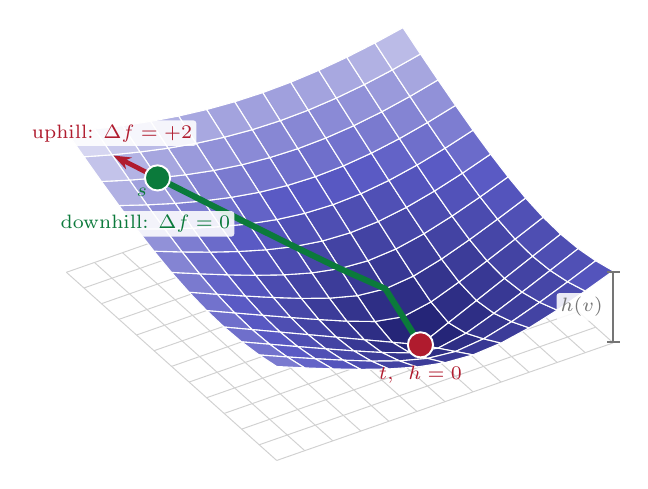
\begin{tikzpicture}
  \begin{axis}[land3d, land view={-32}{34}{0.42}]
    \floorA
    \addplot3[tilesurf, colormap name=hblue, samples=13, samples y=13,
              domain=0:12, y domain=0:12]
      {\kA*veclen(x-\gAx, y-\gAy)};
    \draw[neutralg, line width=0.6pt, {Bar[width=1.6mm]}-{Bar[width=1.6mm]}]
      (12,0,0) -- \liftA{12}{0}
      node[tagbox, text=neutralg, midway, left=2pt] {$h(v)$};
    \draw[edgpath, line cap=round, line join=round]
      \liftA{2}{10} -- \liftA{3}{9} -- \liftA{4}{8} -- \liftA{5}{7}
      -- \liftA{6}{6} -- \liftA{7}{5} -- \liftA{7}{4} -- \liftA{7}{3};
    \draw[move3d,cbRed] \liftA{2}{10} -- \liftA{1}{11};
    \node[tagbox, text=cbRed, above=3pt] at \liftA{1}{11} {uphill: $\Delta f=+2$};
    \node[tagbox, text=cbGreen, left=5pt] at \liftA{4}{8} {downhill: $\Delta f=0$};
    \node[sball] at \liftA{2}{10} {};
    \node[tag, text=gstart, below left=3pt] at \liftA{2}{10} {$s$};
    \node[gball] at \liftA{7}{3} {};
    \node[tag, text=ggoal, below=6pt] at \liftA{7}{3} {$t$, \ $h=0$};
  \end{axis}
\end{tikzpicture}

    \caption{A $12 \times 12$ map lifted by the Euclidean heuristic. The path
      from $s$ runs downhill to $t$.}\label{fig:landscape-a}
  \end{subfigure}\hfill
  \begin{subfigure}[b]{0.46\textwidth}\centering
    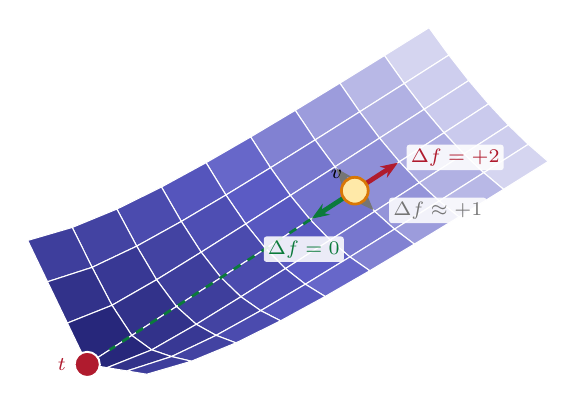
\begin{tikzpicture}
  \begin{axis}[land3d, land view={-24}{30}{0.62}]
    \addplot3[tilesurf, colormap name=hblue, samples=10, samples y=7,
              domain=0:9, y domain=-3:3] {\kB*veclen(x, y)};
    \node[gball] at \liftB{0}{0} {};
    \node[tag, text=ggoal, left=6pt] at \liftB{0}{0} {$t$};
    \draw[cbGreen, dashed, line width=1pt] \liftB{5}{0} -- \liftB{0.5}{0};
    \draw[move3d,cbGreen]  \liftB{6}{0} -- \liftB{5}{0};
    \draw[move3d,cbRed]    \liftB{6}{0} -- \liftB{7}{0};
    \draw[move3d,neutralg] \liftB{6}{0} -- \liftB{6}{1};
    \draw[move3d,neutralg] \liftB{6}{0} -- \liftB{6}{-1};
    \node[vball] at \liftB{6}{0} {};
    \node[tag, above left=4pt] at \liftB{6}{0} {$v$};
    \node[tagbox, text=cbGreen, anchor=north] at \liftB{4.7}{-0.35} {$\Delta f = 0$};
    \node[tagbox, text=cbRed, anchor=west] at \liftB{7.15}{0} {$\Delta f = +2$};
    \node[tagbox, text=neutralg, anchor=west] at \liftB{6.2}{-1.25} {$\Delta f \approx +1$};
  \end{axis}
\end{tikzpicture}

    \caption{Four unit moves out of a vertex $v$ at distance 6 from
      $t$.}\label{fig:landscape-b}
  \end{subfigure}
  \caption{The heuristic as a landscape.}\label{fig:landscape}
\end{figure}

\begin{table}[htbp]
  \centering
  \caption{Change of the key for a unit move out of a vertex at distance 6 from
    the destination, with the Euclidean heuristic.}\label{tab:slope}
  \begin{tabular}{@{}lccc@{}}
    \toprule
    Move & $\Delta g$ & $\Delta h$ & $\Delta f$\\
    \midrule
    toward the destination    & $+1$ & $-1$ & \textcolor{algastar}{$0$}\\
    away from the destination & $+1$ & $+1$ & \textcolor{cbRed}{$+2$}\\
    sideways           & $+1$ & $\sqrt{37} - 6 \approx +0.08$ & $\approx +1.08$\\
    \bottomrule
  \end{tabular}
\end{table}

A move toward the destination leaves the key unchanged, while a move away raises
it by 2. Such moves are not forbidden, only postponed, so A* expands vertices in
the direction of the destination first.

\subsection{Misleading heuristics}\label{sec:bad-h}

Table~\ref{tab:bad-h} lists three ways in which a heuristic can mislead A*.
Only an overestimating heuristic can cost the shortest path; the other two only
waste work.

\begin{table}[htbp]
  \centering
  \caption{Three ways in which a heuristic can mislead A*.}\label{tab:bad-h}
  \renewcommand{\arraystretch}{1.25}%
  \begin{tabular}{@{}P{2.6cm}P{3.4cm}P{2.1cm}P{5.6cm}@{}}
    \toprule
    Kind & Property & Shortest path & Effect\\
    \midrule
    \textcolor{cbRed}{Overestimating} & not admissible & not guaranteed
      & A* behaves like greedy best-first search; on the running example the
        returned cost rises from 8 to 10 (Section~\ref{sec:overestimate})\\
    Uninformative & admissible, nearly constant & guaranteed
      & $h(v) = 1$ for every $v \neq t$ (admissible if every edge costs at
        least 1) adds the same constant to almost every key, so A* expands
        almost the same vertices as Dijkstra's algorithm\\
    \textcolor{alggreedy}{Blind to obstacles} & admissible, ignores walls
      & guaranteed & A* expands dead ends that appear close to the destination, such
        as the inside of the U-shaped wall of Section~\ref{sec:grid}\\
    \bottomrule
  \end{tabular}
\end{table}

\subsubsection{An overestimating heuristic}\label{sec:overestimate}

We place the cities of the running example on a grid at $\cty{D} = (0,4)$, $\cty{N} = (4,6)$,
$\cty{B} = (8,4)$, $\cty{H} = (12,6)$, $\cty{S} = (16,4)$, $\cty{G} = (2,1)$,
$\cty{K} = (8,8)$ and $\cty{C} = (13,1)$ (Figure~\ref{fig:story-m}), and use the Manhattan distance $h_{M}$ to \cty{S} as the heuristic. The grid
units are unrelated to the edge weights, and $h_{M}$ overestimates in six of the
eight cities (Table~\ref{tab:story-hm}).

\begin{table}[htbp]
  \centering
  \caption{Two heuristics for the running example and the true remaining cost.
    Red values overestimate.}\label{tab:story-hm}
  \begin{tabular}{@{}lcccccccc@{}}
    \toprule
    City & \cty{D} & \cty{G} & \cty{N} & \cty{K} & \cty{B} & \cty{C} & \cty{H} & \cty{S}\\
    \midrule
    Heuristic $h$ (Table~\ref{tab:story-h}) & 7 & 8 & 5 & 4 & 4 & 7 & 2 & 0\\
    Manhattan distance $h_{M}$ & \textcolor{cbRed}{16} & \textcolor{cbRed}{17}
      & \textcolor{cbRed}{14} & \textcolor{cbRed}{12} & \textcolor{cbRed}{8}
      & 6 & \textcolor{cbRed}{6} & 0\\
    True cost $h^{*}$     & 8 & 9 & 6 & 7 & 5 & 8 & 3 & 0\\
    \bottomrule
  \end{tabular}
\end{table}

With $h_{M}$, A* returns $(\cty{D}, \cty{B}, \cty{H}, \cty{S})$ of cost 10
(Table~\ref{tab:trace-m}). The cause is $h_{M}(\cty{N}) = 14$, more than twice
$h^{*}(\cty{N}) = 6$: after step 1, \cty{N} has key 16 and \cty{B} key 13, so
the search reaches \cty{S} with $g = 10$ before expanding \cty{N}. With
$h(\cty{N}) = 5$, the key of \cty{N} would be $7 < 10$. When $h$ dominates $g$,
A* behaves like greedy best-first search and returns the same path.

\begin{table}[htbp]
  \centering
  \caption{A* on the running example with the Manhattan distance $h_{M}$, which
    overestimates.}\label{tab:trace-m}
  \small
  \begin{tabular}{@{}c>{\raggedright}P{4.8cm}cc>{\raggedright\arraybackslash}P{3.4cm}@{}}
    \toprule
    Step & $Q$ before extraction (vertex: key) & Extracted & $g + h_{M} = f$
      & Updates\\
    \midrule
    \inputrows{figures/trace_manhattan.tex}
    \bottomrule
  \end{tabular}
\end{table}

\begin{figure}[htbp]
  \centering
  \resizebox{0.62\textwidth}{!}{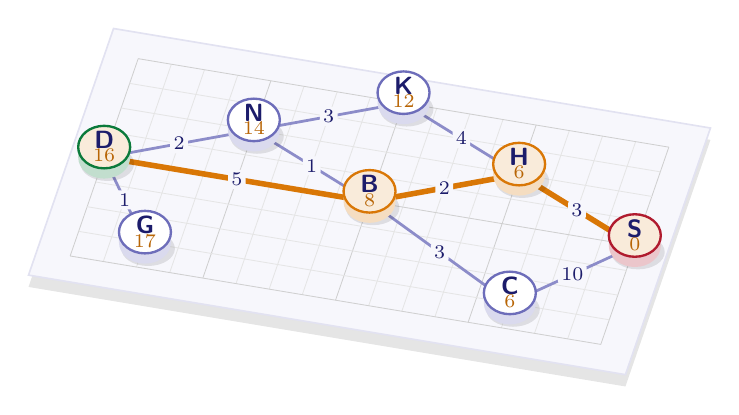
\begin{tikzpicture}[x=1cm, y=1cm]
  \fill[black!10] (-0.529,-0.393) -- (7.052,-1.657) -- (8.132,1.475) -- (0.551,2.739) -- cycle;
  \draw[draw=rblue!14, fill=rbluelt!35, line width=0.6pt] (-0.529,-0.243) -- (7.052,-1.507) -- (8.132,1.625) -- (0.551,2.889) -- cycle;
  \draw[black!19, line width=0.3pt] (0.000,0.000) -- (0.864,2.506);
  \draw[black!10, line width=0.3pt] (0.421,-0.070) -- (1.285,2.435);
  \draw[black!10, line width=0.3pt] (0.842,-0.140) -- (1.706,2.365);
  \draw[black!10, line width=0.3pt] (1.264,-0.211) -- (2.128,2.295);
  \draw[black!19, line width=0.3pt] (1.685,-0.281) -- (2.549,2.225);
  \draw[black!10, line width=0.3pt] (2.106,-0.351) -- (2.970,2.155);
  \draw[black!10, line width=0.3pt] (2.527,-0.421) -- (3.391,2.084);
  \draw[black!10, line width=0.3pt] (2.948,-0.491) -- (3.812,2.014);
  \draw[black!19, line width=0.3pt] (3.370,-0.562) -- (4.234,1.944);
  \draw[black!10, line width=0.3pt] (3.791,-0.632) -- (4.655,1.874);
  \draw[black!10, line width=0.3pt] (4.212,-0.702) -- (5.076,1.804);
  \draw[black!10, line width=0.3pt] (4.633,-0.772) -- (5.497,1.733);
  \draw[black!19, line width=0.3pt] (5.054,-0.842) -- (5.918,1.663);
  \draw[black!10, line width=0.3pt] (5.476,-0.913) -- (6.340,1.593);
  \draw[black!10, line width=0.3pt] (5.897,-0.983) -- (6.761,1.523);
  \draw[black!10, line width=0.3pt] (6.318,-1.053) -- (7.182,1.453);
  \draw[black!19, line width=0.3pt] (6.739,-1.123) -- (7.603,1.382);
  \draw[black!19, line width=0.3pt] (0.000,0.000) -- (6.739,-1.123);
  \draw[black!10, line width=0.3pt] (0.108,0.313) -- (6.847,-0.810);
  \draw[black!10, line width=0.3pt] (0.216,0.626) -- (6.955,-0.497);
  \draw[black!10, line width=0.3pt] (0.324,0.940) -- (7.063,-0.184);
  \draw[black!19, line width=0.3pt] (0.432,1.253) -- (7.171,0.130);
  \draw[black!10, line width=0.3pt] (0.540,1.566) -- (7.279,0.443);
  \draw[black!10, line width=0.3pt] (0.648,1.879) -- (7.387,0.756);
  \draw[black!10, line width=0.3pt] (0.756,2.192) -- (7.495,1.069);
  \draw[black!19, line width=0.3pt] (0.864,2.506) -- (7.603,1.382);
  \coordinate (D) at (0.432,1.253);
  \coordinate (N) at (2.333,1.598);
  \coordinate (B) at (3.802,0.691);
  \coordinate (H) at (5.702,1.037);
  \coordinate (S) at (7.171,0.130);
  \coordinate (G) at (0.950,0.173);
  \coordinate (K) at (4.234,1.944);
  \coordinate (C) at (5.584,-0.599);
  \draw[draw=rblue!55, line width=1pt] (D) -- (N);
  \draw[draw=alggreedy, line width=2pt] (D) -- (B);
  \draw[draw=rblue!55, line width=1pt] (N) -- (B);
  \draw[draw=alggreedy, line width=2pt] (B) -- (H);
  \draw[draw=alggreedy, line width=2pt] (H) -- (S);
  \draw[draw=rblue!55, line width=1pt] (D) -- (G);
  \draw[draw=rblue!55, line width=1pt] (N) -- (K);
  \draw[draw=rblue!55, line width=1pt] (K) -- (H);
  \draw[draw=rblue!55, line width=1pt] (B) -- (C);
  \draw[draw=rblue!55, line width=1pt] (C) -- (S);
  \node[isoweight] at ($(D)!0.5!(N)$) {2};
  \node[isoweight] at ($(D)!0.5!(B)$) {5};
  \node[isoweight] at ($(N)!0.5!(B)$) {1};
  \node[isoweight] at ($(B)!0.5!(H)$) {2};
  \node[isoweight] at ($(H)!0.5!(S)$) {3};
  \node[isoweight] at ($(D)!0.5!(G)$) {1};
  \node[isoweight] at ($(N)!0.5!(K)$) {3};
  \node[isoweight] at ($(K)!0.5!(H)$) {4};
  \node[isoweight] at ($(B)!0.5!(C)$) {3};
  \node[isoweight] at ($(C)!0.5!(S)$) {10};
  \isodisc{D}{alggreedy!15}{algastar}{D}{16}
  \isodisc{N}{white}{rblue!70}{N}{14}
  \isodisc{B}{alggreedy!15}{alggreedy}{B}{8}
  \isodisc{H}{alggreedy!15}{alggreedy}{H}{6}
  \isodisc{S}{alggreedy!15}{cbRed}{S}{0}
  \isodisc{G}{white}{rblue!70}{G}{17}
  \isodisc{K}{white}{rblue!70}{K}{12}
  \isodisc{C}{white}{rblue!70}{C}{6}
\end{tikzpicture}
}
  \caption{The running example on its grid, with the Manhattan distance $h_{M}$
    in each disc. A* now returns the orange path, which is not the shortest
    one.}\label{fig:story-m}
\end{figure}

Figure~\ref{fig:estimates} compares three estimates for \cty{N}; only the one
above the true cost leads A* astray.

\begin{figure}[htbp]
  \centering
  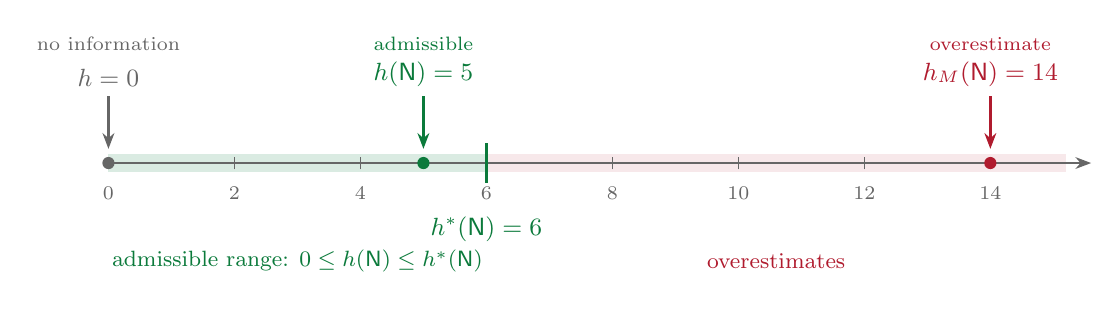
\begin{tikzpicture}[x=0.8cm, y=1cm]
    \fill[algastar!15] (0,-0.12) rectangle (6,0.12);
    \fill[cbRed!10] (6,-0.12) rectangle (15.2,0.12);
    \draw[inkgray, line width=0.6pt, -{Stealth[length=2mm]}] (0,0) -- (15.6,0);
    \foreach \x in {0,2,...,14}
      {\draw[inkgray] (\x,-0.08) -- (\x,0.08);
       \node[font=\scriptsize, text=inkgray, below=3pt] at (\x,-0.08) {\x};}
    \draw[algastar, line width=1pt] (6,-0.25) -- (6,0.25);
    \node[font=\small, text=algastar, below=16pt] at (6,0) {$h^{*}(\cty{N}) = 6$};
    \foreach \x/\c/\lab/\note in {0/inkgray/{$h = 0$}/{no information},
                                  5/algastar/{$h(\cty{N}) = 5$}/{admissible},
                                  14/cbRed/{$h_M(\cty{N}) = 14$}/{overestimate}}
      {\draw[\c, line width=0.9pt, -{Stealth[length=2mm]}] (\x,0.85) -- (\x,0.18);
       \fill[\c] (\x,0) circle (2.2pt);
       \node[font=\small, text=\c, above] at (\x,0.85) {\lab};
       \node[font=\scriptsize, text=\c, above=13pt] at (\x,0.85) {\note};}
    \node[font=\footnotesize, text=algastar] at (3,-1.25) {admissible range:
      $0 \le h(\cty{N}) \le h^{*}(\cty{N})$};
    \node[font=\footnotesize, text=cbRed] at (10.6,-1.25) {overestimates};
  \end{tikzpicture}
  \caption{Three estimates of the remaining cost from \cty{N}, compared with the
    true cost $h^{*}(\cty{N}) = 6$.}\label{fig:estimates}
\end{figure}

\section{Correctness}\label{sec:correctness}

When is the path returned by A* a cheapest one? Table~\ref{tab:guarantees}
summarizes the answer, which depends on the heuristic. Throughout this section,
$G = (V,E,w)$ is finite with nonnegative weights, $t$ is reachable from $s$, and
$C^{*} = \delta(s,t)$; the key of a vertex $u$ in $Q$ is $f(u) = g(u) + h(u)$.

\begin{table}[htbp]
  \centering
  \caption{What A* guarantees for each kind of heuristic.}\label{tab:guarantees}
  \renewcommand{\arraystretch}{1.25}%
  \begin{tabular}{@{}P{3.2cm}P{4.1cm}P{3.4cm}P{2.8cm}@{}}
    \toprule
    Heuristic & Algorithm~\ref{alg:astar} (closed set) & A* with reopening
      & Result\\
    \midrule
    consistent & \textcolor{algastar}{shortest path}, each vertex expanded
      at most once & \textcolor{algastar}{shortest path}
      & Theorem~\ref{thm:consistent}\\
    admissible, not consistent & \textcolor{cbRed}{may fail}
      (Example~\ref{ex:inconsistent}) & \textcolor{algastar}{shortest path}
      & Theorem~\ref{thm:admissible}\\
    not admissible & \textcolor{cbRed}{may fail}
      (Section~\ref{sec:overestimate}) & \textcolor{cbRed}{may fail} & none\\
    $h(v) = 0$ for all $v$ (Dijkstra's algorithm)
      & \textcolor{algastar}{shortest path} & \textcolor{algastar}{shortest path}
      & Corollary~\ref{cor:dijkstra}\\
    \bottomrule
  \end{tabular}
\end{table}

\subsection{Two facts about the cost so far}\label{sec:invariant}

The values $g(v)$ only go down and never drop below the true distance from the
source. The same proof applies to A* with reopening
(Section~\ref{sec:admissible-proof}). A \emph{walk} is like a path but may
visit a vertex more than once.

\begin{lemma}\label{lem:invariant}
During the execution of Algorithm~\ref{alg:astar}, the value $g(v)$ of a vertex
$v$ never increases. Whenever $g(v)$ is finite, it is the cost of some walk from
$s$ to $v$, and consequently $g(v) \ge \delta(s,v)$.
\end{lemma}

\begin{proof}
The algorithm changes $g(v)$ only by the assignment $g(v) \gets g(u) + w(u,v)$,
and only when the new value is smaller, so $g(v)$ never increases. We prove the
second claim by induction on the number of assignments. Initially only $g(s)$ is
finite, and $g(s) = 0$ is the cost of the walk $(s)$. An assignment sets
$g(v) = g(u) + w(u,v)$, where, by the induction hypothesis, $g(u)$ is the cost
of a walk from $s$ to $u$. Appending $v$ to this walk gives a walk from $s$ to
$v$ of cost $g(v)$. Finally, removing the repeated parts of a walk yields a path
between the same vertices, and the path costs no more than the walk because
every weight is nonnegative. Hence $g(v) \ge \delta(s,v)$.
\end{proof}

\subsection{Consistent heuristics}\label{sec:consistent-proof}

With a consistent heuristic, the estimated total cost never decreases along a
path.

\begin{lemma}\label{lem:pathmono}
Let $h$ be a consistent heuristic and let $P = (v_0, v_1, \dots, v_k)$ be a
path. For $0 \le i \le k$, let $f_P(v_i) = c(v_0, \dots, v_i) + h(v_i)$, where
$c(v_0, \dots, v_i)$ is the cost of the first $i$ edges of $P$. Then
$f_P(v_0) \le f_P(v_1) \le \dots \le f_P(v_k)$.
\end{lemma}

\begin{proof}
For $1 \le i \le k$, Inequality~\eqref{eq:consistent} applied to the edge
$(v_{i-1}, v_i)$ gives
\begin{equation}\label{eq:fstep}
  f_P(v_i) = f_P(v_{i-1}) + w(v_{i-1}, v_i) + h(v_i) - h(v_{i-1})
           \ge f_P(v_{i-1}). \qedhere
\end{equation}
\end{proof}

Consequently, the extracted keys never decrease.

\begin{lemma}\label{lem:monotone}
Let $h$ be a consistent heuristic. Then Algorithm~\ref{alg:astar} extracts
vertices from $Q$ in nondecreasing order of their keys.
\end{lemma}

\begin{proof}
Suppose that the algorithm extracts a vertex $u$ with key $f(u)$. At that moment
every key in $Q$ is at least $f(u)$, because \textsc{Extract-Min} returns a
smallest key. While $u$ is expanded, a key is inserted or decreased only to a
value $g(u) + w(u,v) + h(v)$ for a neighbor $v$ of $u$, and by
Inequality~\eqref{eq:consistent} this value is at least $g(u) + h(u) = f(u)$.
Hence every key in $Q$ is still at least $f(u)$ at the next extraction, and the
next extracted key is at least $f(u)$.
\end{proof}

The main lemma states that a vertex leaves $Q$ only when its value $g$ is exact
(Figure~\ref{fig:proof-idea}).

\begin{figure}[htbp]
  \centering
  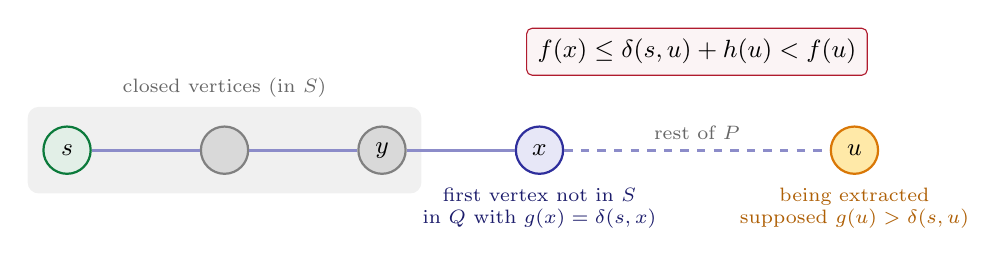
\begin{tikzpicture}[x=1cm, y=1cm]
  \fill[gray!12, rounded corners=4pt] (-0.5,-0.55) rectangle (4.5,0.55);
  \node[font=\scriptsize, text=inkgray, anchor=south] at (2,0.55) {closed vertices (in $S$)};
  \node[storystart] (s) at (0,0) {$s$};
  \node[storynode, fill=gray!30, draw=gray] (a) at (2,0) {};
  \node[storynode, fill=gray!30, draw=gray] (y) at (4,0) {$y$};
  \node[storynode, fill=rbluelt] (x) at (6,0) {$x$};
  \node[storynode, fill=hlyellow, draw=alggreedy] (u) at (10,0) {$u$};
  \draw[storyedge, line width=1.2pt] (s) -- (a) -- (y) -- (x);
  \draw[storyedge, line width=1.2pt, dashed] (x) -- node[above, font=\scriptsize,
    text=inkgray] {rest of $P$} (u);
  \node[font=\scriptsize, text=rbluedk, below=10pt, align=center] at (x)
    {first vertex not in $S$\\in $Q$ with $g(x) = \delta(s,x)$};
  \node[font=\scriptsize, text=alggreedy!80!black, below=10pt, align=center] at (u)
    {being extracted\\supposed $g(u) > \delta(s,u)$};
  \node[draw=cbRed, fill=cbRed!5, font=\small, rounded corners=2pt, inner sep=4pt]
    at (8,1.25) {$f(x) \le \delta(s,u) + h(u) < f(u)$};
\end{tikzpicture}

  \caption{The idea behind Lemma~\ref{lem:exact}. On a shortest path $P$ from
    $s$ to $u$, the first vertex $x$ that is not closed is in $Q$ with an exact
    value $g(x)$, and its key is smaller than the key of $u$.}\label{fig:proof-idea}
\end{figure}

\begin{lemma}\label{lem:exact}
Let $h$ be a consistent heuristic. Whenever Algorithm~\ref{alg:astar} extracts a
vertex $u$ from $Q$, we have $g(u) = \delta(s,u)$.
\end{lemma}

\begin{proof}
Suppose the contrary, and let $u$ be the first extracted vertex with
$g(u) \ne \delta(s,u)$; by Lemma~\ref{lem:invariant}, $g(u) > \delta(s,u)$. The
first iteration extracts $s$ with $g(s) = 0 = \delta(s,s)$, so $u \neq s$. The
value $g(u)$ is finite, so $u$ is reachable from $s$; let $P$ be a shortest path
from $s$ to $u$. Just before $u$ is extracted, $s$ is in $S$ and $u$ is not. Let
$x$ be the first vertex of $P$ that is not in $S$, and let $y$ be the vertex
that precedes $x$ on $P$; then $y$ is in $S$.

The vertex $y$ was extracted before $u$, so $g(y) = \delta(s,y)$ by the choice
of $u$. When $y$ was expanded, the vertex $x$ was not in $S$, because $S$ only
grows, and the relaxation of the edge $(y,x)$ ensured that
$g(x) \le \delta(s,y) + w(y,x) = \delta(s,x)$; the equality holds because the
part of $P$ from $s$ to $x$ is a shortest path. By Lemma~\ref{lem:invariant},
$g(x)$ has not increased since and is at least $\delta(s,x)$, so
$g(x) = \delta(s,x)$. A vertex with a finite value $g$ that is not in $S$ is in
$Q$, so $x$ is in $Q$. Moreover $x \neq u$, because $g(u) > \delta(s,u)$.

Lemma~\ref{lem:pathmono}, applied to $P$, compares the keys of $x$ and $u$. The
costs of the parts of $P$ that end at $x$ and at $u$ are $\delta(s,x)$ and
$\delta(s,u)$, so
\begin{equation}\label{eq:xbeforeu}
  f(x) = \delta(s,x) + h(x) \le \delta(s,u) + h(u) < g(u) + h(u) = f(u).
\end{equation}
The vertex $x$ is in $Q$ with a smaller key than $u$, which contradicts the
choice of $u$ by \textsc{Extract-Min}.
\end{proof}

We can now prove the main result.

\begin{theorem}[Optimality of A* with a consistent heuristic]\label{thm:consistent}
Let $G$ be a finite graph with nonnegative edge weights, let $s$ and $t$ be
vertices of $G$ such that $t$ is reachable from $s$, and let $h$ be a
consistent heuristic. Then Algorithm~\ref{alg:astar} expands every vertex at
most once and returns a path from $s$ to $t$ of cost $\delta(s,t)$.
\end{theorem}

\begin{proof}
A vertex enters $S$ when it is extracted and never leaves $S$, and the loop over
the edges never inserts a vertex of $S$ into $Q$. Hence every vertex is extracted
at most once, and the algorithm stops after at most $|V|$ iterations.

The algorithm does not return failure. Suppose, to the contrary, that $Q$
becomes empty before $t$ is extracted. Consider a path from $s$ to $t$; its
first vertex $s$ is in $S$ and its last vertex $t$ is not. Let $x$ be the first
vertex of the path that is not in $S$. The vertex that precedes $x$ on the path
is in $S$, and its expansion gave $x$ a finite value $g(x)$ and inserted $x$
into $Q$. The vertex $x$ can leave $Q$ only by being extracted, after which it
would be in $S$ or the algorithm would have returned. Both cases contradict the
assumptions, so the algorithm extracts $t$, and $g(t) = \delta(s,t)$ at that
moment by Lemma~\ref{lem:exact}.

It remains to show that the returned path has cost $g(t)$. Let $v \neq s$ be a
vertex on the path and let $p = \pi(v)$. The last change of $g(v)$ and $\pi(v)$
happened during the expansion of $p$ and set $g(v) = g(p) + w(p,v)$. The value
$g(p)$ did not change afterwards, because $p$ was in $S$. The vertex $p$ was
extracted before $v$, so following the predecessors from $t$ visits vertices in
strictly decreasing order of extraction and therefore reaches $s$. Adding the
equalities $g(v) - g(\pi(v)) = w(\pi(v), v)$ along the path shows that its cost
is $g(t) - g(s) = \delta(s,t)$.
\end{proof}

Dijkstra's algorithm is the special case of the zero heuristic.

\begin{corollary}\label{cor:dijkstra}
Let $G$ be a finite graph with nonnegative edge weights, and let $s$ and $t$ be
vertices of $G$ such that $t$ is reachable from $s$. Then
Algorithm~\ref{alg:dijkstra} returns a shortest path from $s$ to $t$.
\end{corollary}

\begin{proof}
The zero heuristic, $h(v) = 0$ for every vertex $v$, is consistent, because
$0 \le w(u,v) + 0$ for every edge $(u,v)$. With this heuristic the key $g + h$
equals $g$, so Algorithm~\ref{alg:astar} is Algorithm~\ref{alg:dijkstra}. The
claim follows from Theorem~\ref{thm:consistent}.
\end{proof}

\subsection{Admissible heuristics}\label{sec:admissible-proof}

Admissibility alone does not make Algorithm~\ref{alg:astar} correct.

\begin{example}\label{ex:inconsistent}
Consider the graph of Figure~\ref{fig:counterexample} with source $s$ and destination
$t$. The shortest path is $(s, a, c, t)$, of cost 5. The true remaining costs
are $h^{*}(s) = 5$, $h^{*}(a) = 4$, $h^{*}(b) = 5$ and $h^{*}(c) = 3$, so the
heuristic shown in the figure is admissible. It is not consistent, because
$h(a) = 4 > w(a,c) + h(c) = 2$. Table~\ref{tab:counterexample} traces
Algorithm~\ref{alg:astar} on this graph. In step 4 the edge $(a,c)$ offers $c$
the smaller value $1 + 1 = 2$, but $c$ is already closed, so the algorithm skips
the edge and returns $(s, b, c, t)$, of cost 6.
\end{example}

\begin{figure}[htbp]
  \centering
  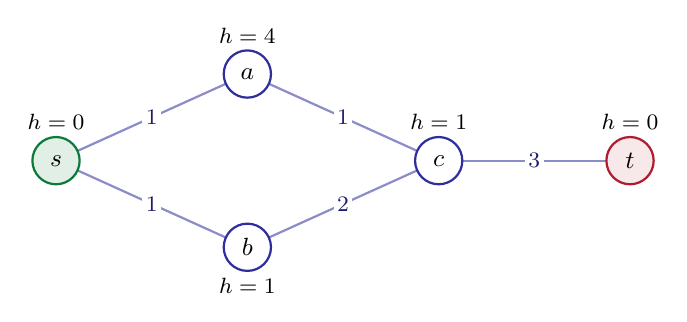
\begin{tikzpicture}[x=1.35cm, y=1.1cm]
  \coordinate (s) at (0,0);
  \coordinate (a) at (1.8,1.0);
  \coordinate (b) at (1.8,-1.0);
  \coordinate (c) at (3.6,0);
  \coordinate (t) at (5.4,0);
  \draw[storyedge] (s) -- node[storyweight] {1} (a);
  \draw[storyedge] (a) -- node[storyweight] {1} (c);
  \draw[storyedge] (s) -- node[storyweight] {1} (b);
  \draw[storyedge] (b) -- node[storyweight] {2} (c);
  \draw[storyedge] (c) -- node[storyweight] {3} (t);
  \node[storystart] at (s) {$s$};
  \node[storyh, above=11pt] at (s) {$h=0$};
  \node[storynode] at (a) {$a$};
  \node[storyh, above=11pt] at (a) {$h=4$};
  \node[storynode] at (b) {$b$};
  \node[storyh, below=11pt] at (b) {$h=1$};
  \node[storynode] at (c) {$c$};
  \node[storyh, above=11pt] at (c) {$h=1$};
  \node[storygoal] at (t) {$t$};
  \node[storyh, above=11pt] at (t) {$h=0$};
\end{tikzpicture}

  \caption{An admissible heuristic that is not consistent. Edge weights are on
    the edges, and heuristic values are beside the vertices.}\label{fig:counterexample}
\end{figure}

\begin{table}[htbp]
  \centering
  \caption{Algorithm~\ref{alg:astar} on the graph of
    Figure~\ref{fig:counterexample}.}\label{tab:counterexample}
  \begin{tabular}{@{}clll@{}}
    \toprule
    Step & Extracted (key) & Updates & State of $c$\\
    \midrule
    1 & $s$ (0) & $g(a) = 1$, key 5; \ $g(b) = 1$, key 2 & not reached\\
    2 & $b$ (2) & $g(c) = 3$, key 4 & in $Q$, $g(c) = 3$\\
    3 & $c$ (4) & $g(t) = 6$, key 6 & closed, $g(c) = 3$\\
    4 & $a$ (5) & \textcolor{cbRed}{edge $(a,c)$ skipped, $c$ is closed}
      & closed, $g(c) = 3$\\
    5 & $t$ (6) & returns $(s,b,c,t)$, cost \textcolor{cbRed}{6} & \\
    \bottomrule
  \end{tabular}
\end{table}

Here $c$ was closed before $g(c)$ was exact, and the closed set blocked the
correction. \emph{A* with reopening} removes the condition ``$v$ is not in $S$''
from Algorithm~\ref{alg:astar} and moves every vertex whose $g$ decreases back
from $S$ into $Q$. On Example~\ref{ex:inconsistent} it reopens $c$ with key 3 and
returns $(s,a,c,t)$ of cost 5.

\begin{theorem}[Optimality of A* with an admissible heuristic]\label{thm:admissible}
Let $G$ be a finite graph in which every edge weight is positive, let $s$ and $t$
be vertices of $G$ such that $t$ is reachable from $s$, and let $h$ be an
admissible heuristic. Then A* with reopening terminates and returns a path from
$s$ to $t$ of cost $\delta(s,t)$.
\end{theorem}

\begin{proof}
We first prove termination. Let $w_{\min} > 0$ be the smallest edge weight, let
$v$ be a vertex, and let $g_{0}$ be the first finite value of $g(v)$. By
Lemma~\ref{lem:invariant}, every later value of $g(v)$ is the cost of a walk
from $s$ to $v$ of cost at most $g_{0}$. Such a walk has at most
$g_{0} / w_{\min}$ edges, so there are finitely many such walks, and $g(v)$
takes finitely many values. After an extraction, the vertex $v$ returns to $Q$
only if $g(v)$ decreases, so $v$ is extracted at most once for each value of
$g(v)$. Hence the number of iterations is finite.

Let $P^{*} = (s = v_0, v_1, \dots, v_k = t)$ be a shortest path from $s$ to
$t$. We show that before every extraction that precedes the extraction of $t$,
some vertex $v_j$ of $P^{*}$ is in $Q$ with $g(v_j) = \delta(s,v_j)$. In
particular $Q$ is not empty, so the algorithm does not return failure. Let $j$
be the largest index with $g(v_j) = \delta(s,v_j)$; it exists because
$g(s) = 0$. Suppose that $v_j$ is not in $Q$. Since $g(v_j)$ is finite, $v_j$
has been reached, so it is in $S$; in particular $v_j \neq t$, because the
extraction of $t$ ends the search. The value $g(v_j)$ did not decrease after the
last expansion of $v_j$, because a decrease would have reopened $v_j$. Hence
$g(v_j) = \delta(s,v_j)$ during that expansion, which relaxed the edge
$(v_j, v_{j+1})$ and set
$g(v_{j+1}) \le \delta(s,v_j) + w(v_j,v_{j+1}) = \delta(s,v_{j+1})$. By
Lemma~\ref{lem:invariant}, $g(v_{j+1}) = \delta(s,v_{j+1})$ from then on, which
contradicts the choice of $j$. So $v_j$ is in $Q$.

When $t$ is extracted, its key is $g(t) + h(t) = g(t)$, because admissibility
gives $0 \le h(t) \le h^{*}(t) = 0$. Just before this extraction, the vertex
$v_j$ found above is in $Q$ with key
\begin{equation}\label{eq:admbound}
  \delta(s,v_j) + h(v_j) \le \delta(s,v_j) + h^{*}(v_j) = C^{*},
\end{equation}
where the equality holds because $v_j$ lies on a shortest path from $s$ to $t$.
\textsc{Extract-Min} chose $t$, so $g(t) \le C^{*}$. Together with
$g(t) \ge C^{*}$ from Lemma~\ref{lem:invariant}, this gives $g(t) = C^{*}$.

Finally, consider the returned path. For every vertex $v \neq s$ on it, the last
change of $g(v)$ and $\pi(v)$ set $g(v) = g(\pi(v)) + w(\pi(v), v)$, and
$g(\pi(v))$ can only have decreased since. Hence
$g(\pi(v)) + w(\pi(v), v) \le g(v)$. Every weight is positive, so $g$ strictly
decreases along the predecessors; the path therefore visits no vertex twice and
ends at $s$. Adding the inequalities along the path shows that its cost is at
most $g(t) - g(s) = C^{*}$. No path costs less than $C^{*}$, so the cost of the
returned path is exactly $C^{*}$.
\end{proof}

Theorem~\ref{thm:admissible} is the original result of Hart, Nilsson and
Raphael~\cite{hart1968formal}; Theorem~\ref{thm:consistent} covers the usual
implementation~\cite{russell2020aima}, in which each vertex is expanded at most
once. With an inconsistent heuristic a vertex may be expanded many times
(Section~\ref{sec:complexity}).

\section{Time and space complexity}\label{sec:complexity}

We analyze Algorithm~\ref{alg:astar} with a consistent heuristic, where $|V|$
and $|E|$ are the numbers of vertices and edges. We assume that $Q$ is a binary
heap, in which each queue operation takes $O(\log |V|)$ time, and that $h(v)$ is
computed in constant time, as for the distance heuristics.

\subsection{Time}\label{sec:time}

By Theorem~\ref{thm:consistent}, every vertex is extracted at most once, so
every edge is examined at most twice (Table~\ref{tab:time}).

\begin{table}[htbp]
  \centering
  \caption{Running time of Algorithm~\ref{alg:astar} with a binary
    heap.}\label{tab:time}
  \renewcommand{\arraystretch}{1.25}%
  \begin{tabular}{@{}P{4.4cm}P{4.6cm}P{2.2cm}P{2.6cm}@{}}
    \toprule
    Operation & Number of executions & Cost of each & Total\\
    \midrule
    initialization of $g$ and $\pi$ & once per vertex & $O(1)$ & $O(|V|)$\\
    \textsc{Extract-Min} & at most once per vertex & $O(\log|V|)$
      & $O(|V|\log|V|)$\\
    examination of an edge & at most twice per edge & $O(1)$ & $O(|E|)$\\
    \textsc{Insert-or-Decrease-Key} & at most once per examination of an edge
      & $O(\log|V|)$ & $O(|E|\log|V|)$\\
    \bottomrule
  \end{tabular}
\end{table}

Summing the totals gives the running time
\begin{equation}\label{eq:time}
  O(|V|) + O(|V| \log |V|) + O(|E|) + O(|E| \log |V|)
  = O\big((|V| + |E|) \log |V|\big).
\end{equation}

This is also the bound for Dijkstra's algorithm, and a Fibonacci heap reduces
both to $O(|E| + |V| \log |V|)$~\cite{cormen2022clrs}. In the worst case A* is
no faster than Dijkstra's algorithm, since the zero heuristic is consistent; its
advantage lies in the number of vertices expanded
(Section~\ref{sec:efficiency}).

With an inconsistent heuristic, A* with reopening can expand a vertex many
times; Martelli~\cite{martelli1977} gave graphs on which the number of
expansions grows exponentially.

\subsection{Space}\label{sec:space}

Each item of Table~\ref{tab:space} holds at most one entry per vertex, so the
memory is $O(|V|)$.

\begin{table}[htbp]
  \centering
  \caption{Memory used by Algorithm~\ref{alg:astar}.}\label{tab:space}
  \renewcommand{\arraystretch}{1.25}%
  \begin{tabular}{@{}P{5cm}P{6cm}P{2.4cm}@{}}
    \toprule
    Data & Size & Total\\
    \midrule
    values $g$ and predecessors $\pi$ & one entry per vertex & $O(|V|)$\\
    closed set $S$ & at most every vertex & $O(|V|)$\\
    priority queue $Q$ & at most one entry per vertex, with
      \textsc{Decrease-Key} & $O(|V|)$\\
    reconstructed path & at most $|V|$ vertices & $O(|V|)$\\
    \midrule
    \textbf{Total} & & $O(|V|)$\\
    \bottomrule
  \end{tabular}
\end{table}

Implementations that insert a second queue entry instead of decreasing a key
need $O(|V| + |E|)$ space. On large graphs memory, not time, is usually the
limit, because A* stores every vertex it reaches~\cite{russell2020aima}.

\subsection{Comparison of the three algorithms}\label{sec:complexity-compare}

In greedy best-first search every vertex enters $Q$ once and no key decreases,
which gives the smallest bound in Table~\ref{tab:complexity}. The worst-case
bounds do not separate A* from Dijkstra's algorithm.

\begin{table}[htbp]
  \centering
  \caption{Worst-case complexity of the three algorithms with a binary heap and
    a consistent heuristic.}\label{tab:complexity}
  \renewcommand{\arraystretch}{1.25}%
  \begin{tabular}{@{}P{2.6cm}P{3.6cm}P{3.6cm}P{3.6cm}@{}}
    \toprule
     & \textcolor{algdijkstra}{\textbf{Dijkstra's algorithm}}
     & \textcolor{alggreedy}{\textbf{Greedy best-first search}}
     & \textcolor{algastar}{\textbf{A* search}}\\
    \midrule
    Time  & $O((|V|{+}|E|)\log|V|)$ & $O(|E| + |V|\log|V|)$
      & $O((|V|{+}|E|)\log|V|)$\\[2pt]
    Space & $O(|V|)$ & $O(|V|)$ & $O(|V|)$\\[2pt]
    Shortest path & \textcolor{algastar}{guaranteed}
      & \textcolor{cbRed}{not guaranteed} & \textcolor{algastar}{guaranteed}\\
    \bottomrule
  \end{tabular}
\end{table}

\section{Why A* expands fewer vertices}\label{sec:efficiency}

Although the worst-case bounds coincide, A* expands far fewer vertices than
Dijkstra's algorithm in practice. This section characterizes the vertices it
expands and measures the effect on a grid with an obstacle.

\subsection{The vertices that A* expands}\label{sec:expanded}

\begin{proposition}\label{prop:expanded}
Let $G$ be a finite graph with nonnegative edge weights, let $t$ be reachable
from $s$, and let $h$ be a consistent heuristic. Then Algorithm~\ref{alg:astar}
has the following two properties.
\begin{enumerate}[label=(\alph*)]
  \item Every vertex $u$ that it extracts satisfies
    $\delta(s,u) + h(u) \le C^{*}$.
  \item Every vertex $u$ with $\delta(s,u) + h(u) < C^{*}$ is extracted before
    $t$.
\end{enumerate}
\end{proposition}

\begin{proof}
(a) By Lemma~\ref{lem:exact}, a vertex $u$ is extracted with key
$g(u) + h(u) = \delta(s,u) + h(u)$. The destination is extracted last, with key
$\delta(s,t) + h(t) = C^{*}$, and by Lemma~\ref{lem:monotone} no earlier key is
larger.

(b) Suppose that such a vertex $u$ is not in $S$ when $t$ is extracted. Let $P$
be a shortest path from $s$ to $u$, and let $x$ be the first vertex of $P$ that
is not in $S$. The argument of the proof of Lemma~\ref{lem:exact} shows that $x$
is in $Q$ with $g(x) = \delta(s,x)$, and Lemma~\ref{lem:pathmono} gives
$f(x) \le \delta(s,u) + h(u) < C^{*}$. The key of $t$ is $C^{*}$, so $x \neq t$,
and \textsc{Extract-Min} would have returned a vertex with a key below $C^{*}$
instead of $t$. This is a contradiction.
\end{proof}

In words, A* expands only vertices whose best route is estimated to cost at
most $C^{*}$. For the zero heuristic, part~(b) says that Dijkstra's algorithm
expands every $v$ with $\delta(s,v) < C^{*}$ (Remark~\ref{rem:dijkstra}).

\begin{corollary}\label{cor:subset}
Let $h$ be a consistent heuristic. Every vertex $u$ that A* expands but
Dijkstra's algorithm does not expand satisfies $\delta(s,u) = C^{*}$ and
$h(u) = 0$.
\end{corollary}

\begin{proof}
Let $u$ be such a vertex. By part~(a) of Proposition~\ref{prop:expanded},
$\delta(s,u) + h(u) \le C^{*}$, and since $h(u) \ge 0$, we have
$\delta(s,u) \le C^{*}$. By part~(b) applied to the zero heuristic, Dijkstra's
algorithm expands every vertex $v$ with $\delta(s,v) < C^{*}$, so
$\delta(s,u) = C^{*}$. Then part~(a) gives $h(u) \le 0$, that is, $h(u) = 0$.
\end{proof}

Apart from such borderline vertices, A* expands a subset of what Dijkstra's
algorithm expands. The set $\{u : \delta(s,u) + h(u) \le C^{*}\}$ shrinks as $h$
grows, which justifies requirement~(iii) of Section~\ref{sec:h-requirements};
for $h = h^{*}$ it contains only the vertices on shortest paths.

On the running example, $\delta(s,v) + h(v)$ is 7 for \cty{D}, \cty{N},
\cty{B}, \cty{H}, 8 for \cty{S}, and at least 9 for the others, so A* expands
exactly the five cities of Table~\ref{tab:trace-h}.

Geometrically, with the zero heuristic this set is a disk around $s$; with the
Euclidean heuristic it is a thin ellipse around the segment from $s$ to $t$
(Figure~\ref{fig:funnel}).

\begin{figure}[htbp]
  \centering
  \begin{tabular}{@{}c@{\hspace{1.5em}}c@{}}
  {\footnotesize $h \equiv 0$ (Dijkstra): a flat floor} &
  {\footnotesize Euclidean $h$ (A*): a funnel into $t$}\\[2pt]
  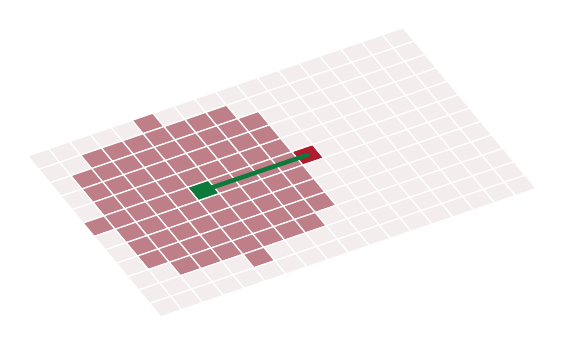
\begin{tikzpicture}
    \begin{axis}[land3d, land view={-28}{40}{0.30},
                 colormap name=htiles, point meta min=0, point meta max=3]
      \addplot3[surf, shader=flat corner, draw=white, line width=0.45pt,
                samples=19, samples y=13, domain=0:18, y domain=0:12,
                point meta={
                  and(abs(x+0.5-\cSx)<0.1, abs(y+0.5-\cSy)<0.1) ? 2 :
                  (and(abs(x+0.5-\cGx)<0.1, abs(y+0.5-\cGy)<0.1) ? 3 :
                  (veclen(x+0.5-\cSx, y+0.5-\cSy) <= \cCost ? 1 : 0))}]
        {0};
      \draw[edgpath, line width=1.6pt, line cap=round] (\cSx,\cSy,0) -- (\cGx,\cGy,0);
    \end{axis}
  \end{tikzpicture}
  &
  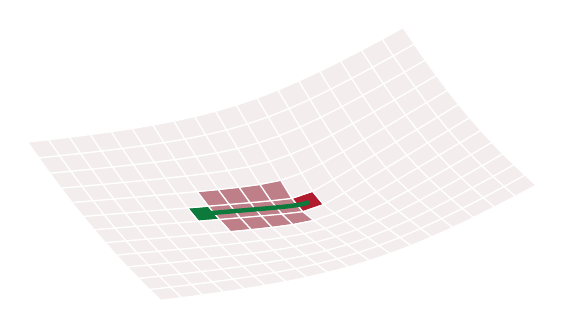
\begin{tikzpicture}
    \begin{axis}[land3d, land view={-28}{40}{0.30},
                 colormap name=htiles, point meta min=0, point meta max=3]
      \addplot3[surf, shader=flat corner, draw=white, line width=0.45pt,
                z buffer=sort, samples=19, samples y=13, domain=0:18, y domain=0:12,
                point meta={
                  and(abs(x+0.5-\cSx)<0.1, abs(y+0.5-\cSy)<0.1) ? 2 :
                  (and(abs(x+0.5-\cGx)<0.1, abs(y+0.5-\cGy)<0.1) ? 3 :
                  (veclen(x+0.5-\cSx, y+0.5-\cSy)
                   + veclen(x+0.5-\cGx, y+0.5-\cGy) <= \cCost+\cSlack ? 1 : 0))}]
        {\kC*veclen(x-\cGx, y-\cGy)};
      \addplot3[edgpath, line width=1.6pt, line cap=round,
                domain=\cSx:\cGx, samples=21, samples y=1]
        ({x}, {\cSy}, {\kC*sqrt((x-\cGx)^2+0.25)});
    \end{axis}
  \end{tikzpicture}\\
  {\scriptsize the search grows as a disk} & {\scriptsize the search is a thin ellipse from $s$ to $t$}\\[4pt]
  \multicolumn{2}{c}{\legendC}
\end{tabular}

  \caption{A schematic comparison on one grid. With the zero heuristic the
    expanded cells form a disk around $s$; with the Euclidean heuristic they
    form a thin ellipse from $s$ to $t$.}\label{fig:funnel}
\end{figure}

\subsection{Experiment: a grid with a U-shaped wall}\label{sec:grid}

An obstacle tests how A* copes with information that its heuristic does not
contain. The instance is as follows (Figure~\ref{fig:grid3d}).

\begin{description}[font=\normalfont\itshape, leftmargin=1.5em, labelindent=0pt]
    \item[Graph.] The 139 free cells of a $16 \times 10$ grid; moves go up, down,
    left or right and cost 1.
  \item[Wall.] A U of 21 cells opening toward the source: column 12, rows 3--7,
    and rows 3 and 7, columns 4--12.
  \item[Query.] From $s = (1,4)$ to $t = (14,6)$, behind the wall, with the
    Manhattan distance as heuristic.
\end{description}

Ties are broken first in, first out. Table~\ref{tab:grid-compare},
Figure~\ref{fig:grid-bars} and Figure~\ref{fig:grid-panels} give the results.

\begin{figure}[htbp]
  \centering
  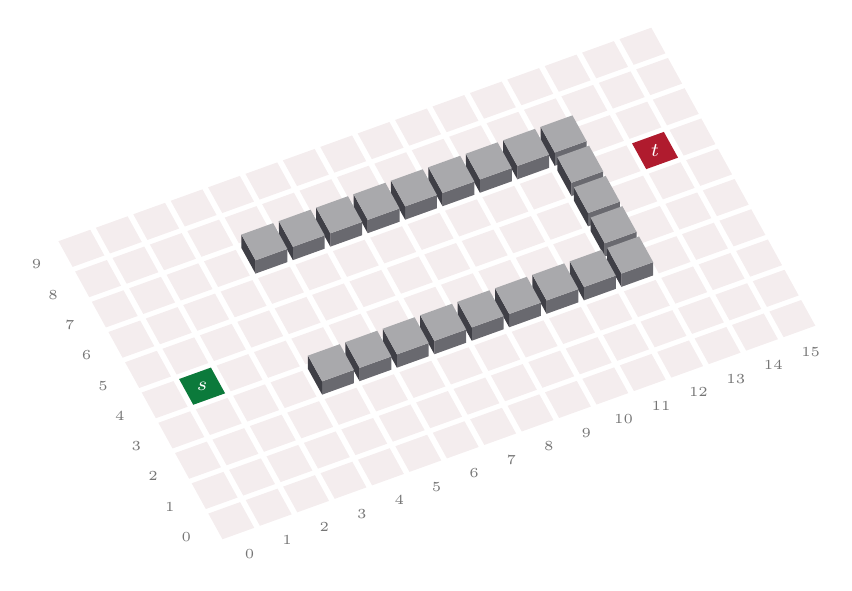
\begin{tikzpicture}[cam={-24}{54}{0.52}{0.52}, line cap=round, line join=round]
  \gfloorthree
  \gendsthree
  \foreach \c in {0,...,15}{\node[tag, text=neutralg, font=\tiny] at ({\c+0.5},-0.6,0) {\c};}
  \foreach \r in {0,...,9}{\node[tag, text=neutralg, font=\tiny] at (-0.7,{\r+0.5},0) {\r};}
  \gwallsthree
\end{tikzpicture}

  \caption{The $16 \times 10$ test grid. The raised blocks form the U-shaped
    wall; the source $s$ is green and the destination $t$ is red.}\label{fig:grid3d}
\end{figure}

\begin{table}[htbp]
  \centering
  \caption{The three algorithms on the grid with the U-shaped
    wall.}\label{tab:grid-compare}
  \begin{tabular}{@{}lccc@{}}
    \toprule
     & \textcolor{algdijkstra}{\textbf{Dijkstra's algorithm}}
     & \textcolor{alggreedy}{\textbf{Greedy best-first}}
     & \textcolor{algastar}{\textbf{A* search}}\\
    \midrule
    Cells expanded (of 139 free) & 137 & 48 & 81\\
    Path cost (moves)            & 19 & 35 & 19\\
    Extra moves over the optimum & 0 & 16 & 0\\
    Shortest path                & \textcolor{algastar}{yes}
                                 & \textcolor{cbRed}{no}
                                 & \textcolor{algastar}{yes}\\
    \bottomrule
  \end{tabular}
\end{table}

\begin{figure}[htbp]
  \centering
  \resultbars{Cells expanded}{165}{137}{48}{81}{0}\hfill
  \resultbars{Path cost (moves)}{42}{19}{35}{19}{19}
  \caption{The results of Table~\ref{tab:grid-compare} as bar charts. The dashed
    line marks the optimal cost.}\label{fig:grid-bars}
\end{figure}

\begin{figure}[htbp]
  \centering
  \renewcommand{\gridpanel}[3]{%
  \begin{tikzpicture}[cam={-24}{54}{0.30}{0.30}, line cap=round, line join=round]
    \foreach \c in {0,...,15}{\foreach \r in {0,...,9}{%
      \ifcsname #1-\c-\r\endcsname \ptile{gclose}{\c}{\r}%
      \else \ptile{gfree}{\c}{\r}\fi}}
    \ptile{gstart}{1}{4}\ptile{ggoal}{14}{6}
    \draw[#3, line width=1.4pt] #2;
    \gwallsthree
  \end{tikzpicture}}
\begin{subfigure}[t]{0.32\textwidth}\centering
  \resizebox{\linewidth}{!}{\gridpanel{dj}{\dijkstraroute}{cbGreen}}
  \caption{Dijkstra's algorithm: 137 cells expanded, path cost 19.}\label{fig:grid-dijkstra}
\end{subfigure}\hfill
\begin{subfigure}[t]{0.32\textwidth}\centering
  \resizebox{\linewidth}{!}{\gridpanel{gr}{\greedyroute}{cbOrange}}
  \caption{Greedy best-first search: 48 cells expanded, path cost 35.}\label{fig:grid-greedy}
\end{subfigure}\hfill
\begin{subfigure}[t]{0.32\textwidth}\centering
  \resizebox{\linewidth}{!}{\gridpanel{as}{\astarroute}{cbGreen}}
  \caption{A* search: 81 cells expanded, path cost 19.}\label{fig:grid-astar}
\end{subfigure}

  \caption{The three algorithms on the grid. Dark tiles were expanded, and the
    line is the returned path.}\label{fig:grid-panels}
\end{figure}

Dijkstra's algorithm expands almost the whole grid. Greedy best-first search
fills the inside of the U and returns a path 16 moves longer than necessary.

A* is also drawn into the U, because the Manhattan distance ignores the wall.
Every cell inside the U is reached by moves toward the destination, so its key
equals $h(s) = 15 < 19 = C^{*}$, and Proposition~\ref{prop:expanded} forces A*
to expand it. A* then goes around the wall and returns a shortest path, after
81 expansions, all among the 137 of Dijkstra's algorithm
(Corollary~\ref{cor:subset}).

Figure~\ref{fig:timeview} raises every cell to the step at which it was
expanded: Dijkstra's algorithm spreads evenly from $s$, whereas A* first fills
the U and then climbs a narrow staircase around the wall.

\begin{figure}[htbp]
  \centering
  \begin{tabular}{@{}c@{\hspace{1em}}c@{}}
  {\footnotesize\textbf{Dijkstra}: 137 expansions} &
  {\footnotesize\textcolor{cbGreen}{\textbf{A*}}: 81 expansions, same scale}\\[2pt]
  \timeview{dj} & \timeview{as}
\end{tabular}

  \caption{Every expanded cell raised to the step at which it was expanded, on
    the same scale in both panels.}\label{fig:timeview}
\end{figure}

\section{Worked example on a real map: Dhaka to Sylhet}\label{sec:casestudy}

We now follow the three algorithms from Dhaka to Sylhet on a map of
Bangladesh.

\subsection{The district graph}\label{sec:mapgraph}

The instance is as follows (Figure~\ref{fig:mapgraph}).

\begin{description}[font=\normalfont\itshape, leftmargin=1.5em, labelindent=0pt]
    \item[Graph.] The 64 districts of Bangladesh, placed at their centres, with
    133 edges between neighboring districts.
  \item[Weights.] The great-circle distance $d(u,v)$ between district centres,
    that is, the shortest distance along the Earth's surface, computed with the
    haversine formula.\footnote{For two points with latitudes $\varphi_1,
    \varphi_2$ and longitudes $\lambda_1, \lambda_2$ on a sphere of radius
    $R$, the haversine formula gives the distance
    $d = 2R \arcsin \sqrt{\sin^2\bigl((\varphi_2 - \varphi_1)/2\bigr) + \cos \varphi_1
    \cos \varphi_2 \sin^2\bigl((\lambda_2 - \lambda_1)/2\bigr)}$; we use
    $R = 6371$\,km.}
\end{description}

The heuristic is the straight-line distance to Sylhet,
\begin{equation}\label{eq:hmap}
  h(v) = d(v, \text{Sylhet}),
\end{equation}
which is consistent because the weights are themselves straight-line distances
(Table~\ref{tab:which-h}).

\begin{figure}[htbp]
  \centering
  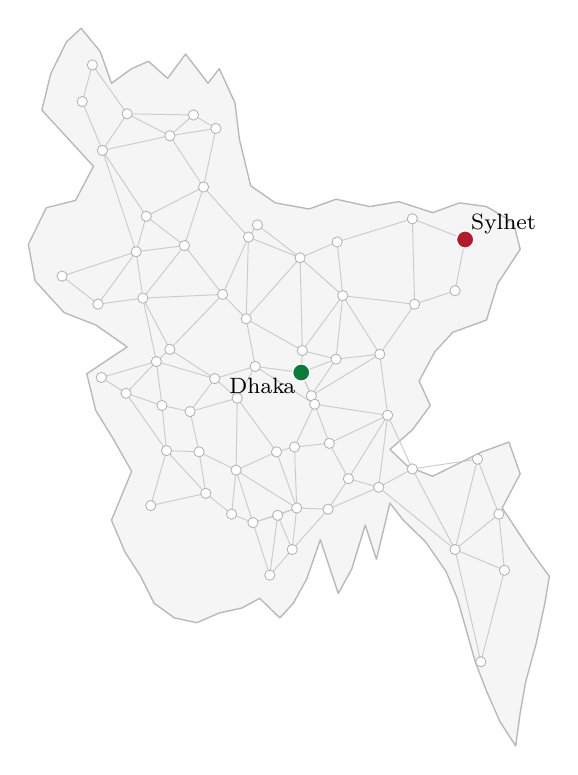
\begin{tikzpicture}[x=1.426cm, y=1.550cm]
  \fill[maplandfill] (0.320,5.820) -- (0.450,5.930) -- (0.620,5.740) -- (0.720,5.480) -- (0.900,5.600) -- (1.050,5.660) -- (1.220,5.520) -- (1.380,5.720) -- (1.580,5.480) -- (1.680,5.600) -- (1.820,5.320) -- (1.860,5.020) -- (1.960,4.640) -- (2.180,4.500) -- (2.480,4.450) -- (2.720,4.530) -- (3.020,4.470) -- (3.280,4.510) -- (3.580,4.420) -- (3.820,4.500) -- (4.060,4.470) -- (4.300,4.340) -- (4.360,4.120) -- (4.160,3.840) -- (4.060,3.540) -- (3.760,3.440) -- (3.600,3.280) -- (3.460,3.040) -- (3.560,2.840) -- (3.400,2.640) -- (3.200,2.480) -- (3.360,2.340) -- (3.580,2.260) -- (4.020,2.460) -- (4.260,2.540) -- (4.360,2.280) -- (4.200,2.000) -- (4.460,1.640) -- (4.620,1.440) -- (4.580,1.220) -- (4.500,0.880) -- (4.410,0.580) -- (4.360,0.320) -- (4.320,0.050) -- (4.180,0.250) -- (4.060,0.500) -- (3.960,0.740) -- (3.880,1.000) -- (3.800,1.260) -- (3.700,1.480) -- (3.520,1.720) -- (3.320,1.900) -- (3.200,2.040) -- (3.080,1.580) -- (2.980,1.860) -- (2.860,1.500) -- (2.740,1.300) -- (2.580,1.740) -- (2.460,1.420) -- (2.340,1.220) -- (2.220,1.100) -- (2.040,1.260) -- (1.880,1.180) -- (1.680,1.140) -- (1.480,1.060) -- (1.280,1.100) -- (1.100,1.220) -- (0.980,1.440) -- (0.840,1.640) -- (0.720,1.900) -- (0.900,2.300) -- (0.740,2.560) -- (0.580,2.800) -- (0.500,3.100) -- (0.860,3.320) -- (0.580,3.500) -- (0.300,3.600) -- (0.040,3.860) -- (-0.020,4.160) -- (0.140,4.460) -- (0.400,4.520) -- (0.560,4.800) -- (0.300,5.060) -- (0.100,5.260) -- (0.180,5.560) -- cycle;
  \draw[mapborder] (0.320,5.820) -- (0.450,5.930) -- (0.620,5.740) -- (0.720,5.480) -- (0.900,5.600) -- (1.050,5.660) -- (1.220,5.520) -- (1.380,5.720) -- (1.580,5.480) -- (1.680,5.600) -- (1.820,5.320) -- (1.860,5.020) -- (1.960,4.640) -- (2.180,4.500) -- (2.480,4.450) -- (2.720,4.530) -- (3.020,4.470) -- (3.280,4.510) -- (3.580,4.420) -- (3.820,4.500) -- (4.060,4.470) -- (4.300,4.340) -- (4.360,4.120) -- (4.160,3.840) -- (4.060,3.540) -- (3.760,3.440) -- (3.600,3.280) -- (3.460,3.040) -- (3.560,2.840) -- (3.400,2.640) -- (3.200,2.480) -- (3.360,2.340) -- (3.580,2.260) -- (4.020,2.460) -- (4.260,2.540) -- (4.360,2.280) -- (4.200,2.000) -- (4.460,1.640) -- (4.620,1.440) -- (4.580,1.220) -- (4.500,0.880) -- (4.410,0.580) -- (4.360,0.320) -- (4.320,0.050) -- (4.180,0.250) -- (4.060,0.500) -- (3.960,0.740) -- (3.880,1.000) -- (3.800,1.260) -- (3.700,1.480) -- (3.520,1.720) -- (3.320,1.900) -- (3.200,2.040) -- (3.080,1.580) -- (2.980,1.860) -- (2.860,1.500) -- (2.740,1.300) -- (2.580,1.740) -- (2.460,1.420) -- (2.340,1.220) -- (2.220,1.100) -- (2.040,1.260) -- (1.880,1.180) -- (1.680,1.140) -- (1.480,1.060) -- (1.280,1.100) -- (1.100,1.220) -- (0.980,1.440) -- (0.840,1.640) -- (0.720,1.900) -- (0.900,2.300) -- (0.740,2.560) -- (0.580,2.800) -- (0.500,3.100) -- (0.860,3.320) -- (0.580,3.500) -- (0.300,3.600) -- (0.040,3.860) -- (-0.020,4.160) -- (0.140,4.460) -- (0.400,4.520) -- (0.560,4.800) -- (0.300,5.060) -- (0.100,5.260) -- (0.180,5.560) -- cycle;
  \coordinate (panchagarh) at (0.550,5.630);
  \coordinate (thakurgaon) at (0.460,5.330);
  \coordinate (nilphamari) at (0.860,5.230);
  \coordinate (lalmonirhat) at (1.450,5.220);
  \coordinate (kurigram) at (1.650,5.110);
  \coordinate (rangpur) at (1.240,5.050);
  \coordinate (dinajpur) at (0.640,4.930);
  \coordinate (gaibandha) at (1.540,4.630);
  \coordinate (joypurhat) at (1.030,4.390);
  \coordinate (sunamganj) at (3.400,4.370);
  \coordinate (sherpur) at (2.020,4.320);
  \coordinate (jamalpur) at (1.940,4.220);
  \coordinate (sylhet) at (3.870,4.200);
  \coordinate (netrokona) at (2.730,4.180);
  \coordinate (bogura) at (1.370,4.150);
  \coordinate (naogaon) at (0.940,4.100);
  \coordinate (mymensingh) at (2.400,4.050);
  \coordinate (chapainawabganj) at (0.280,3.900);
  \coordinate (moulvibazar) at (3.780,3.780);
  \coordinate (sirajganj) at (1.710,3.750);
  \coordinate (kishoreganj) at (2.780,3.740);
  \coordinate (natore) at (1.000,3.720);
  \coordinate (rajshahi) at (0.600,3.670);
  \coordinate (habiganj) at (3.420,3.670);
  \coordinate (tangail) at (1.920,3.550);
  \coordinate (pabna) at (1.240,3.300);
  \coordinate (gazipur) at (2.420,3.290);
  \coordinate (brahmanbaria) at (3.110,3.260);
  \coordinate (narsingdi) at (2.720,3.220);
  \coordinate (kushtia) at (1.120,3.200);
  \coordinate (manikganj) at (2.000,3.160);
  \coordinate (dhaka) at (2.410,3.110);
  \coordinate (meherpur) at (0.630,3.070);
  \coordinate (rajbari) at (1.640,3.060);
  \coordinate (chuadanga) at (0.850,2.940);
  \coordinate (narayanganj) at (2.500,2.920);
  \coordinate (faridpur) at (1.840,2.900);
  \coordinate (munshiganj) at (2.530,2.850);
  \coordinate (jhenaidah) at (1.170,2.840);
  \coordinate (magura) at (1.420,2.790);
  \coordinate (cumilla) at (3.180,2.760);
  \coordinate (chandpur) at (2.660,2.530);
  \coordinate (shariatpur) at (2.350,2.500);
  \coordinate (jashore) at (1.210,2.470);
  \coordinate (narail) at (1.500,2.460);
  \coordinate (madaripur) at (2.190,2.460);
  \coordinate (khagrachhari) at (3.980,2.400);
  \coordinate (feni) at (3.400,2.320);
  \coordinate (gopalganj) at (1.830,2.310);
  \coordinate (lakshmipur) at (2.830,2.240);
  \coordinate (noakhali) at (3.100,2.170);
  \coordinate (khulna) at (1.560,2.120);
  \coordinate (satkhira) at (1.070,2.020);
  \coordinate (barishal) at (2.370,2.000);
  \coordinate (bhola) at (2.650,1.990);
  \coordinate (bagerhat) at (1.790,1.950);
  \coordinate (rangamati) at (4.170,1.950);
  \coordinate (jhalokati) at (2.200,1.940);
  \coordinate (pirojpur) at (1.980,1.880);
  \coordinate (patuakhali) at (2.330,1.660);
  \coordinate (chattogram) at (3.780,1.660);
  \coordinate (bandarban) at (4.220,1.490);
  \coordinate (barguna) at (2.130,1.450);
  \coordinate (coxsbazar) at (4.010,0.740);
  \foreach \a/\b in {panchagarh/thakurgaon, panchagarh/nilphamari, thakurgaon/dinajpur, nilphamari/dinajpur, nilphamari/rangpur, nilphamari/lalmonirhat, lalmonirhat/rangpur, lalmonirhat/kurigram, dinajpur/rangpur, dinajpur/joypurhat, dinajpur/naogaon, rangpur/kurigram, rangpur/gaibandha, kurigram/gaibandha, gaibandha/bogura, gaibandha/joypurhat, gaibandha/jamalpur, joypurhat/naogaon, joypurhat/bogura, naogaon/bogura, naogaon/natore, naogaon/chapainawabganj, naogaon/rajshahi, chapainawabganj/rajshahi, rajshahi/natore, natore/bogura, natore/sirajganj, natore/pabna, natore/kushtia, bogura/sirajganj, sirajganj/pabna, sirajganj/tangail, sirajganj/jamalpur, pabna/kushtia, pabna/rajbari, kushtia/chuadanga, kushtia/jhenaidah, kushtia/meherpur, kushtia/rajbari, meherpur/chuadanga, chuadanga/jhenaidah, chuadanga/jashore, jhenaidah/magura, jhenaidah/jashore, magura/narail, magura/faridpur, magura/rajbari, narail/jashore, narail/khulna, narail/gopalganj, jashore/satkhira, jashore/khulna, satkhira/khulna, khulna/bagerhat, bagerhat/pirojpur, bagerhat/gopalganj, gopalganj/faridpur, gopalganj/madaripur, gopalganj/pirojpur, gopalganj/barishal, rajbari/faridpur, rajbari/manikganj, faridpur/madaripur, faridpur/manikganj, madaripur/shariatpur, madaripur/barishal, shariatpur/chandpur, shariatpur/munshiganj, shariatpur/barishal, pirojpur/jhalokati, pirojpur/barguna, pirojpur/barishal, jhalokati/barishal, jhalokati/barguna, jhalokati/patuakhali, barguna/patuakhali, patuakhali/barishal, patuakhali/bhola, barishal/bhola, bhola/lakshmipur, bhola/noakhali, lakshmipur/noakhali, lakshmipur/chandpur, lakshmipur/cumilla, noakhali/cumilla, noakhali/feni, noakhali/chattogram, feni/cumilla, feni/chattogram, feni/khagrachhari, chandpur/cumilla, chandpur/munshiganj, cumilla/brahmanbaria, cumilla/munshiganj, brahmanbaria/narsingdi, brahmanbaria/kishoreganj, brahmanbaria/habiganj, brahmanbaria/narayanganj, narsingdi/kishoreganj, narsingdi/gazipur, narsingdi/narayanganj, narsingdi/dhaka, munshiganj/narayanganj, munshiganj/dhaka, munshiganj/manikganj, narayanganj/dhaka, dhaka/gazipur, dhaka/manikganj, gazipur/tangail, gazipur/mymensingh, gazipur/kishoreganj, manikganj/tangail, tangail/jamalpur, tangail/mymensingh, jamalpur/sherpur, jamalpur/mymensingh, sherpur/mymensingh, mymensingh/netrokona, mymensingh/kishoreganj, netrokona/kishoreganj, netrokona/sunamganj, kishoreganj/habiganj, habiganj/sunamganj, habiganj/moulvibazar, sunamganj/sylhet, sylhet/moulvibazar, khagrachhari/rangamati, khagrachhari/chattogram, rangamati/chattogram, rangamati/bandarban, bandarban/chattogram, bandarban/coxsbazar, chattogram/coxsbazar}
    {\draw[mapedge] (\a) -- (\b);}
  \foreach \n in {panchagarh, thakurgaon, nilphamari, lalmonirhat, kurigram, rangpur, dinajpur, gaibandha, joypurhat, sunamganj, sherpur, jamalpur, sylhet, netrokona, bogura, naogaon, mymensingh, chapainawabganj, moulvibazar, sirajganj, kishoreganj, natore, rajshahi, habiganj, tangail, pabna, gazipur, brahmanbaria, narsingdi, kushtia, manikganj, dhaka, meherpur, rajbari, chuadanga, narayanganj, faridpur, munshiganj, jhenaidah, magura, cumilla, chandpur, shariatpur, jashore, narail, madaripur, khagrachhari, feni, gopalganj, lakshmipur, noakhali, khulna, satkhira, barishal, bhola, bagerhat, rangamati, jhalokati, pirojpur, patuakhali, chattogram, bandarban, barguna, coxsbazar}
    {\node[mapdot] at (\n) {};}
  \node[mapstart] at (dhaka) {};
  \node[mapgoal] at (sylhet) {};
  \node[maplabel, anchor=north east] at (dhaka) {Dhaka};
  \node[maplabel, anchor=south west] at (sylhet) {Sylhet};
\end{tikzpicture}

  \caption{The district graph: 64 districts of Bangladesh joined by 133 edges
    between neighbors. The source, Dhaka, is green, and the destination, Sylhet, is
    red.}\label{fig:mapgraph}
\end{figure}

\subsection{Dijkstra's algorithm}\label{sec:map-dijkstra}

Dijkstra's algorithm returns the optimal 215.1\,km route but expands 50 of the
64 districts (Figure~\ref{fig:dijkstra-tree}, Table~\ref{tab:dijkstra-result}).
Jashore and Naogaon lie away from Sylhet but are expanded first because they are
closer to Dhaka (Remark~\ref{rem:dijkstra}).

\begin{figure}[htbp]
  \centering
  \begin{tikzpicture}[cam={18}{28}{1.0}{1.09}, line cap=round, line join=round,
                    every node/.style={inner sep=0pt}]
  \def\kz{0.0098}
  \bdfloor
  \lifttree{2}{dhaka/gazipur, dhaka/narayanganj, dhaka/munshiganj, dhaka/narsingdi,
               dhaka/manikganj, munshiganj/chandpur, narsingdi/brahmanbaria,
               munshiganj/shariatpur, manikganj/faridpur, gazipur/tangail}
  \lifttree{3}{manikganj/rajbari, gazipur/kishoreganj, shariatpur/madaripur,
               munshiganj/cumilla, gazipur/mymensingh, chandpur/lakshmipur,
               tangail/sirajganj, rajbari/magura, rajbari/pabna, brahmanbaria/habiganj}
  \lifttree{4}{shariatpur/barishal, kishoreganj/netrokona, madaripur/gopalganj,
               lakshmipur/noakhali, rajbari/kushtia, lakshmipur/bhola,
               magura/jhenaidah, barishal/jhalokati, cumilla/feni, tangail/jamalpur}
  \lifttree{5}{mymensingh/sherpur, magura/narail, sirajganj/bogura,
               habiganj/moulvibazar, barishal/patuakhali, gopalganj/bagerhat,
               barishal/pirojpur, kushtia/chuadanga, sirajganj/natore, narail/jashore}
  \lifttree{6}{kushtia/meherpur, narail/khulna, patuakhali/barguna,
               netrokona/sunamganj, bogura/joypurhat, bogura/naogaon,
               feni/khagrachhari, jamalpur/gaibandha, moulvibazar/sylhet}
  \draw[edgpath, line width=1.8pt] \bdup{dhaka} -- \bdup{narsingdi}
    -- \bdup{brahmanbaria} -- \bdup{habiganj} -- \bdup{moulvibazar}
    -- \bdup{sylhet};
  \node[liftnode, fill=crimson] at \bdup{jashore} {};
  \node[liftnode, fill=crimson] at \bdup{naogaon} {};
  \node[tagbox, text=crimson, anchor=east, xshift=-3pt] at \bdup{jashore} {Jashore 185};
  \node[tagbox, text=crimson, anchor=east, xshift=-3pt] at \bdup{naogaon} {Naogaon 209};
  \node[sball, minimum size=2.4mm] at (dhaka) {};
  \node[tag, text=gstart, anchor=north, yshift=-3pt] at (dhaka) {\textbf{Dhaka}};
  \node[gball, minimum size=2.4mm] at \bdup{sylhet} {};
  \node[tag, text=ggoal, anchor=west, xshift=4pt] at \bdup{sylhet} {\textbf{Sylhet 215}};
\end{tikzpicture}

  \caption{The search tree of Dijkstra's algorithm from Dhaka, with every
    expanded district lifted to its cost $g$ in kilometres. The tree grows in
    every direction; Jashore and Naogaon lie away from Sylhet but are expanded
    before it.}\label{fig:dijkstra-tree}
\end{figure}

\begin{table}[htbp]
  \centering
  \caption{Dijkstra's algorithm from Dhaka to Sylhet.}\label{tab:dijkstra-result}
  \begin{tabular}{@{}ll@{}}
    \toprule
    Districts expanded & 50 of 64\\
    Districts on the route & 6\\
    Route & Dhaka, Narsingdi, Brahmanbaria, Habiganj, Moulvibazar, Sylhet\\
    Route cost & 215.1\,km (optimal)\\
    \bottomrule
  \end{tabular}
\end{table}

\subsection{Greedy best-first search}\label{sec:map-greedy}

Greedy best-first search rolls down the funnel of $h$
(Figure~\ref{fig:greedy-compass}). It expands only six districts, but its route
is 28.1\,km (13\%) longer than the optimum.

\begin{figure}[htbp]
  \centering
  \begin{tikzpicture}[cam={20}{30}{0.96}{1.05}, line cap=round, line join=round,
                    every node/.style={inner sep=0pt}]
  \def\kz{0.0068}
  \def\sx{3.89}\def\sy{4.15}
  \begin{scope}[bdedge/.style={draw=none},
                bdcity/.style={circle, fill=gridgray, minimum size=0.7mm,
                               inner sep=0pt}]\bdfloor\end{scope}
  \foreach \a in {165,200,235,270}{%
    \draw[cbOrange!30, line width=0.4pt] (\sx,\sy,0)
      -- ({\sx+390/101.7*cos(\a)},{\sy+390/111.2*sin(\a)},{390*\kz});}
  \foreach \r in {100,200,300}{%
    \draw[cbOrange!55, line width=0.5pt] plot[domain=150:290, samples=48]
      ({\sx+\r/101.7*cos(\x)},{\sy+\r/111.2*sin(\x)},{\r*\kz});
    \node[tag, text=cbOrange!85!black, anchor=south east, xshift=-1pt]
      at ({\sx+\r/101.7*cos(150)},{\sy+\r/111.2*sin(150)},{\r*\kz}) {$h=\r$};}
  \foreach \n/\vg/\vh in \bddata {%
    \draw[cbOrange!22, line width=0.3pt] (\n) -- \bdlift{\n}{\vh};
    \node[circle, fill=cbOrange!55, minimum size=1.1mm] at \bdlift{\n}{\vh} {};}
  \foreach \a/\b in {dhaka/narsingdi, narsingdi/kishoreganj,
      kishoreganj/habiganj, habiganj/moulvibazar, moulvibazar/sylhet}{%
    \draw[edgorange, line width=1.8pt] \bdlift{\a}{\bdH{\a}} -- \bdlift{\b}{\bdH{\b}};
    \node[circle, fill=cbOrange, draw=white, line width=0.4pt, minimum size=2mm]
      at \bdlift{\b}{\bdH{\b}} {};}
  \node[sball, minimum size=2.4mm] at \bdlift{dhaka}{\bdH{dhaka}} {};
  \node[tagbox, text=gstart, anchor=east, xshift=-4pt]
    at \bdlift{dhaka}{\bdH{dhaka}} {Dhaka, $h=191$};
  \node[gball, minimum size=2.4mm] at (sylhet) {};
  \node[tagbox, text=ggoal, anchor=north, yshift=-4pt] at (sylhet) {Sylhet, $h=0$};
\end{tikzpicture}

  \caption{Every district lifted to $h$, its straight-line distance to Sylhet in
    kilometres. Greedy best-first search (orange) always moves to the lowest
    district it has seen.}\label{fig:greedy-compass}
\end{figure}

The wrong turn is at Narsingdi (Figure~\ref{fig:narsingdi}): Kishoreganj looks
8.4\,km closer to Sylhet, but the road to it is 18.2\,km longer. The key of A*
prefers Brahmanbaria (203.5\,km against 213.3\,km). The two routes differ in
this one district (Figure~\ref{fig:route-flow}).

\begin{figure}[htbp]
  \centering
  \begin{minipage}[c]{0.54\textwidth}\centering
    \resizebox{\linewidth}{!}{\begin{tikzpicture}[cam={20}{40}{3.3}{3.64}, line cap=round, line join=round,
                    every node/.style={inner sep=0pt}]
  \def\kz{0.0047}
  \nefloor
  \draw[edgpath, line width=1.6pt] (dhaka) -- (narsingdi);
  \draw[edgorange, line width=1.4pt] (narsingdi) -- (kishoreganj) -- (habiganj)
    -- (moulvibazar) -- (sylhet);
  \draw[edgpath, line width=1.4pt] (narsingdi) -- (brahmanbaria) -- (habiganj);
  \node[wlab, fill=black!2] at ($(narsingdi)!0.5!(kishoreganj)+(-0.08,0,0)$) {58.1};
  \node[wlab, fill=black!2] at ($(narsingdi)!0.5!(brahmanbaria)+(0,0.065,0)$) {39.9};
  \node[wlab, fill=black!2, text=cbGreen] at ($(dhaka)!0.5!(narsingdi)+(-0.02,0.07,0)$) {33.8};
  \prism{kishoreganj}{0}{91.9}{cbGreen}
  \prism{kishoreganj}{91.9}{213.3}{cbOrange}
  \prism{brahmanbaria}{0}{73.7}{cbGreen}
  \prism{brahmanbaria}{73.7}{203.5}{cbOrange}
  \node[tagbox, anchor=south, yshift=2pt] at \bdlift{kishoreganj}{213.3} {$f=213.3$};
  \node[tagbox, anchor=south, yshift=2pt] at \bdlift{brahmanbaria}{203.5} {$f=\mathbf{203.5}$};
  \node[sball, minimum size=2.4mm] at (dhaka) {};
  \node[cball, minimum size=2.6mm] at (narsingdi) {};
  \node[oball] at (kishoreganj) {};
  \node[oball] at (brahmanbaria) {};
  \node[gball, minimum size=2.4mm] at (sylhet) {};
  \node[maplab, anchor=east, xshift=-4pt] at (dhaka) {Dhaka};
  \node[maplab, anchor=north, yshift=-5pt, text=cbOrange!80!black] at (narsingdi) {\textbf{Narsingdi}};
  \node[maplab, anchor=east, xshift=-5pt] at (kishoreganj) {Kishoreganj};
  \node[maplab, anchor=north, yshift=-5pt] at (brahmanbaria) {Brahmanbaria};
  \node[maplab, anchor=north, yshift=-3pt] at (habiganj) {Habiganj};
  \node[maplab, anchor=west, xshift=4pt] at (sylhet) {Sylhet};
\end{tikzpicture}
}
  \end{minipage}\hfill
  \begin{minipage}[c]{0.43\textwidth}\centering
    \captionof{table}{The two roads out of Narsingdi, where $g = 33.8$\,km.
      All values are in kilometres.}\label{tab:narsingdi}
    \footnotesize\setlength{\tabcolsep}{4pt}
    \resizebox{\linewidth}{!}{%
    \begin{tabular}{@{}lcc@{}}
      \toprule
      & Kishoreganj & Brahmanbaria\\
      \midrule
      road from Narsingdi    & 58.1 & 39.9\\
      $h$ to Sylhet          & \textbf{121.4} & 129.8\\
      $g$ through Narsingdi  & 91.9 & 73.7\\
      $f = g + h$            & 213.3 & \textbf{203.5}\\
      \midrule
      chosen by greedy search  & \checkmark & \\
      smaller key $f$ (A*)     & & \checkmark\\
      \bottomrule
    \end{tabular}}
  \end{minipage}
  \caption{The choice at Narsingdi. Each column shows $g$ (green) with $h$
    (orange) on top, so its height is $f$.}\label{fig:narsingdi}
\end{figure}

\begin{figure}[htbp]
  \centering
  \tikzset{
  rbox/.style  = {draw=black!65, fill=white, line width=0.7pt, rounded corners=2pt,
                  minimum width=2.9cm, minimum height=0.55cm, font=\small,
                  inner sep=2pt, text=black},
  rend/.style  = {rbox=#1, fill=gray!18, font=\small\bfseries},
  rarr/.style  = {-{Stealth[length=2mm]}, line width=0.8pt, draw=black!60},
  rleg/.style  = {font=\scriptsize, text=inkgray, right=3pt, midway},
}
\begin{tikzpicture}[x=1cm, y=1cm]
  \node[font=\small\bfseries, text=algastar] at (0,0.75) {Dijkstra and A*};
  \foreach \n/\name/\s in {0/Dhaka/rend, 1/Narsingdi/rbox, 2/Brahmanbaria/rbox,
                           3/Habiganj/rbox, 4/Moulvibazar/rbox, 5/Sylhet/rend}
    {\node[\s=algastar] (d\n) at (0,-0.95*\n) {\name};}
  \foreach \a/\b/\km in {0/1/33.8, 1/2/39.9, 2/3/55.4, 3/4/38.4, 4/5/47.6}
    {\draw[rarr] (d\a) -- node[rleg] {\km\,km} (d\b);}
  \node[font=\small, text=algastar, below=4pt] at (d5.south) {total \textbf{215.1\,km} (optimal)};
  \node[font=\small\bfseries, text=alggreedy] at (6.4,0.75) {Greedy best-first search};
  \foreach \n/\name/\s in {0/Dhaka/rend, 1/Narsingdi/rbox, 2/Kishoreganj/rbox,
                           3/Habiganj/rbox, 4/Moulvibazar/rbox, 5/Sylhet/rend}
    {\node[\s=alggreedy] (g\n) at (6.4,-0.95*\n) {\name};}
  \foreach \a/\b/\km in {0/1/33.8, 1/2/58.1, 2/3/65.3, 3/4/38.4, 4/5/47.6}
    {\draw[rarr] (g\a) -- node[rleg] {\km\,km} (g\b);}
  \node[font=\small, text=alggreedy, below=4pt] at (g5.south) {total \textbf{243.2\,km} (+28.1\,km)};
  \draw[black, line width=1pt, rounded corners=2pt] ($(d2.north west)+(-0.08,0.08)$)
    rectangle ($(d2.south east)+(0.08,-0.08)$);
  \draw[black, line width=1pt, rounded corners=2pt] ($(g2.north west)+(-0.08,0.08)$)
    rectangle ($(g2.south east)+(0.08,-0.08)$);
  \draw[black!70, line width=0.6pt, dashed] ($(d2.east)+(0.08,0)$) -- node[fill=white,
    font=\scriptsize, text=cbRed, inner sep=1pt] {the only difference} ($(g2.west)+(-0.08,0)$);
\end{tikzpicture}

  \caption{The routes from Dhaka to Sylhet as flow charts, with the length of
    every leg.}\label{fig:route-flow}
\end{figure}

\subsection{A* search}\label{sec:map-astar}

A* returns the optimal route after eight expansions
(Figure~\ref{fig:astar-columns}, Table~\ref{tab:astar-map}). The run
illustrates three results of the report:
\begin{enumerate}[label=(\arabic*)]
  \item The off-route districts Gazipur and Kishoreganj are expanded because
    their keys are below $C^{*}$ (Proposition~\ref{prop:expanded}).
  \item Relaxation repairs the detour: Habiganj is first reached through
    Kishoreganj at 147.3\,km and then through Brahmanbaria at 129.1\,km.
  \item The keys never decrease (Lemma~\ref{lem:monotone}).
\end{enumerate}

\begin{figure}[htbp]
  \centering
  \begin{tikzpicture}[cam={20}{40}{3.3}{3.64}, line cap=round, line join=round,
                    every node/.style={inner sep=0pt}]
  \def\kz{0.0047}
  \nefloor
  \foreach \a/\b in {dhaka/narsingdi, dhaka/gazipur, gazipur/kishoreganj,
      narsingdi/brahmanbaria, brahmanbaria/habiganj, habiganj/moulvibazar,
      moulvibazar/sylhet}{\draw[rblue!70, line width=0.9pt] (\a) -- (\b);}
  \draw[edgpath, line width=1.6pt] (dhaka) -- (narsingdi)
    -- (brahmanbaria) -- (habiganj) -- (moulvibazar) -- (sylhet);
  \prism{sylhet}{0}{215.1}{cbGreen}
  \prism{kishoreganj}{0}{82.0}{cbGreen}
  \prism{kishoreganj}{82.0}{203.4}{cbOrange}
  \prism{habiganj}{0}{129.1}{cbGreen}
  \prism{habiganj}{129.1}{203.5}{cbOrange}
  \prism{moulvibazar}{0}{167.5}{cbGreen}
  \prism{moulvibazar}{167.5}{215.1}{cbOrange}
  \prism{gazipur}{0}{20.0}{cbGreen}
  \prism{gazipur}{20.0}{198.3}{cbOrange}
  \prism{narsingdi}{0}{33.8}{cbGreen}
  \prism{narsingdi}{33.8}{193.3}{cbOrange}
  \prism{dhaka}{0}{191.2}{cbOrange}
  \prism{brahmanbaria}{0}{73.7}{cbGreen}
  \prism{brahmanbaria}{73.7}{203.5}{cbOrange}
  \begin{scope}[shift={(-87.98,-20.75,{215.1*\kz})}]
    \draw[cbGreen, line width=0.7pt, dash pattern=on 2.5pt off 1.5pt]
      (90.3,23.7) -- (92.0,23.7) -- (92.0,25.0) -- (90.3,25.0) -- cycle;
    \node[tagbox, text=cbGreen, anchor=south, yshift=2pt]
      at (91.15,25.0) {ceiling $C^{*} = 215.1$\,km};
  \end{scope}
  \node[sball, minimum size=2.4mm] at (dhaka) {};
  \node[gball, minimum size=2.4mm] at (sylhet) {};
  \node[maplab, anchor=north east, xshift=-2pt, yshift=-1pt] at (dhaka) {Dhaka};
  \node[maplab, anchor=west, xshift=4pt] at (sylhet) {Sylhet};
  \node[maplab, anchor=north, yshift=-3pt] at (gazipur) {Gazipur};
  \node[maplab, anchor=east, xshift=-4pt] at (kishoreganj) {Kishoreganj};
\end{tikzpicture}

  \caption{The eight districts expanded by A*, as columns of $g$ (green) and $h$
    (orange). No column rises above the optimal cost $C^{*} = 215.1$\,km
    (dashed).}\label{fig:astar-columns}
\end{figure}

\begin{table}[htbp]
  \centering
  \caption{The districts expanded by A* from Dhaka to Sylhet, in order. All
    values are in kilometres.}\label{tab:astar-map}
  \begin{tabular}{@{}rlrrr@{}}
    \toprule
    Step & District & $g$ & $h$ & $f = g + h$\\
    \midrule
    \inputrows{figures/map_astar_rows.tex}
    \bottomrule
  \end{tabular}
\end{table}

\subsection{Comparison}\label{sec:map-compare}

Table~\ref{tab:map-compare}, Figure~\ref{fig:map-bars} and
Figure~\ref{fig:map-panels} compare the three algorithms.

\begin{table}[htbp]
  \centering
  \caption{The three algorithms on the district graph, from Dhaka to
    Sylhet.}\label{tab:map-compare}
  \begin{tabular}{@{}lccc@{}}
    \toprule
     & \textcolor{algdijkstra}{\textbf{Dijkstra's algorithm}}
     & \textcolor{alggreedy}{\textbf{Greedy best-first}}
     & \textcolor{algastar}{\textbf{A* search}}\\
    \midrule
    Districts expanded (of 64) & 50 & 6 & 8\\
    Route cost (km)            & 215.1 & 243.2 & 215.1\\
    Extra cost over the optimum & 0 & 28.1\,km (13\%) & 0\\
    Shortest route             & \textcolor{algastar}{yes}
                               & \textcolor{cbRed}{no}
                               & \textcolor{algastar}{yes}\\
    \bottomrule
  \end{tabular}
\end{table}

\begin{figure}[htbp]
  \centering
  \resultbars{Districts expanded}{62}{50}{6}{8}{0}\hfill
  \resultbars{Route cost (km)}{290}{215.1}{243.2}{215.1}{215.1}
  \caption{The results of Table~\ref{tab:map-compare} as bar charts. The dashed
    line marks the optimal cost.}\label{fig:map-bars}
\end{figure}

\begin{figure}[htbp]
  \centering
  \begin{subfigure}[t]{0.32\textwidth}\centering
  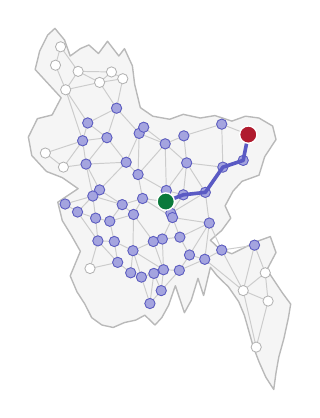
\begin{tikzpicture}[x=0.718cm, y=0.780cm]
    \fill[maplandfill] (0.320,5.820) -- (0.450,5.930) -- (0.620,5.740) -- (0.720,5.480) -- (0.900,5.600) -- (1.050,5.660) -- (1.220,5.520) -- (1.380,5.720) -- (1.580,5.480) -- (1.680,5.600) -- (1.820,5.320) -- (1.860,5.020) -- (1.960,4.640) -- (2.180,4.500) -- (2.480,4.450) -- (2.720,4.530) -- (3.020,4.470) -- (3.280,4.510) -- (3.580,4.420) -- (3.820,4.500) -- (4.060,4.470) -- (4.300,4.340) -- (4.360,4.120) -- (4.160,3.840) -- (4.060,3.540) -- (3.760,3.440) -- (3.600,3.280) -- (3.460,3.040) -- (3.560,2.840) -- (3.400,2.640) -- (3.200,2.480) -- (3.360,2.340) -- (3.580,2.260) -- (4.020,2.460) -- (4.260,2.540) -- (4.360,2.280) -- (4.200,2.000) -- (4.460,1.640) -- (4.620,1.440) -- (4.580,1.220) -- (4.500,0.880) -- (4.410,0.580) -- (4.360,0.320) -- (4.320,0.050) -- (4.180,0.250) -- (4.060,0.500) -- (3.960,0.740) -- (3.880,1.000) -- (3.800,1.260) -- (3.700,1.480) -- (3.520,1.720) -- (3.320,1.900) -- (3.200,2.040) -- (3.080,1.580) -- (2.980,1.860) -- (2.860,1.500) -- (2.740,1.300) -- (2.580,1.740) -- (2.460,1.420) -- (2.340,1.220) -- (2.220,1.100) -- (2.040,1.260) -- (1.880,1.180) -- (1.680,1.140) -- (1.480,1.060) -- (1.280,1.100) -- (1.100,1.220) -- (0.980,1.440) -- (0.840,1.640) -- (0.720,1.900) -- (0.900,2.300) -- (0.740,2.560) -- (0.580,2.800) -- (0.500,3.100) -- (0.860,3.320) -- (0.580,3.500) -- (0.300,3.600) -- (0.040,3.860) -- (-0.020,4.160) -- (0.140,4.460) -- (0.400,4.520) -- (0.560,4.800) -- (0.300,5.060) -- (0.100,5.260) -- (0.180,5.560) -- cycle;
    \draw[mapborder] (0.320,5.820) -- (0.450,5.930) -- (0.620,5.740) -- (0.720,5.480) -- (0.900,5.600) -- (1.050,5.660) -- (1.220,5.520) -- (1.380,5.720) -- (1.580,5.480) -- (1.680,5.600) -- (1.820,5.320) -- (1.860,5.020) -- (1.960,4.640) -- (2.180,4.500) -- (2.480,4.450) -- (2.720,4.530) -- (3.020,4.470) -- (3.280,4.510) -- (3.580,4.420) -- (3.820,4.500) -- (4.060,4.470) -- (4.300,4.340) -- (4.360,4.120) -- (4.160,3.840) -- (4.060,3.540) -- (3.760,3.440) -- (3.600,3.280) -- (3.460,3.040) -- (3.560,2.840) -- (3.400,2.640) -- (3.200,2.480) -- (3.360,2.340) -- (3.580,2.260) -- (4.020,2.460) -- (4.260,2.540) -- (4.360,2.280) -- (4.200,2.000) -- (4.460,1.640) -- (4.620,1.440) -- (4.580,1.220) -- (4.500,0.880) -- (4.410,0.580) -- (4.360,0.320) -- (4.320,0.050) -- (4.180,0.250) -- (4.060,0.500) -- (3.960,0.740) -- (3.880,1.000) -- (3.800,1.260) -- (3.700,1.480) -- (3.520,1.720) -- (3.320,1.900) -- (3.200,2.040) -- (3.080,1.580) -- (2.980,1.860) -- (2.860,1.500) -- (2.740,1.300) -- (2.580,1.740) -- (2.460,1.420) -- (2.340,1.220) -- (2.220,1.100) -- (2.040,1.260) -- (1.880,1.180) -- (1.680,1.140) -- (1.480,1.060) -- (1.280,1.100) -- (1.100,1.220) -- (0.980,1.440) -- (0.840,1.640) -- (0.720,1.900) -- (0.900,2.300) -- (0.740,2.560) -- (0.580,2.800) -- (0.500,3.100) -- (0.860,3.320) -- (0.580,3.500) -- (0.300,3.600) -- (0.040,3.860) -- (-0.020,4.160) -- (0.140,4.460) -- (0.400,4.520) -- (0.560,4.800) -- (0.300,5.060) -- (0.100,5.260) -- (0.180,5.560) -- cycle;
    \coordinate (panchagarh) at (0.550,5.630);
    \coordinate (thakurgaon) at (0.460,5.330);
    \coordinate (nilphamari) at (0.860,5.230);
    \coordinate (lalmonirhat) at (1.450,5.220);
    \coordinate (kurigram) at (1.650,5.110);
    \coordinate (rangpur) at (1.240,5.050);
    \coordinate (dinajpur) at (0.640,4.930);
    \coordinate (gaibandha) at (1.540,4.630);
    \coordinate (joypurhat) at (1.030,4.390);
    \coordinate (sunamganj) at (3.400,4.370);
    \coordinate (sherpur) at (2.020,4.320);
    \coordinate (jamalpur) at (1.940,4.220);
    \coordinate (sylhet) at (3.870,4.200);
    \coordinate (netrokona) at (2.730,4.180);
    \coordinate (bogura) at (1.370,4.150);
    \coordinate (naogaon) at (0.940,4.100);
    \coordinate (mymensingh) at (2.400,4.050);
    \coordinate (chapainawabganj) at (0.280,3.900);
    \coordinate (moulvibazar) at (3.780,3.780);
    \coordinate (sirajganj) at (1.710,3.750);
    \coordinate (kishoreganj) at (2.780,3.740);
    \coordinate (natore) at (1.000,3.720);
    \coordinate (rajshahi) at (0.600,3.670);
    \coordinate (habiganj) at (3.420,3.670);
    \coordinate (tangail) at (1.920,3.550);
    \coordinate (pabna) at (1.240,3.300);
    \coordinate (gazipur) at (2.420,3.290);
    \coordinate (brahmanbaria) at (3.110,3.260);
    \coordinate (narsingdi) at (2.720,3.220);
    \coordinate (kushtia) at (1.120,3.200);
    \coordinate (manikganj) at (2.000,3.160);
    \coordinate (dhaka) at (2.410,3.110);
    \coordinate (meherpur) at (0.630,3.070);
    \coordinate (rajbari) at (1.640,3.060);
    \coordinate (chuadanga) at (0.850,2.940);
    \coordinate (narayanganj) at (2.500,2.920);
    \coordinate (faridpur) at (1.840,2.900);
    \coordinate (munshiganj) at (2.530,2.850);
    \coordinate (jhenaidah) at (1.170,2.840);
    \coordinate (magura) at (1.420,2.790);
    \coordinate (cumilla) at (3.180,2.760);
    \coordinate (chandpur) at (2.660,2.530);
    \coordinate (shariatpur) at (2.350,2.500);
    \coordinate (jashore) at (1.210,2.470);
    \coordinate (narail) at (1.500,2.460);
    \coordinate (madaripur) at (2.190,2.460);
    \coordinate (khagrachhari) at (3.980,2.400);
    \coordinate (feni) at (3.400,2.320);
    \coordinate (gopalganj) at (1.830,2.310);
    \coordinate (lakshmipur) at (2.830,2.240);
    \coordinate (noakhali) at (3.100,2.170);
    \coordinate (khulna) at (1.560,2.120);
    \coordinate (satkhira) at (1.070,2.020);
    \coordinate (barishal) at (2.370,2.000);
    \coordinate (bhola) at (2.650,1.990);
    \coordinate (bagerhat) at (1.790,1.950);
    \coordinate (rangamati) at (4.170,1.950);
    \coordinate (jhalokati) at (2.200,1.940);
    \coordinate (pirojpur) at (1.980,1.880);
    \coordinate (patuakhali) at (2.330,1.660);
    \coordinate (chattogram) at (3.780,1.660);
    \coordinate (bandarban) at (4.220,1.490);
    \coordinate (barguna) at (2.130,1.450);
    \coordinate (coxsbazar) at (4.010,0.740);
    \foreach \a/\b in {panchagarh/thakurgaon, panchagarh/nilphamari, thakurgaon/dinajpur, nilphamari/dinajpur, nilphamari/rangpur, nilphamari/lalmonirhat, lalmonirhat/rangpur, lalmonirhat/kurigram, dinajpur/rangpur, dinajpur/joypurhat, dinajpur/naogaon, rangpur/kurigram, rangpur/gaibandha, kurigram/gaibandha, gaibandha/bogura, gaibandha/joypurhat, gaibandha/jamalpur, joypurhat/naogaon, joypurhat/bogura, naogaon/bogura, naogaon/natore, naogaon/chapainawabganj, naogaon/rajshahi, chapainawabganj/rajshahi, rajshahi/natore, natore/bogura, natore/sirajganj, natore/pabna, natore/kushtia, bogura/sirajganj, sirajganj/pabna, sirajganj/tangail, sirajganj/jamalpur, pabna/kushtia, pabna/rajbari, kushtia/chuadanga, kushtia/jhenaidah, kushtia/meherpur, kushtia/rajbari, meherpur/chuadanga, chuadanga/jhenaidah, chuadanga/jashore, jhenaidah/magura, jhenaidah/jashore, magura/narail, magura/faridpur, magura/rajbari, narail/jashore, narail/khulna, narail/gopalganj, jashore/satkhira, jashore/khulna, satkhira/khulna, khulna/bagerhat, bagerhat/pirojpur, bagerhat/gopalganj, gopalganj/faridpur, gopalganj/madaripur, gopalganj/pirojpur, gopalganj/barishal, rajbari/faridpur, rajbari/manikganj, faridpur/madaripur, faridpur/manikganj, madaripur/shariatpur, madaripur/barishal, shariatpur/chandpur, shariatpur/munshiganj, shariatpur/barishal, pirojpur/jhalokati, pirojpur/barguna, pirojpur/barishal, jhalokati/barishal, jhalokati/barguna, jhalokati/patuakhali, barguna/patuakhali, patuakhali/barishal, patuakhali/bhola, barishal/bhola, bhola/lakshmipur, bhola/noakhali, lakshmipur/noakhali, lakshmipur/chandpur, lakshmipur/cumilla, noakhali/cumilla, noakhali/feni, noakhali/chattogram, feni/cumilla, feni/chattogram, feni/khagrachhari, chandpur/cumilla, chandpur/munshiganj, cumilla/brahmanbaria, cumilla/munshiganj, brahmanbaria/narsingdi, brahmanbaria/kishoreganj, brahmanbaria/habiganj, brahmanbaria/narayanganj, narsingdi/kishoreganj, narsingdi/gazipur, narsingdi/narayanganj, narsingdi/dhaka, munshiganj/narayanganj, munshiganj/dhaka, munshiganj/manikganj, narayanganj/dhaka, dhaka/gazipur, dhaka/manikganj, gazipur/tangail, gazipur/mymensingh, gazipur/kishoreganj, manikganj/tangail, tangail/jamalpur, tangail/mymensingh, jamalpur/sherpur, jamalpur/mymensingh, sherpur/mymensingh, mymensingh/netrokona, mymensingh/kishoreganj, netrokona/kishoreganj, netrokona/sunamganj, kishoreganj/habiganj, habiganj/sunamganj, habiganj/moulvibazar, sunamganj/sylhet, sylhet/moulvibazar, khagrachhari/rangamati, khagrachhari/chattogram, rangamati/chattogram, rangamati/bandarban, bandarban/chattogram, bandarban/coxsbazar, chattogram/coxsbazar}
      {\draw[mapedge] (\a) -- (\b);}
    \foreach \n in {panchagarh, thakurgaon, nilphamari, lalmonirhat, kurigram, rangpur, dinajpur, gaibandha, joypurhat, sunamganj, sherpur, jamalpur, sylhet, netrokona, bogura, naogaon, mymensingh, chapainawabganj, moulvibazar, sirajganj, kishoreganj, natore, rajshahi, habiganj, tangail, pabna, gazipur, brahmanbaria, narsingdi, kushtia, manikganj, dhaka, meherpur, rajbari, chuadanga, narayanganj, faridpur, munshiganj, jhenaidah, magura, cumilla, chandpur, shariatpur, jashore, narail, madaripur, khagrachhari, feni, gopalganj, lakshmipur, noakhali, khulna, satkhira, barishal, bhola, bagerhat, rangamati, jhalokati, pirojpur, patuakhali, chattogram, bandarban, barguna, coxsbazar}
      {\node[mapdot] at (\n) {};}
    \foreach \n in {dhaka, gazipur, narayanganj, munshiganj, narsingdi, manikganj, chandpur, brahmanbaria, shariatpur, faridpur, tangail, rajbari, kishoreganj, madaripur, cumilla, mymensingh, lakshmipur, sirajganj, magura, pabna, habiganj, barishal, netrokona, gopalganj, noakhali, kushtia, bhola, jhenaidah, jhalokati, feni, jamalpur, sherpur, narail, bogura, moulvibazar, patuakhali, bagerhat, pirojpur, chuadanga, natore, jashore, meherpur, khulna, barguna, sunamganj, joypurhat, naogaon, khagrachhari, gaibandha, sylhet}
      {\node[mapdot, fill=algdijkstra!55, draw=algdijkstra] at (\n) {};}
    \draw[maproute, draw=algdijkstra] (dhaka) -- (narsingdi) -- (brahmanbaria) -- (habiganj) -- (moulvibazar) -- (sylhet);
  \node[mapstart] at (dhaka) {};
  \node[mapgoal] at (sylhet) {};
  \end{tikzpicture}
  \caption{Dijkstra's algorithm: 50 districts expanded, route 215.1\,km.}
  \label{fig:map-dijkstra}
\end{subfigure}\hfill
\begin{subfigure}[t]{0.32\textwidth}\centering
  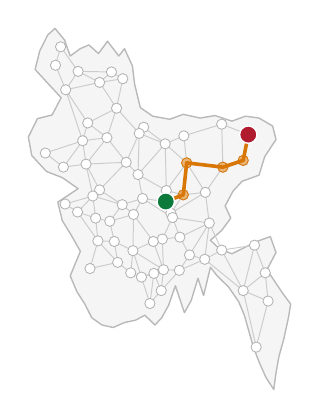
\begin{tikzpicture}[x=0.718cm, y=0.780cm]
    \fill[maplandfill] (0.320,5.820) -- (0.450,5.930) -- (0.620,5.740) -- (0.720,5.480) -- (0.900,5.600) -- (1.050,5.660) -- (1.220,5.520) -- (1.380,5.720) -- (1.580,5.480) -- (1.680,5.600) -- (1.820,5.320) -- (1.860,5.020) -- (1.960,4.640) -- (2.180,4.500) -- (2.480,4.450) -- (2.720,4.530) -- (3.020,4.470) -- (3.280,4.510) -- (3.580,4.420) -- (3.820,4.500) -- (4.060,4.470) -- (4.300,4.340) -- (4.360,4.120) -- (4.160,3.840) -- (4.060,3.540) -- (3.760,3.440) -- (3.600,3.280) -- (3.460,3.040) -- (3.560,2.840) -- (3.400,2.640) -- (3.200,2.480) -- (3.360,2.340) -- (3.580,2.260) -- (4.020,2.460) -- (4.260,2.540) -- (4.360,2.280) -- (4.200,2.000) -- (4.460,1.640) -- (4.620,1.440) -- (4.580,1.220) -- (4.500,0.880) -- (4.410,0.580) -- (4.360,0.320) -- (4.320,0.050) -- (4.180,0.250) -- (4.060,0.500) -- (3.960,0.740) -- (3.880,1.000) -- (3.800,1.260) -- (3.700,1.480) -- (3.520,1.720) -- (3.320,1.900) -- (3.200,2.040) -- (3.080,1.580) -- (2.980,1.860) -- (2.860,1.500) -- (2.740,1.300) -- (2.580,1.740) -- (2.460,1.420) -- (2.340,1.220) -- (2.220,1.100) -- (2.040,1.260) -- (1.880,1.180) -- (1.680,1.140) -- (1.480,1.060) -- (1.280,1.100) -- (1.100,1.220) -- (0.980,1.440) -- (0.840,1.640) -- (0.720,1.900) -- (0.900,2.300) -- (0.740,2.560) -- (0.580,2.800) -- (0.500,3.100) -- (0.860,3.320) -- (0.580,3.500) -- (0.300,3.600) -- (0.040,3.860) -- (-0.020,4.160) -- (0.140,4.460) -- (0.400,4.520) -- (0.560,4.800) -- (0.300,5.060) -- (0.100,5.260) -- (0.180,5.560) -- cycle;
    \draw[mapborder] (0.320,5.820) -- (0.450,5.930) -- (0.620,5.740) -- (0.720,5.480) -- (0.900,5.600) -- (1.050,5.660) -- (1.220,5.520) -- (1.380,5.720) -- (1.580,5.480) -- (1.680,5.600) -- (1.820,5.320) -- (1.860,5.020) -- (1.960,4.640) -- (2.180,4.500) -- (2.480,4.450) -- (2.720,4.530) -- (3.020,4.470) -- (3.280,4.510) -- (3.580,4.420) -- (3.820,4.500) -- (4.060,4.470) -- (4.300,4.340) -- (4.360,4.120) -- (4.160,3.840) -- (4.060,3.540) -- (3.760,3.440) -- (3.600,3.280) -- (3.460,3.040) -- (3.560,2.840) -- (3.400,2.640) -- (3.200,2.480) -- (3.360,2.340) -- (3.580,2.260) -- (4.020,2.460) -- (4.260,2.540) -- (4.360,2.280) -- (4.200,2.000) -- (4.460,1.640) -- (4.620,1.440) -- (4.580,1.220) -- (4.500,0.880) -- (4.410,0.580) -- (4.360,0.320) -- (4.320,0.050) -- (4.180,0.250) -- (4.060,0.500) -- (3.960,0.740) -- (3.880,1.000) -- (3.800,1.260) -- (3.700,1.480) -- (3.520,1.720) -- (3.320,1.900) -- (3.200,2.040) -- (3.080,1.580) -- (2.980,1.860) -- (2.860,1.500) -- (2.740,1.300) -- (2.580,1.740) -- (2.460,1.420) -- (2.340,1.220) -- (2.220,1.100) -- (2.040,1.260) -- (1.880,1.180) -- (1.680,1.140) -- (1.480,1.060) -- (1.280,1.100) -- (1.100,1.220) -- (0.980,1.440) -- (0.840,1.640) -- (0.720,1.900) -- (0.900,2.300) -- (0.740,2.560) -- (0.580,2.800) -- (0.500,3.100) -- (0.860,3.320) -- (0.580,3.500) -- (0.300,3.600) -- (0.040,3.860) -- (-0.020,4.160) -- (0.140,4.460) -- (0.400,4.520) -- (0.560,4.800) -- (0.300,5.060) -- (0.100,5.260) -- (0.180,5.560) -- cycle;
    \coordinate (panchagarh) at (0.550,5.630);
    \coordinate (thakurgaon) at (0.460,5.330);
    \coordinate (nilphamari) at (0.860,5.230);
    \coordinate (lalmonirhat) at (1.450,5.220);
    \coordinate (kurigram) at (1.650,5.110);
    \coordinate (rangpur) at (1.240,5.050);
    \coordinate (dinajpur) at (0.640,4.930);
    \coordinate (gaibandha) at (1.540,4.630);
    \coordinate (joypurhat) at (1.030,4.390);
    \coordinate (sunamganj) at (3.400,4.370);
    \coordinate (sherpur) at (2.020,4.320);
    \coordinate (jamalpur) at (1.940,4.220);
    \coordinate (sylhet) at (3.870,4.200);
    \coordinate (netrokona) at (2.730,4.180);
    \coordinate (bogura) at (1.370,4.150);
    \coordinate (naogaon) at (0.940,4.100);
    \coordinate (mymensingh) at (2.400,4.050);
    \coordinate (chapainawabganj) at (0.280,3.900);
    \coordinate (moulvibazar) at (3.780,3.780);
    \coordinate (sirajganj) at (1.710,3.750);
    \coordinate (kishoreganj) at (2.780,3.740);
    \coordinate (natore) at (1.000,3.720);
    \coordinate (rajshahi) at (0.600,3.670);
    \coordinate (habiganj) at (3.420,3.670);
    \coordinate (tangail) at (1.920,3.550);
    \coordinate (pabna) at (1.240,3.300);
    \coordinate (gazipur) at (2.420,3.290);
    \coordinate (brahmanbaria) at (3.110,3.260);
    \coordinate (narsingdi) at (2.720,3.220);
    \coordinate (kushtia) at (1.120,3.200);
    \coordinate (manikganj) at (2.000,3.160);
    \coordinate (dhaka) at (2.410,3.110);
    \coordinate (meherpur) at (0.630,3.070);
    \coordinate (rajbari) at (1.640,3.060);
    \coordinate (chuadanga) at (0.850,2.940);
    \coordinate (narayanganj) at (2.500,2.920);
    \coordinate (faridpur) at (1.840,2.900);
    \coordinate (munshiganj) at (2.530,2.850);
    \coordinate (jhenaidah) at (1.170,2.840);
    \coordinate (magura) at (1.420,2.790);
    \coordinate (cumilla) at (3.180,2.760);
    \coordinate (chandpur) at (2.660,2.530);
    \coordinate (shariatpur) at (2.350,2.500);
    \coordinate (jashore) at (1.210,2.470);
    \coordinate (narail) at (1.500,2.460);
    \coordinate (madaripur) at (2.190,2.460);
    \coordinate (khagrachhari) at (3.980,2.400);
    \coordinate (feni) at (3.400,2.320);
    \coordinate (gopalganj) at (1.830,2.310);
    \coordinate (lakshmipur) at (2.830,2.240);
    \coordinate (noakhali) at (3.100,2.170);
    \coordinate (khulna) at (1.560,2.120);
    \coordinate (satkhira) at (1.070,2.020);
    \coordinate (barishal) at (2.370,2.000);
    \coordinate (bhola) at (2.650,1.990);
    \coordinate (bagerhat) at (1.790,1.950);
    \coordinate (rangamati) at (4.170,1.950);
    \coordinate (jhalokati) at (2.200,1.940);
    \coordinate (pirojpur) at (1.980,1.880);
    \coordinate (patuakhali) at (2.330,1.660);
    \coordinate (chattogram) at (3.780,1.660);
    \coordinate (bandarban) at (4.220,1.490);
    \coordinate (barguna) at (2.130,1.450);
    \coordinate (coxsbazar) at (4.010,0.740);
    \foreach \a/\b in {panchagarh/thakurgaon, panchagarh/nilphamari, thakurgaon/dinajpur, nilphamari/dinajpur, nilphamari/rangpur, nilphamari/lalmonirhat, lalmonirhat/rangpur, lalmonirhat/kurigram, dinajpur/rangpur, dinajpur/joypurhat, dinajpur/naogaon, rangpur/kurigram, rangpur/gaibandha, kurigram/gaibandha, gaibandha/bogura, gaibandha/joypurhat, gaibandha/jamalpur, joypurhat/naogaon, joypurhat/bogura, naogaon/bogura, naogaon/natore, naogaon/chapainawabganj, naogaon/rajshahi, chapainawabganj/rajshahi, rajshahi/natore, natore/bogura, natore/sirajganj, natore/pabna, natore/kushtia, bogura/sirajganj, sirajganj/pabna, sirajganj/tangail, sirajganj/jamalpur, pabna/kushtia, pabna/rajbari, kushtia/chuadanga, kushtia/jhenaidah, kushtia/meherpur, kushtia/rajbari, meherpur/chuadanga, chuadanga/jhenaidah, chuadanga/jashore, jhenaidah/magura, jhenaidah/jashore, magura/narail, magura/faridpur, magura/rajbari, narail/jashore, narail/khulna, narail/gopalganj, jashore/satkhira, jashore/khulna, satkhira/khulna, khulna/bagerhat, bagerhat/pirojpur, bagerhat/gopalganj, gopalganj/faridpur, gopalganj/madaripur, gopalganj/pirojpur, gopalganj/barishal, rajbari/faridpur, rajbari/manikganj, faridpur/madaripur, faridpur/manikganj, madaripur/shariatpur, madaripur/barishal, shariatpur/chandpur, shariatpur/munshiganj, shariatpur/barishal, pirojpur/jhalokati, pirojpur/barguna, pirojpur/barishal, jhalokati/barishal, jhalokati/barguna, jhalokati/patuakhali, barguna/patuakhali, patuakhali/barishal, patuakhali/bhola, barishal/bhola, bhola/lakshmipur, bhola/noakhali, lakshmipur/noakhali, lakshmipur/chandpur, lakshmipur/cumilla, noakhali/cumilla, noakhali/feni, noakhali/chattogram, feni/cumilla, feni/chattogram, feni/khagrachhari, chandpur/cumilla, chandpur/munshiganj, cumilla/brahmanbaria, cumilla/munshiganj, brahmanbaria/narsingdi, brahmanbaria/kishoreganj, brahmanbaria/habiganj, brahmanbaria/narayanganj, narsingdi/kishoreganj, narsingdi/gazipur, narsingdi/narayanganj, narsingdi/dhaka, munshiganj/narayanganj, munshiganj/dhaka, munshiganj/manikganj, narayanganj/dhaka, dhaka/gazipur, dhaka/manikganj, gazipur/tangail, gazipur/mymensingh, gazipur/kishoreganj, manikganj/tangail, tangail/jamalpur, tangail/mymensingh, jamalpur/sherpur, jamalpur/mymensingh, sherpur/mymensingh, mymensingh/netrokona, mymensingh/kishoreganj, netrokona/kishoreganj, netrokona/sunamganj, kishoreganj/habiganj, habiganj/sunamganj, habiganj/moulvibazar, sunamganj/sylhet, sylhet/moulvibazar, khagrachhari/rangamati, khagrachhari/chattogram, rangamati/chattogram, rangamati/bandarban, bandarban/chattogram, bandarban/coxsbazar, chattogram/coxsbazar}
      {\draw[mapedge] (\a) -- (\b);}
    \foreach \n in {panchagarh, thakurgaon, nilphamari, lalmonirhat, kurigram, rangpur, dinajpur, gaibandha, joypurhat, sunamganj, sherpur, jamalpur, sylhet, netrokona, bogura, naogaon, mymensingh, chapainawabganj, moulvibazar, sirajganj, kishoreganj, natore, rajshahi, habiganj, tangail, pabna, gazipur, brahmanbaria, narsingdi, kushtia, manikganj, dhaka, meherpur, rajbari, chuadanga, narayanganj, faridpur, munshiganj, jhenaidah, magura, cumilla, chandpur, shariatpur, jashore, narail, madaripur, khagrachhari, feni, gopalganj, lakshmipur, noakhali, khulna, satkhira, barishal, bhola, bagerhat, rangamati, jhalokati, pirojpur, patuakhali, chattogram, bandarban, barguna, coxsbazar}
      {\node[mapdot] at (\n) {};}
    \foreach \n in {dhaka, narsingdi, kishoreganj, habiganj, moulvibazar, sylhet}
      {\node[mapdot, fill=alggreedy!55, draw=alggreedy] at (\n) {};}
    \draw[maproute, draw=alggreedy] (dhaka) -- (narsingdi) -- (kishoreganj) -- (habiganj) -- (moulvibazar) -- (sylhet);
  \node[mapstart] at (dhaka) {};
  \node[mapgoal] at (sylhet) {};
  \end{tikzpicture}
  \caption{Greedy best-first search: 6 districts expanded, route 243.2\,km.}
  \label{fig:map-greedy}
\end{subfigure}\hfill
\begin{subfigure}[t]{0.32\textwidth}\centering
  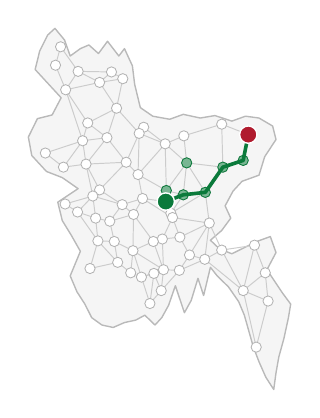
\begin{tikzpicture}[x=0.718cm, y=0.780cm]
    \fill[maplandfill] (0.320,5.820) -- (0.450,5.930) -- (0.620,5.740) -- (0.720,5.480) -- (0.900,5.600) -- (1.050,5.660) -- (1.220,5.520) -- (1.380,5.720) -- (1.580,5.480) -- (1.680,5.600) -- (1.820,5.320) -- (1.860,5.020) -- (1.960,4.640) -- (2.180,4.500) -- (2.480,4.450) -- (2.720,4.530) -- (3.020,4.470) -- (3.280,4.510) -- (3.580,4.420) -- (3.820,4.500) -- (4.060,4.470) -- (4.300,4.340) -- (4.360,4.120) -- (4.160,3.840) -- (4.060,3.540) -- (3.760,3.440) -- (3.600,3.280) -- (3.460,3.040) -- (3.560,2.840) -- (3.400,2.640) -- (3.200,2.480) -- (3.360,2.340) -- (3.580,2.260) -- (4.020,2.460) -- (4.260,2.540) -- (4.360,2.280) -- (4.200,2.000) -- (4.460,1.640) -- (4.620,1.440) -- (4.580,1.220) -- (4.500,0.880) -- (4.410,0.580) -- (4.360,0.320) -- (4.320,0.050) -- (4.180,0.250) -- (4.060,0.500) -- (3.960,0.740) -- (3.880,1.000) -- (3.800,1.260) -- (3.700,1.480) -- (3.520,1.720) -- (3.320,1.900) -- (3.200,2.040) -- (3.080,1.580) -- (2.980,1.860) -- (2.860,1.500) -- (2.740,1.300) -- (2.580,1.740) -- (2.460,1.420) -- (2.340,1.220) -- (2.220,1.100) -- (2.040,1.260) -- (1.880,1.180) -- (1.680,1.140) -- (1.480,1.060) -- (1.280,1.100) -- (1.100,1.220) -- (0.980,1.440) -- (0.840,1.640) -- (0.720,1.900) -- (0.900,2.300) -- (0.740,2.560) -- (0.580,2.800) -- (0.500,3.100) -- (0.860,3.320) -- (0.580,3.500) -- (0.300,3.600) -- (0.040,3.860) -- (-0.020,4.160) -- (0.140,4.460) -- (0.400,4.520) -- (0.560,4.800) -- (0.300,5.060) -- (0.100,5.260) -- (0.180,5.560) -- cycle;
    \draw[mapborder] (0.320,5.820) -- (0.450,5.930) -- (0.620,5.740) -- (0.720,5.480) -- (0.900,5.600) -- (1.050,5.660) -- (1.220,5.520) -- (1.380,5.720) -- (1.580,5.480) -- (1.680,5.600) -- (1.820,5.320) -- (1.860,5.020) -- (1.960,4.640) -- (2.180,4.500) -- (2.480,4.450) -- (2.720,4.530) -- (3.020,4.470) -- (3.280,4.510) -- (3.580,4.420) -- (3.820,4.500) -- (4.060,4.470) -- (4.300,4.340) -- (4.360,4.120) -- (4.160,3.840) -- (4.060,3.540) -- (3.760,3.440) -- (3.600,3.280) -- (3.460,3.040) -- (3.560,2.840) -- (3.400,2.640) -- (3.200,2.480) -- (3.360,2.340) -- (3.580,2.260) -- (4.020,2.460) -- (4.260,2.540) -- (4.360,2.280) -- (4.200,2.000) -- (4.460,1.640) -- (4.620,1.440) -- (4.580,1.220) -- (4.500,0.880) -- (4.410,0.580) -- (4.360,0.320) -- (4.320,0.050) -- (4.180,0.250) -- (4.060,0.500) -- (3.960,0.740) -- (3.880,1.000) -- (3.800,1.260) -- (3.700,1.480) -- (3.520,1.720) -- (3.320,1.900) -- (3.200,2.040) -- (3.080,1.580) -- (2.980,1.860) -- (2.860,1.500) -- (2.740,1.300) -- (2.580,1.740) -- (2.460,1.420) -- (2.340,1.220) -- (2.220,1.100) -- (2.040,1.260) -- (1.880,1.180) -- (1.680,1.140) -- (1.480,1.060) -- (1.280,1.100) -- (1.100,1.220) -- (0.980,1.440) -- (0.840,1.640) -- (0.720,1.900) -- (0.900,2.300) -- (0.740,2.560) -- (0.580,2.800) -- (0.500,3.100) -- (0.860,3.320) -- (0.580,3.500) -- (0.300,3.600) -- (0.040,3.860) -- (-0.020,4.160) -- (0.140,4.460) -- (0.400,4.520) -- (0.560,4.800) -- (0.300,5.060) -- (0.100,5.260) -- (0.180,5.560) -- cycle;
    \coordinate (panchagarh) at (0.550,5.630);
    \coordinate (thakurgaon) at (0.460,5.330);
    \coordinate (nilphamari) at (0.860,5.230);
    \coordinate (lalmonirhat) at (1.450,5.220);
    \coordinate (kurigram) at (1.650,5.110);
    \coordinate (rangpur) at (1.240,5.050);
    \coordinate (dinajpur) at (0.640,4.930);
    \coordinate (gaibandha) at (1.540,4.630);
    \coordinate (joypurhat) at (1.030,4.390);
    \coordinate (sunamganj) at (3.400,4.370);
    \coordinate (sherpur) at (2.020,4.320);
    \coordinate (jamalpur) at (1.940,4.220);
    \coordinate (sylhet) at (3.870,4.200);
    \coordinate (netrokona) at (2.730,4.180);
    \coordinate (bogura) at (1.370,4.150);
    \coordinate (naogaon) at (0.940,4.100);
    \coordinate (mymensingh) at (2.400,4.050);
    \coordinate (chapainawabganj) at (0.280,3.900);
    \coordinate (moulvibazar) at (3.780,3.780);
    \coordinate (sirajganj) at (1.710,3.750);
    \coordinate (kishoreganj) at (2.780,3.740);
    \coordinate (natore) at (1.000,3.720);
    \coordinate (rajshahi) at (0.600,3.670);
    \coordinate (habiganj) at (3.420,3.670);
    \coordinate (tangail) at (1.920,3.550);
    \coordinate (pabna) at (1.240,3.300);
    \coordinate (gazipur) at (2.420,3.290);
    \coordinate (brahmanbaria) at (3.110,3.260);
    \coordinate (narsingdi) at (2.720,3.220);
    \coordinate (kushtia) at (1.120,3.200);
    \coordinate (manikganj) at (2.000,3.160);
    \coordinate (dhaka) at (2.410,3.110);
    \coordinate (meherpur) at (0.630,3.070);
    \coordinate (rajbari) at (1.640,3.060);
    \coordinate (chuadanga) at (0.850,2.940);
    \coordinate (narayanganj) at (2.500,2.920);
    \coordinate (faridpur) at (1.840,2.900);
    \coordinate (munshiganj) at (2.530,2.850);
    \coordinate (jhenaidah) at (1.170,2.840);
    \coordinate (magura) at (1.420,2.790);
    \coordinate (cumilla) at (3.180,2.760);
    \coordinate (chandpur) at (2.660,2.530);
    \coordinate (shariatpur) at (2.350,2.500);
    \coordinate (jashore) at (1.210,2.470);
    \coordinate (narail) at (1.500,2.460);
    \coordinate (madaripur) at (2.190,2.460);
    \coordinate (khagrachhari) at (3.980,2.400);
    \coordinate (feni) at (3.400,2.320);
    \coordinate (gopalganj) at (1.830,2.310);
    \coordinate (lakshmipur) at (2.830,2.240);
    \coordinate (noakhali) at (3.100,2.170);
    \coordinate (khulna) at (1.560,2.120);
    \coordinate (satkhira) at (1.070,2.020);
    \coordinate (barishal) at (2.370,2.000);
    \coordinate (bhola) at (2.650,1.990);
    \coordinate (bagerhat) at (1.790,1.950);
    \coordinate (rangamati) at (4.170,1.950);
    \coordinate (jhalokati) at (2.200,1.940);
    \coordinate (pirojpur) at (1.980,1.880);
    \coordinate (patuakhali) at (2.330,1.660);
    \coordinate (chattogram) at (3.780,1.660);
    \coordinate (bandarban) at (4.220,1.490);
    \coordinate (barguna) at (2.130,1.450);
    \coordinate (coxsbazar) at (4.010,0.740);
    \foreach \a/\b in {panchagarh/thakurgaon, panchagarh/nilphamari, thakurgaon/dinajpur, nilphamari/dinajpur, nilphamari/rangpur, nilphamari/lalmonirhat, lalmonirhat/rangpur, lalmonirhat/kurigram, dinajpur/rangpur, dinajpur/joypurhat, dinajpur/naogaon, rangpur/kurigram, rangpur/gaibandha, kurigram/gaibandha, gaibandha/bogura, gaibandha/joypurhat, gaibandha/jamalpur, joypurhat/naogaon, joypurhat/bogura, naogaon/bogura, naogaon/natore, naogaon/chapainawabganj, naogaon/rajshahi, chapainawabganj/rajshahi, rajshahi/natore, natore/bogura, natore/sirajganj, natore/pabna, natore/kushtia, bogura/sirajganj, sirajganj/pabna, sirajganj/tangail, sirajganj/jamalpur, pabna/kushtia, pabna/rajbari, kushtia/chuadanga, kushtia/jhenaidah, kushtia/meherpur, kushtia/rajbari, meherpur/chuadanga, chuadanga/jhenaidah, chuadanga/jashore, jhenaidah/magura, jhenaidah/jashore, magura/narail, magura/faridpur, magura/rajbari, narail/jashore, narail/khulna, narail/gopalganj, jashore/satkhira, jashore/khulna, satkhira/khulna, khulna/bagerhat, bagerhat/pirojpur, bagerhat/gopalganj, gopalganj/faridpur, gopalganj/madaripur, gopalganj/pirojpur, gopalganj/barishal, rajbari/faridpur, rajbari/manikganj, faridpur/madaripur, faridpur/manikganj, madaripur/shariatpur, madaripur/barishal, shariatpur/chandpur, shariatpur/munshiganj, shariatpur/barishal, pirojpur/jhalokati, pirojpur/barguna, pirojpur/barishal, jhalokati/barishal, jhalokati/barguna, jhalokati/patuakhali, barguna/patuakhali, patuakhali/barishal, patuakhali/bhola, barishal/bhola, bhola/lakshmipur, bhola/noakhali, lakshmipur/noakhali, lakshmipur/chandpur, lakshmipur/cumilla, noakhali/cumilla, noakhali/feni, noakhali/chattogram, feni/cumilla, feni/chattogram, feni/khagrachhari, chandpur/cumilla, chandpur/munshiganj, cumilla/brahmanbaria, cumilla/munshiganj, brahmanbaria/narsingdi, brahmanbaria/kishoreganj, brahmanbaria/habiganj, brahmanbaria/narayanganj, narsingdi/kishoreganj, narsingdi/gazipur, narsingdi/narayanganj, narsingdi/dhaka, munshiganj/narayanganj, munshiganj/dhaka, munshiganj/manikganj, narayanganj/dhaka, dhaka/gazipur, dhaka/manikganj, gazipur/tangail, gazipur/mymensingh, gazipur/kishoreganj, manikganj/tangail, tangail/jamalpur, tangail/mymensingh, jamalpur/sherpur, jamalpur/mymensingh, sherpur/mymensingh, mymensingh/netrokona, mymensingh/kishoreganj, netrokona/kishoreganj, netrokona/sunamganj, kishoreganj/habiganj, habiganj/sunamganj, habiganj/moulvibazar, sunamganj/sylhet, sylhet/moulvibazar, khagrachhari/rangamati, khagrachhari/chattogram, rangamati/chattogram, rangamati/bandarban, bandarban/chattogram, bandarban/coxsbazar, chattogram/coxsbazar}
      {\draw[mapedge] (\a) -- (\b);}
    \foreach \n in {panchagarh, thakurgaon, nilphamari, lalmonirhat, kurigram, rangpur, dinajpur, gaibandha, joypurhat, sunamganj, sherpur, jamalpur, sylhet, netrokona, bogura, naogaon, mymensingh, chapainawabganj, moulvibazar, sirajganj, kishoreganj, natore, rajshahi, habiganj, tangail, pabna, gazipur, brahmanbaria, narsingdi, kushtia, manikganj, dhaka, meherpur, rajbari, chuadanga, narayanganj, faridpur, munshiganj, jhenaidah, magura, cumilla, chandpur, shariatpur, jashore, narail, madaripur, khagrachhari, feni, gopalganj, lakshmipur, noakhali, khulna, satkhira, barishal, bhola, bagerhat, rangamati, jhalokati, pirojpur, patuakhali, chattogram, bandarban, barguna, coxsbazar}
      {\node[mapdot] at (\n) {};}
    \foreach \n in {dhaka, narsingdi, gazipur, kishoreganj, brahmanbaria, habiganj, moulvibazar, sylhet}
      {\node[mapdot, fill=algastar!55, draw=algastar] at (\n) {};}
    \draw[maproute, draw=algastar] (dhaka) -- (narsingdi) -- (brahmanbaria) -- (habiganj) -- (moulvibazar) -- (sylhet);
  \node[mapstart] at (dhaka) {};
  \node[mapgoal] at (sylhet) {};
  \end{tikzpicture}
  \caption{A* search: 8 districts expanded, route 215.1\,km.}
  \label{fig:map-astar}
\end{subfigure}

  \caption{The districts expanded (filled) and the route returned by each
    algorithm from Dhaka (green) to Sylhet (red).}\label{fig:map-panels}
\end{figure}

Figure~\ref{fig:water} explains the gap. Flooding the map to $C^{*}$ submerges
the 50 districts with $g \le C^{*}$, which Dijkstra's algorithm expands, but only
the eight with $g + h \le C^{*}$, which A* expands
(Proposition~\ref{prop:expanded}).

\begin{figure}[htbp]
  \centering
  \begin{tabular}{@{}c@{\hspace{1em}}c@{}}
  {\footnotesize\textcolor{algdijkstra}{\textbf{Dijkstra}}: pin height $= g$} &
  {\footnotesize\textcolor{cbGreen}{\textbf{A*}}: pin height $= g + h$}\\[2pt]
  \waterpanel{0}{rbluemd} & \waterpanel{1}{cbGreen}\\
  {\footnotesize under water: \textbf{50} of 64} &
  {\footnotesize under water: \textbf{8} of 64 {\scriptsize\textcolor{neutralg}{(pins cut at 365\,km)}}}
\end{tabular}

  \caption{Every district as a pin, flooded to $C^{*} = 215.1$\,km. Left: pin
    height $g$. Right: pin height $g + h$. Adding $h$ lifts every district that
    lies away from Sylhet out of the water.}\label{fig:water}
\end{figure}

\subsection{Summary of the experiments}\label{sec:summary}

Table~\ref{tab:compare-all} collects all results. A* always returned a shortest
path, with 38\%, 41\% and 84\% fewer expansions than Dijkstra's algorithm on
the three instances. Greedy best-first search expanded the fewest vertices but
never returned a shortest path.

\begin{table}[htbp]
  \centering
  \caption{Vertices expanded and cost of the returned path on the three
    instances.}\label{tab:compare-all}
  \begin{tabular}{@{}lcccccc@{}}
    \toprule
     & \multicolumn{2}{c}{Running example} & \multicolumn{2}{c}{Grid}
     & \multicolumn{2}{c}{District graph}\\
    \cmidrule(lr){2-3}\cmidrule(lr){4-5}\cmidrule(l){6-7}
     & expanded & cost & expanded & cost & expanded & cost\\
    \midrule
    Dijkstra's algorithm     & 8 & 8 & 137 & 19 & 50 & 215.1\,km\\
    Greedy best-first search & 4 & \textcolor{cbRed}{10} & 48
      & \textcolor{cbRed}{35} & 6 & \textcolor{cbRed}{243.2\,km}\\
    A* search                & 5 & 8 & 81 & 19 & 8 & 215.1\,km\\
    \bottomrule
  \end{tabular}
\end{table}

\section{Variants of A*}\label{sec:variants}

Table~\ref{tab:variants} lists four variants of A* that address its
limitations: the dependence on the heuristic, the memory needed, and the cost of
searching from scratch after every change of the map.

\begin{table}[htbp]
  \centering
  \caption{Four variants of A* and the limitation that each one
    addresses.}\label{tab:variants}
  \small
  \renewcommand{\arraystretch}{1.25}%
  \begin{tabular}{@{}P{2.9cm}P{5.4cm}P{5.4cm}@{}}
    \toprule
    Variant & Idea & Limitation addressed\\
    \midrule
    Weighted A*~\cite{pohl1970}
      & rank by $g(v) + \varepsilon\, h(v)$ with $\varepsilon > 1$
      & too many expansions; with an admissible $h$, the returned path costs
        at most $\varepsilon C^{*}$\\
    IDA*~\cite{korf1985}
      & a series of searches that each follow one path at a time as far as
        possible (depth-first search), with a growing limit on $f$
      & memory: only the current path is stored, at the price of repeated
        expansions\\
    Jump point search~\cite{harabor2011}
      & skip the many paths of equal cost on uniform grids with diagonal moves
      & many equivalent expansions on grids; the path remains optimal\\
    D* Lite~\cite{koenig2002}
      & repair the previous search when the cost of an edge changes
      & maps that change while a robot or a game character moves\\
    \bottomrule
  \end{tabular}
\end{table}

\section{Conclusion}\label{sec:conclusion}

A* meets both requirements of Section~\ref{sec:requirements}. The cost so far
$g$ keeps it optimal, as in Dijkstra's algorithm, and the estimate $h$ directs
it toward the destination, as in greedy best-first search.

With a consistent heuristic, A* expands every vertex at most once and returns a
shortest path (Theorem~\ref{thm:consistent}). With an admissible but
inconsistent heuristic, a shortest path is guaranteed only when closed vertices
can be reopened (Theorem~\ref{thm:admissible}), and with an overestimating
heuristic no guarantee remains. The worst-case cost equals that of Dijkstra's
algorithm, but A* expands only vertices with $\delta(s,u) + h(u) \le C^{*}$
(Proposition~\ref{prop:expanded}). In our experiments it expanded 81 cells
against 137 on the grid and eight districts against 50 on the map of Bangladesh,
always returning a shortest path.

Since a larger admissible heuristic leaves fewer vertices to expand, choosing a
heuristic that is cheap and as close as possible to the true cost is the main
design decision when A* is applied to a new problem.

\paragraph{Code availability.} The programs that produce every trace, table and
experimental result of this report are available at \url{\repourl}.


\clearpage
\phantomsection
\addcontentsline{toc}{section}{References}
\bibliographystyle{unsrtnat}
\bibliography{references}
\end{document}
